% !TeX program = lualatex
\documentclass{article}
\usepackage{graphicx} % Required for inserting images
\usepackage{amsmath}
\usepackage{amsfonts}
\usepackage{amsthm}
\usepackage{amssymb}
\usepackage{float}
\usepackage{hyperref}
\usepackage{amssymb}
\usepackage{unicode-math}
\usepackage{colortbl}     % for \rowcolor
\usepackage{xcolor}       % for \definecolor
\usepackage{microtype}
\usepackage{booktabs}
\usepackage{array}
\usepackage{caption}

\definecolor{headerblue}{RGB}{30, 80, 140}
\definecolor{rowlight}{RGB}{235, 242, 252}
\definecolor{rowwhite}{RGB}{255, 255, 255}
\setmainfont{Latin Modern Roman}
\setmathfont{STIX Two Math} % <-- important

\title{Dissertação - João Paixão, Iago Leal}
\author{Bruno Llacer trotti}
\date{February 2026}

\theoremstyle{plain}   % <-- this keeps headings left-aligned
\newtheorem{theorem}{Theorem}
\newtheorem{lemma}{Lemma}
\newtheorem{remark}{Remark}
\newtheorem{conjecture}{Conjecture}
\newtheorem{corollary}{Corollary}
\newtheorem{proposition}{Proposition}
\newtheorem{definition}{Definition}
\newtheorem{example}{Example}
\newcommand{\extendR}{\overline{\mathbb{R}}}
\newcommand{\infcomp}{\overset{\rightharpoonup}{\circ}}
\newcommand{\supcomp}{\overset{\rightharpoondown}{\circ}}
\newcommand{\rtop}{\rotatebox{90}{$\top$}}
\newcommand{\mushroom}{⫏-}
\renewcommand{\arraystretch}{1.8}
\usepackage[
backend=biber,
style=alphabetic,
]{biblatex}

\addbibresource{bib.bib} %Imports bibliography file


\begin{document}

\maketitle
\tableofcontents
\section{Introduction}
Category theory has often been regarded as the mathematics of mathematics~\cite{maclane1998categories}.
The capacity to lift particular concepts into a more general and abstract space
has demonstrated, time and again, that not just the natural world,
but all of mathematics seems to be governed by universal constructions.
The investigation of such universal concepts allows us to see what a particular view
could not, and to realize the intrinsic connections and shared nature of what was once thought
to be separate.

One such field, that appears throughout mathematics
yet stands apart, is optimization.
Optimal thinking is present in every mathematical construct in which one seeks the
"ideal" object in some criterion. This notion of "ideal" often refers to the
simplest object that meets certain criteria. Prior work has already characterised the internal
optimization structure within categorical constructs \cite{Khadh2026bridging},
but such resuls still isolated; a unified treatment is still to be formalized.
Optimization should not serve as foundation for
other mathematical theories, but should itself be derived from them — in a way such that optimization
problems emerge from mathematical structure naturally.

This thesis is motivated by the observation that many important
mathematical structures used in optimization can be understood within
a single compositional framework \cite{stein2024compositional, hanks2024compositionalopt}.
Instead of treating relations, convex functions, quadratic forms, polyhedra,
and linear programs as isolated objects, this work shows that they can all be
interpreted as morphisms in categories whose composition is given by elimination or minimization.
In this way, optimization itself becomes an algebraic process and an emergent property of mathematics.


The development follows a natural progression.
Classical binary relations appear as Boolean-valued morphisms, weighted relations arise
through Lawvere quantales, convex bifunctions introduce infimal composition, quadratic
relations capture least-squares and energy minimization, polyhedral relations describe
systems of inequalities, and finally linear programming extends the framework to optimization
problems with decision variables and constraints. Each level enlarges the expressive power of
the previous one while preserving compositional structure.

This expressivity becomes especially apparent when analyzed through
the language of string diagrams \cite{joyal1991geometry, selinger2010survey, piedeleu2023introductionstringdiagramscomputer}.
Originating as a rigorous graphical language for
monoidal categories, string diagrams provide an intuitive yet mathematically
precise syntax in which the sequential and parallel composition of morphisms
correspond directly to vertical and horizontal juxtaposition of diagrams
\cite{joyal1991geometry, maclane1998categories}. Building on this foundation,
a rich family of \emph{diagrammatic} or \emph{graphical calculi} has emerged,
offering complete axiomatisations of various algebraic structures purely through
equational diagram rewriting \cite{selinger2010survey, bonchi2017interacting}.
These calculi have proved remarkably versatile, finding applications across a
wide range of fields: in \emph{quantum computing} \cite{coecke2011interacting};
\emph{electronics} \cite{baez2018compositional}; \emph{linear algebra} \cite{bonchi2017interacting,
bonchi2019affine, defreitas2025generalizinginvertiblematrixtheorem};
and in \emph{optimisation and probability} \cite{stein2024gqa,stein2025compositional,
bonchi2021polyhedral}.Throughout this work
we explore how, step by step, one can enrich the already known theories for linear
\cite{bonchi2017interacting} algebra by adding one new generator at a time, along with a particular
set of axioms, and derive even richer structures for convex problems \cite{stein2024compositional}.

We start by demonstrating how the addition of the new
generator of \textbf{GQA} \cite{stein2024gqa} expands the expressivity of previous theories
by acting as a sort of measurement device along the diagram. This new mechanic enables diagrams
to represent the broader class of weighted relations, rather than the more restricted class of binary relations.
From the optimization perspective, this is what plays the role of the objective function in a
optimization problem. More precisely, the language of \textbf{GQA} expresses minimization problems of
$\mathcal{l}_2$ norm of a vectors over some affine subspace, i.e. ,

\[
\inf_x \{\|Ax + b\|^2 : x \in S\}
\]

Next, we extend the Symmetric Monoidal Theory of \textbf{GAA} \cite{bonchi2019affine}
into the even more general theory of Symmetric Inequality Monoidal Theory.
This is achieved by adding the inequality generator $-\ge -$. Geometrically,
this allows our algebra to go beyond affine spaces and start representing polyhedral figures as linear inequality constraints in optimization.

\[
 \{| x \in P\} =
 \begin{cases}
     0 \quad if \;Ax +b\ge 0 \\
     +\infty \quad \text{otherwise}
 \end{cases}
\]

A key insight of this work is the interpretation of different classes of
relationswhithin an optimization-theoretic framework. By the theory of Lagragian Multipliers \cite{boyd2004convex}
, the constrains of optimization problems can be incorporated into the objective function via penalty
terms. This corresponce reveals that \textbf{indicator functions, i.e., binary relations,
play the role of constraints in the optimization setting}.

Figure~\ref{img:general_view} illustrates the path from the theory of interacting hopf algebras \cite{bonchi2017interacting}
to more expressive languages presented in this thesis, one generator at a time. It also illustrates how adding  a specific class
of "measurement" generators lifts the category from the binary relations category (indicator functions) into the one of
weighted relations (bifunctions/optimization problems).

\begin{figure}
    \centering
    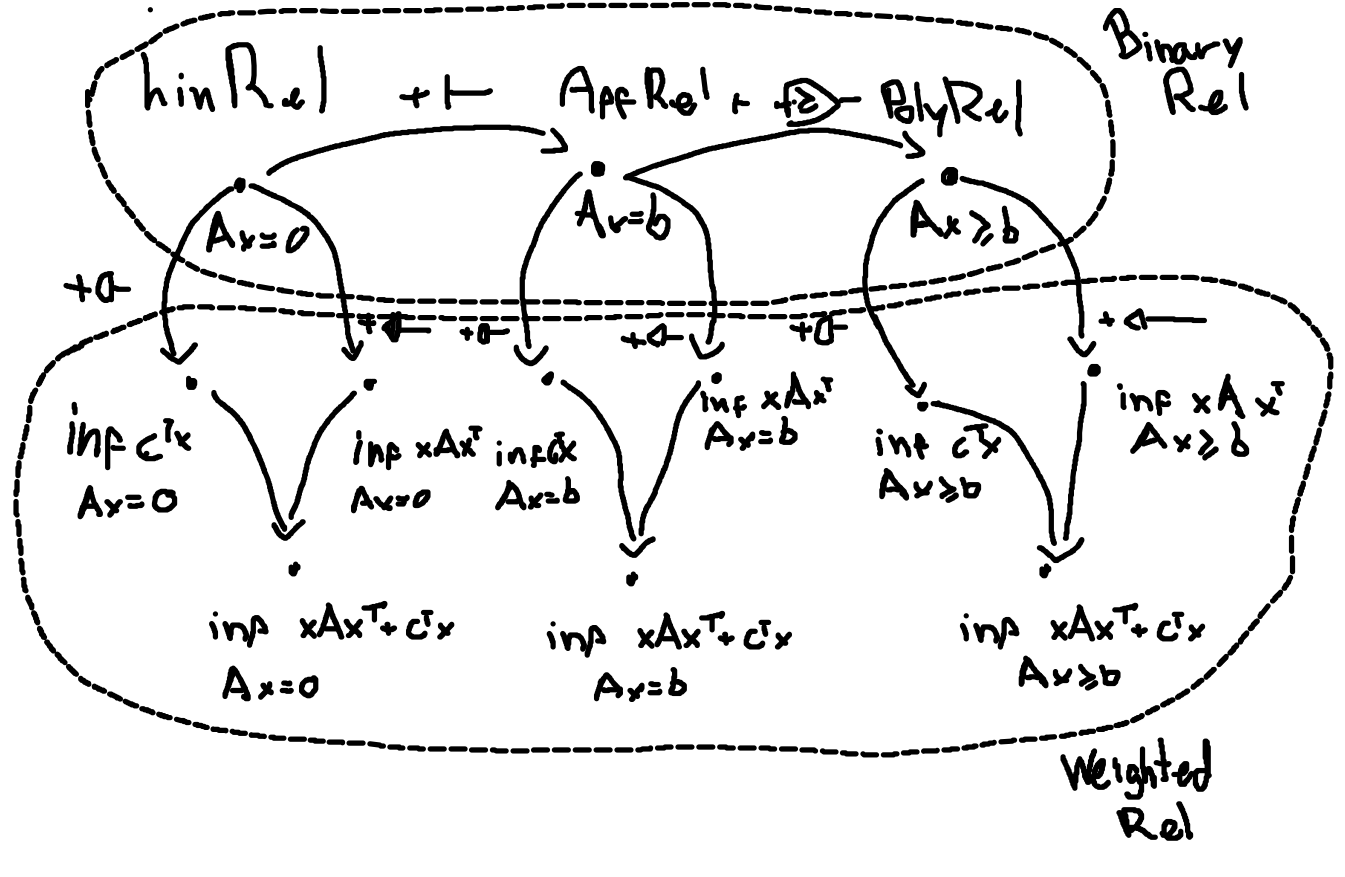
\includegraphics[width=1.0\linewidth]{images/Overview.png}
    \caption{This image represent the category of subcategories of Rel; We circle two class of subcategories,
    namely those that are contained in the Binary Relations categories and those embed in Weighted Relations category.
    Observe how morphism between objects (class of relations) are the addition of a single generator (along with some axioms),
    and that there are particular generators which are essential binary relations (those that are horizontal) that
    keeps objects in the subclass of binary relations, but there are others(the vertical morphisms),
    that resembles an output or measurement, that lift the relations to those on the Weighted Relations class
    }
    \label{img:general_view}
\end{figure}

Inspired by these observations, we make our central contribution
in the final section. The introduction of graphical
algebra for parametric linear programming. In this
setting, a linear program is no longer viewed only as
a numerical problem to be solved, but as a morphism that
can be composed with other optimization blocks.
This gives a symbolic language in which the elimination of internal variables corresponds directly to categorical composition, allowing optimization problems to be manipulated diagrammatically before computation.

This perspective is useful because it reveals that polyhedral convex functions and right-hand-side parametric linear programs are equivalent descriptions of the same mathematical object. In particular, every piecewise affine convex function can be represented as the value function of a linear program, which means the graphical LP theory provides a syntax for a broad class of nonsmooth convex models that appear in optimization, control, economics, and machine learning.

More broadly, the thesis suggests that graphical methods can play for optimization the same role that graphical linear algebra plays for matrices: providing normal forms, symbolic rewriting rules, and completeness results within a rigorous categorical setting. This opens the possibility of using diagrammatic reasoning not only for proofs, but also for designing compositional optimization systems and formal symbolic calculi for convex programming.

Thesis overview: In Section 2 we introduce the algebraic and categorical playground on which the rest
of the work is built, present the initial notions of quantales and relations, and how they play an interchangeable
role in a categorical view. Next, in Section 3, is introduced basic application of this theory to the
vast field of convex optimization \cite{stein2024compositional, Khadh2026bridging},
showing how many of its important constructs fall within such a categorical framework.
In Sections 4 and 5 is presented two already-known graphical theories, namely Graphical Quadratic
Algebra \cite{stein2024gqa} and Polyhedral Algebra \cite{bonchi2021polyhedral},
where some of the known proofs are recalled and refined.
Finally, we define and prove the completeness of an entirely new Graphical Algebra dedicated
to expressing parametric Linear Programs.

This work represents a first step toward a complete diagrammatic calculus for convex optimization.

\section{Ground definitions for relations}

In this section we explore the theory of relations.
While much of mathematical theory is built on functional thinking,
we argue that most of mathematics actually has a relational nature.
Category theory is the natural language for this purpose. It is precisely built on top of this notion,
in which everything one needs to know about an object is determined by its morphisms.

To begin we define the most basic kind of relation:

\begin{definition}[Binary Relations]
Let $X$ and $Y$ be sets. A \emph{binary relation} $R$ from $X$ to $Y$ is a subset
\[
R \subseteq X \times Y.
\]
Equivalently, it can be identified with its characteristic function
\[
\chi_R : X \times Y \to \{0,+\infty\},
\]
defined by
\[
\chi_R(x,y) =
\begin{cases}
0  \text{ if } (x,y) \in R,\\
+\infty \quad \text{otherwise}.
\end{cases}
\]
\end{definition}

A binary relation specifies wheather $x$ is related to $y$.
Observe that one can think of a relation in two different ways that will prove useful later.
First, as a set of pairs, where every relation is just a pair $(x,y) \in R$,
or as a map that has $x,y$ as inputs and outputs 0 if they are related, and $+\infty$ if they are not
the choice of $\infty$ is arbitrary and will be justified later. Normal choices here are actually $\{true,false\}$ or $\{0,1\}$)

This is a general construct as the sets $X$ and $Y$ can be anything.
We can, for instance, ask for further structures on such sets and obtain differents kinds of relations.
\begin{definition}[Linear/Affine Relations]
Let $X$ and $Y$ be vector spaces. A \emph{linear relation} from $X$ to $Y$ is a linear subspace
\[
R \subseteq X \times Y.
\]
An \emph{affine relation} is an affine subspace of $X \times Y$.

Equivalently, a linear relation can be described as the graph of a possibly multivalued linear operator, i.e.,
\[
R(x) := \{ y \in Y \mid (x,y) \in R \}.
\]

or, its characteristic function defined by
\[
\chi_R : X \times Y \to \{0,+\infty\},
\]

\[
\chi_R(x,y) =
\begin{cases}
0  \text{ if } (x,y) \in R,\\
+\infty \quad \text{otherwise}.
\end{cases}
\]

\end{definition}

Thus, a linear/affine relation is a binary relation where the set $R$ is a subspace

Notice, however, that we have been restricting the relations between $x$ and $y$ to be a case of "they are, or they are not related". In fact, we might be interested in adding degrees to such a relation, so that we could say that $x$ and $y$ are "more" or "less" related. This leads us to the well-known notion of weighted relations \cite{lawvere1973metric}.

\begin{definition}[Weighted Relations]
Let $X$ and $Y$ be any two sets and let $\extendR^+:= [0, +\infty]$.
A \emph{weighted relation} from $X$ to $Y$ is a set
\[
R \subseteq X \times Y \times \extendR^+
\]
such that for every $(x,y) \in X \times Y$ there exists \emph{exactly one}
$r \in \extendR^+$ satisfying
\[
(x,y,r) \in R.
\]

Equivalently, we may define the characteristic function
\[
\chi_R : X \times Y \to \extendR^+
\]
by
\[
\chi_R(x,y) =
r
\quad \text{if and only if } (x,y,r) \in R.
\]
\end{definition}

and the codomain is not restricted to a binary set anymore.
In fact, one could choose any other set instead of the $\extendR^+$ to be the codomain of the characteristic function as long as it satisfy some properties. In fact, the whole structure of a relation is further generalized by the notion of a quantale.
\begin{definition}[Quantale]
A \emph{quantale} is a structure $(Q,\leq,\otimes,e)$ such that:

\begin{itemize}
    \item $(Q,\leq)$ is a complete lattice, i.e., every subset $A \subseteq Q$ admits a join $\bigvee A$ and a meet $\bigwedge A$;
    \item $(Q,\otimes,e)$ is a monoid;
    \item Multiplication distributes over arbitrary join in each variable:
    \[
    a \otimes \Big( \bigvee_{i \in I} b_i \Big)
    =
    \bigvee_{i \in I} (a \otimes b_i),
    \qquad
    \Big( \bigvee_{i \in I} a_i \Big) \otimes b
    =
    \bigvee_{i \in I} (a_i \otimes b)
    \]
    for all families $\{a_i\}_{i\in I}, \{b_i\}_{i\in I} \subseteq Q$.
\end{itemize}

If $\otimes$ is commutative, the quantale is called \emph{commutative}.
If $e = \top$ (the top element of the lattice), it is called \emph{integral}.
\end{definition}

Given a quantale $Q$, we can define the notion of $Q$-valued relation \cite{coecke2018generalizedrelations}.

\begin{definition}[Generalized Relations]
A \emph{generalized relation} (or $Q$-valued relation) from $X$ to $Y$, where $Q$ is a quantale, is a set
\[
R \subseteq X \times Y \times Q
\]
such that for every $(x,y) \in X \times Y$ there exists \emph{exactly one}
$q \in Q$ satisfying
\[
(x,y,q) \in R.
\]

Its characteristic function is
\[
\chi_R: X \times Y \to Q
\]
defined by
\[
\chi_R(x,y) = q
\quad \text{if and only if } (x,y,q) \in R.
\]
\end{definition}

Now we are ready to build our previous relations as particular cases of this more general framework.

\begin{example}

The notion of a $Q$-valued relation recovers familiar concepts for particular choices of quantale.

\medskip

\noindent
\textbf{(1) Truth quantale.}
Let $Q = \{0,1\}$ with the usual order $0 \leq 1$, join given by $\lor$,
and monoidal product $\otimes = \land$ with unit $e = 1$.
This is the (Boolean) truth quantale.

A $Q$-valued relation is then a function
\[
R : X \times Y \to \{0,1\}.
\]
Such a function is precisely the characteristic function of an ordinary
binary relation
\[
\widetilde{R} \subseteq X \times Y,
\qquad
(x,y) \in \widetilde{R}
\;\Longleftrightarrow\;
R(x,y) = 1.
\]
Thus $Q$-valued relations coincide with classical binary relations.

\medskip

\noindent
\textbf{(2) Lawvere quantale.}
Let $Q = \extendR^+ = [0, +\infty]$ ordered by the
\emph{reverse} of the usual order (so that $a \leq b$ iff $a \geq b$
in the usual order), with monoidal product given by addition
\[
a \otimes b := a + b,
\]
and unit $e = 0$. Joins are then given by infima in the usual order.

This structure is the Lawvere quantale.
A $Q$-valued relation
\[
R : X \times Y \to \extendR^+
\]
is precisely a weighted relation assigning a (possibly infinite) cost
to each pair $(x,y)$.


\end{example}
Hence generalized relations unify ordinary binary relations and
weighted relations as special cases corresponding to particular quantales.

Note that linear and affine relations are not recovered by this construction,
since they demand extra structure
on the sets $X$ and $Y$, speciffically that $R$ be a linear or affine subspace of
$X \times Y$. They are, nonetheless,
fully embedded in the framework of binary relations.

Within this framework, we propose an extension of the Lawvere Quantale and
weighted relations called the Extended-Lawvere Quantale and
the Cost/Reward Relations, respectively. To our knowledge, this definition does
not appear elsewhere in the literature.

\begin{definition}[Optimization/Extended Lawvere Quantale]
Let
\[
\overline{\mathbb{R}} := \mathbb{R} \cup \{-\infty,+\infty\}.
\]
The \emph{optimization quantale} is the structure
\[
(\overline{\mathbb{R}},\geq,\otimes,e)
\]
defined as follows:

\begin{itemize}
    \item The order $\geq$ is the usual order on the extended real line.
    With this order, arbitrary joins are given by the usual infima:
    \[
    \bigvee A = \inf A.
    \]

    \item The monoidal product is addition:
    \[
    a \otimes b := a + b,
    \]
    where addition is extended in the usual way
    (with $a + (+\infty) = +\infty$ and
     $a + (-\infty) = -\infty$ whenever defined).

    \item The unit element is
    \[
    e := 0.
    \]
\end{itemize}

With these operations,
$(\overline{\mathbb{R}},\geq,+,0)$
is a commutative quantale. Joins are ordinary infima,
and addition distributes over arbitrary joins.
\end{definition}


\begin{definition}[Optimization (Cost/Reward) Relations]
Let $X$ and $Y$ be sets.
An \emph{optimization relation} from $X$ to $Y$ is an
$\overline{\mathbb{R}}$-valued relation, i.e., a function
\[
R : X \times Y \to \overline{\mathbb{R}}.
\]

Equivalently, it is a subset
\[
R \subseteq X \times Y \times \overline{\mathbb{R}}
\]
such that for every $(x,y) \in X \times Y$ there exists exactly one
$r \in \overline{\mathbb{R}}$ satisfying
\[
(x,y,r) \in R.
\]

The value $R(x,y)$ is interpreted as the objective value
(cost or reward) associated to the pair $(x,y)$,
with $+\infty$ and $-\infty$ representing extremal infeasibility
or unboundedness.
\end{definition}

Observe how this is essentially the weighted relations extended
along the negative values. The importance of it is that we want
to be able to express optimization problems that might be unfeasible
($+\infty$) or unbounded ($-\infty$), so we need to add both
the top and bottom element.

All of this admits a suitable and natural categorical construction.
Specifically, from any quantale $Q$ one can not only define $Q$-relations,
but also construct an entire category of them.
This category is the natural setting for discussing the
central concept of this framework: the composition of relations.

The following lemma shows how to build such a category and establishes
that this category also has a very important monoidal structure
behind it. Particularly, the category is a compact closed
symmetric monoidal category~\cite{maclane1998categories}:

\begin{proposition}[Category $\mathbf{Rel}(Q)$]
For a quantale $Q$, the $Q$-relations form a category \textbf{Rel}(Q) with composition and identities

\[
(S\circ R) (a,c) = \bigvee_b R(a,b) \otimes S(b,c) \quad 1_A(a,b) = \bigvee \{k | a=b\}
\]

If Q is a commutative quantale, then \textbf{Rel}(Q) carries a symmetric monoidal structure, with the categorical monoidal product $\bigotimes_{\mathcal{C}}$ on objects given by the Cartesian product of sets and the action on relations given for $R:A \to C$ and $S:B\to D$ by

\[
(R\otimes_{\mathcal{C}} S)(a,b,c,d) = R(a,c) \otimes S(b,d)
\]

The singleton set is the monoidal unit, and the category is compact closed w.r.t the monoidal structure
\end{proposition}

\begin{proof}
We verify the categorical structure.

\medskip
\noindent
\textbf{(1) Well-defined composition.}
Let $R:A \to B$ and $S:B \to C$ be $Q$-relations.
For each $(a,c) \in A \times C$, the set
\[
\{ R(a,b)\otimes S(b,c) \mid b \in B \}
\subseteq Q
\]
admits a supremum since $Q$ is a complete lattice.
Hence $(S\circ R)(a,c)$ is well-defined as an element of $Q$.

\medskip
\noindent
\textbf{(2) Associativity.}
Let $R:A\to B$, $S:B\to C$, and $T:C\to D$.
For $a\in A$, $d\in D$,
\[
((T\circ S)\circ R)(a,d)
=
\bigvee_{c}
\Big(
\bigvee_{b} R(a,b)\otimes S(b,c)
\Big)
\otimes T(c,d).
\]
Since $\otimes$ distributes over arbitrary suprema,
\[
=
\bigvee_{b,c}
R(a,b)\otimes S(b,c)\otimes T(c,d).
\]
Similarly,
\[
(T\circ (S\circ R))(a,d)
=
\bigvee_{b}
R(a,b)\otimes
\Big(
\bigvee_{c} S(b,c)\otimes T(c,d)
\Big)
=
\bigvee_{b,c}
R(a,b)\otimes S(b,c)\otimes T(c,d).
\]
Thus composition is associative.

\medskip
\noindent
\textbf{(3) Identities.}
For each set $A$, define
\[
1_A(a,b)
=
\begin{cases}
e & \text{if } a=b,\\
\bot & \text{otherwise},
\end{cases}
\]
where $\bot = \bigvee \varnothing$ is the bottom element of $Q$.

Then for $R:A\to B$,
\[
(R\circ 1_A)(a,b)
=
\bigvee_{a'}
1_A(a,a')\otimes R(a',b).
\]
All terms vanish except when $a'=a$, so
\[
=
e \otimes R(a,b)
=
R(a,b).
\]
Similarly, $1_B\circ R = R$. Hence identities exist.

\medskip
\noindent
\textbf{(4) Monoidal structure (commutative case).}
Assume $Q$ is commutative.
Define the tensor on objects by Cartesian product:
\[
A\otimes_{\mathcal{C}} B := A\times B.
\]
For relations $R:A\to C$ and $S:B\to D$, define
\[
(R\otimes_{\mathcal{C}} S)((a,b),(c,d))
=
R(a,c)\otimes S(b,d).
\]
Functoriality follows from associativity and commutativity of $\otimes$:
\[
(S_1\otimes S_2)\circ (R_1\otimes R_2)
=
(S_1\circ R_1)\otimes (S_2\circ R_2).
\]
The singleton set $1$ is a unit since $A\times 1 \cong A$.

Symmetry is induced by the swap map
\[
\sigma_{A,B}((a,b),(b',a'))=
\begin{cases}
e & \text{if } a=a',\, b=b',\\
\bot & \text{otherwise}.
\end{cases}
\]

\medskip
\noindent
\textbf{(5) Compact closure.}
For each set $A$, define unit and counit relations
\[
\eta : 1 \to A\times A,
\qquad
\epsilon : A\times A \to 1
\]
by
\[
\eta(*,(a,a')) =
\begin{cases}
e & a=a',\\
\bot & \text{otherwise},
\end{cases}
\qquad
\epsilon((a,a'),*) =
\begin{cases}
e & a=a',\\
\bot & \text{otherwise}.
\end{cases}
\]
A direct computation using the definition of composition shows that the
triangle identities hold:
\[
(1_A\otimes \epsilon)\circ (\eta\otimes 1_A) = 1_A,
\qquad
(\epsilon\otimes 1_A)\circ (1_A\otimes \eta) = 1_A.
\]
Thus every object is self-dual, and $\mathbf{Rel}(Q)$ is compact closed.
\end{proof}

A curious fact about relations is that they actually encode the notion of matrices and matrix multiplication. This serves as motivation for what will later become the diagrammatical theory of linear algebra. The following remark expands on it showing that every morphism in \textbf{Rel}$(Q)$ corresponds to a matrix with entries in $Q$, and that composition is exactly matrix multiplication.

\begin{remark}
A $Q$-valued relation $R : X \times Y \to Q$ is nothing but a
\emph{$Q$-valued matrix} indexed by $X \times Y$: one simply reads
off the entry at position $(x,y)$ as $\chi_R(x,y) \in Q$.
That is, a generalized relation is precisely an element of $Q^{X \times Y}$.

\medskip
\noindent
When $X$ and $Y$ are finite sets, say $|X| = m$ and $|Y| = n$,
this becomes completely explicit: a $Q$-valued relation is exactly
an $m \times n$ matrix
\[
  M_R \;=\; \bigl[\chi_R(x_i,\, y_j)\bigr]_{\substack{1 \leq i \leq m \\ 1 \leq j \leq n}}
  \;\in\; Q^{m \times n},
\]
whose $(i,j)$-entry records the $Q$-value assigned to the pair
$(x_i, y_j)$.

\medskip
\noindent
Moreover, composition of $Q$-valued relations corresponds precisely
to \emph{matrix multiplication in $Q$}.
Given a second $Q$-valued relation $S : Y \times Z \to Q$, their
composite $S \circ R : X \times Z \to Q$ is defined by
\[
  \chi_{S \circ R}(x, z)
  \;=\;
  \bigvee_{y \in Y}\, \chi_R(x,y) \otimes \chi_S(y,z),
\]
which, in matrix notation, reads
\[
  M_{S \circ R} \;=\; M_R \otimes M_S,
  \qquad
  (M_R \otimes M_S)_{ij}
  \;=\;
  \bigvee_{k=1}^{n}\, (M_R)_{ik} \otimes (M_S)_{kj}.
\]

This is exactly the usual row-times-column matrix product, but  with ordinary addition replaced by the join $\bigvee$ and ordinary  multiplication replaced by the monoidal product $\otimes$ of $Q$. The two axioms of a quantale — that $\otimes$ distributes over  arbitrary joins — are precisely what guarantees that this  multiplication is associative and well-defined, so that $Q$-valued  matrices form a category under this composition.
\end{remark}

To illustrate these new concepts, we look at some of our previous relations now built as categories.

\begin{example}[Category of Boolean relations]
Let
\[
Q = (\{0,1\}, \leq, \otimes, e)
\]
be the Boolean quantale where:
\begin{itemize}
    \item $0 \le 1$;
    \item $\otimes = \land$ (logical conjunction);
    \item $e = 1$;
    \item joins are given by $\lor$.
\end{itemize}

A $Q$-valued relation $R : A \to B$ is a function
\[
R : A \times B \to \{0,1\},
\]
which is precisely the characteristic function of a subset
\[
\widetilde{R} \subseteq A \times B.
\]

The composition formula in $\mathbf{Rel}(Q)$ becomes
\[
(S \circ R)(a,c)
=
\bigvee_{b} R(a,b) \land S(b,c).
\]
Since joins are logical disjunction, this reduces to
\[
(S \circ R)(a,c) = 1
\quad \Longleftrightarrow \quad
\exists b \in B \text{ such that }
R(a,b)=1 \text{ and } S(b,c)=1.
\]

Thus composition coincides exactly with the usual composition of binary relations.

Since the Boolean quantale is commutative,
$\mathbf{Rel}(Q)$ carries a symmetric monoidal structure:

\begin{itemize}
    \item On objects:
    \[
    A \otimes B := A \times B.
    \]

    \item On morphisms:
    \[
    (R \otimes S)((a,b),(c,d))
    =
    R(a,c) \land S(b,d).
    \]
\end{itemize}

The singleton set is the monoidal unit.
With this structure, $\mathbf{Rel}(Q)$ is precisely the classical
symmetric monoidal compact closed category $\mathbf{Rel}$.

\end{example}
\begin{example}[Category of weighted relations]\label{example:weighted-relations}
Let
\[
Q = (\mathbb{R}\cup\{+\infty\}, \le_Q, \otimes, e)
\]
be the Lawvere quantale where:
\begin{itemize}
    \item $a \le_Q b \iff a \ge b$ in the usual order;
    \item $\otimes = +$;
    \item $e = 0$;
    \item joins are given by infima in the usual order.
\end{itemize}

A $Q$-valued relation $R : A \to B$ is a function
\[
R : A \times B \to \mathbb{R} \cup \{+\infty\},
\]
assigning a cost (or weight) to each pair $(a,b)$.

The composition formula becomes
\[
(S \circ R)(a,c)
=
\inf_{b \in B}
\big(
R(a,b) + S(b,c)
\big).
\]

Thus composition is given by \emph{infimal convolution} (or shortest-path composition).

Since addition is commutative, the Lawvere quantale is commutative,
and $\mathbf{Rel}(Q)$ carries a symmetric monoidal structure:

\begin{itemize}
    \item On objects:
    \[
    A \otimes B := A \times B.
    \]

    \item On morphisms:
    \[
    (R \otimes S)((a,b),(c,d))
    =
    R(a,c) + S(b,d).
    \]
\end{itemize}

The singleton set is the monoidal unit.
With this tensor product, $\mathbf{Rel}(Q)$ is a symmetric monoidal
compact closed category of weighted relations.

In particular:
\begin{itemize}
    \item If $A,B,C$ are finite sets, relations may be viewed as matrices with entries in $\mathbb{R}\cup\{+\infty\}$.
    \item Composition is matrix multiplication in the $(\min,+)$-semiring.
\end{itemize}

Hence $\mathbf{Rel}(Q)$ is the category of weighted relations, which underlies dynamic programming, tropical algebra, and shortest-path problems.
\end{example}

Those examples illustrate how naturally the quantale structure supports  categorical constructions: composition of $Q$-valued relations corresponds  to matrix multiplication driven by $\otimes$, and the tensor product of  relations is governed by the join $\bigvee$, both operations coming  directly from the quantale axioms.

The resulting categories are symmetric monoidal, and it is precisely this monoidal backbone that will support the algebraic structure we aim to build. A key piece of that structure is a \emph{Frobenius monoid} on each object:  a monoid $(\mu, \eta)$ and a comonoid $(\delta, \varepsilon)$ on the same  object, satisfying the Frobenius law
\[
  (\mathrm{id} \otimes \mu) \circ (\delta \otimes \mathrm{id})
  \;=\;
  \delta \circ \mu
  \;=\;
  (\mu \otimes \mathrm{id}) \circ (\mathrm{id} \otimes \delta).
\]
A symmetric monoidal category in which every object carries such a  structure, compatibly with the tensor product, is called a  \emph{hypergraph category} \cite{fong2019hypergraph}.

Hypergraph categories are related to, but strictly more general than,
compact closed categories \cite{selinger2010survey}.
In a compact closed category every object $A$ has a dual $A^*$ with  unit $\eta_A : I \to A^* \otimes A$ and counit $\varepsilon_A : A \otimes A^* \to I$  satisfying the snake equations; a Frobenius structure does not require  the existence of such a dual. Conversely, if a compact closed category is such that every object is  self-dual ($A \cong A^*$) and the induced cups and caps satisfy the  Frobenius law, then it is a hypergraph category. Thus compact closed categories with self-dual
objects form a special  class of hypergraph categories, and it is the later, more general,  notion that we shall adopt as our ambient framework.
\begin{remark}
    If Q is commutative, then $\mathbf{Rel}(Q)$ is a hypergraph category and admits a commutative Frobenius structure on every object. Diagrammatically, we denote the additive and co-additive structure as

    \begin{figure}[H]
        \centering
        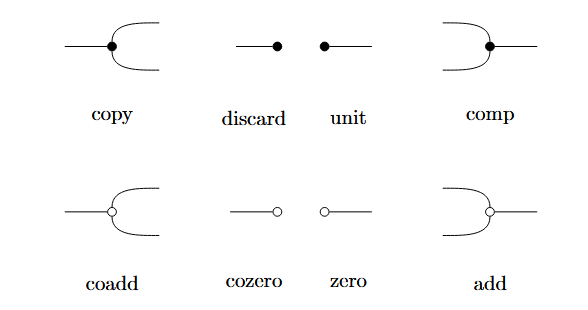
\includegraphics[width=1\linewidth]{images/froberniusDiagram.png}
        \caption{Frobernius additive(black) and co-additive(white) structure}
    \end{figure}

    Subject to the Frobernius Law (both colors)
   \begin{figure}[H]
        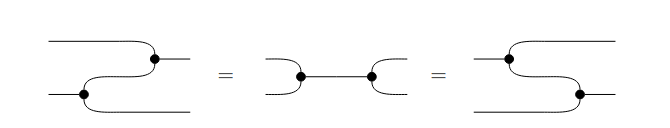
\includegraphics[width=1\linewidth]{images/FroberniusLaw.png}
    \end{figure}
\end{remark}

\begin{proof}
    Just a check that all laws do hold for any $\mathbf{Rel}(Q)$ category
\end{proof}

These constructions provide exactly the semantic foundation for the algebra we aim to build. In the same way that semantics is understood in linguistics and programming language theory \cite{winskel1993formal}, the semantics of a formal system assigns meaning to its expressions. More precisely, while syntax consists of the tokens and rules for forming and combining expressions, semantics is the interpretation assigned to each such expression — in our case, an optimization problem living in $\mathbf{Rel}(Q)$.

As outlined in the introduction, the central goal of this work is to show that optimization emerges naturally from algebraic and categorical structure.
The key mechanism enabling this is the infimal composition present in the definition of the Costs/Rewards category: composing two relations automatically performs variable elimination, which is precisely the fundamental operation underlying optimization.

To make this precise,
we need both a semantics — provided by the categorical framework developed above — and a syntax: a rigorous, compositional language for expressing optimization problems symbolically.
The map between those is structure-preserving map, a functor, from the syntactic layer into the semantic one.

The syntactic layer will be formalized as a Symmetric Monoidal Theory (SMT) \cite{bonchi2017interacting}, which is a presentation of a category by generators and equations, whose terms respect the compositional structure of a symmetric monoidal category. This is the standard tool for building graphical languages in the style of Graphical Linear Algebra, and it is the framework within which our completeness results will be stated and proved.

\begin{definition}[Symmetric Monoidal Theory]
    A SMT is a pair $(\Sigma,E)$, such that,  $\Sigma$ is a signature of operators $o$ that has arity $m$ and coarity $n$

    \medskip

$\Sigma$-terms are defined inductively as the smallest collection of
typed expressions $t : m \to n$ such that:

\begin{enumerate}

    \item (Generators) If $o \in \Sigma$ with $o : m \to n$, then $o$ is a $\Sigma$-term of type $m \to n$.
    \item (Identity)
    For every $n \in \mathbb{N}$, there is a term
    \[
        \mathrm{id}_n : n \to n.
    \]

    \item (Composition)
    If
    \[
        a : m \to n
        \quad \text{and} \quad
        b : n \to k
    \]
    are $\Sigma$-terms, then
    \[
        a ; b : m \to k
    \]
    is a $\Sigma$-term.

    \item (Tensor product)
    If
    \[
        a : m_1 \to n_1
        \quad \text{and} \quad
        b : m_2 \to n_2
    \]
    are $\Sigma$-terms, then
    \[
        a \otimes b : m_1 + m_2 \to n_1 + n_2
    \]
    is a $\Sigma$-term.

    \item (Symmetry)   For all $m,n \in \mathbb{N}$, there is a term
    \[
        \sigma_{m,n} : m+n \to n+m.
    \]
\end{enumerate}

\medskip

and $E$ be a set of equations over the $\Sigma-terms$.
\end{definition}

Often, we will think of elements $o:m\to n \in \Sigma$ as generators and represent them as string diagrams. Being the $\Sigma-terms$ the results of composing those generators horizontally and vertically inductively. The set $E$ as a collection of axiomatic equations over these string diagrams.

The categorical counterpart of these terms is the free category generated by the SMT.

\begin{definition}[The Free category of SMT]
    The $\text{FreeP}_{(\Sigma,E)}$ is the category freely generated by $(\Sigma,E)$ where the objects are natural numbers, morphisms are $\Sigma-terms$ quotiented by $E$, with composition and tensor product inherited from the symmetric monoidal structure. $\text{FreeP}_{(\Sigma,E)}$ is in fact a PROP\footnote{ For the definition of a prop see~\cite{maclane1998categories}}.
\end{definition}

The $\text{FreeP}_{(\Sigma,E)}$, also denoted as $P\Sigma_{/E}$,
\footnote{During the work we will use $\text{FreeP}_{S}$ and $S$, for
whatever syntax $S$ may be, interchangeably.}
will be our \textbf{syntax} responsible for expressing our underlying semantics.
For it to be considered a "useful" syntax we expect that it satisfies some properties, particularly we want it to be complete, sound and expressive.

Without those, our algebra would be empty since we would have no assurances that it actually says anything meaningful about we desire to say.

\begin{definition}
    We will say that a SMT axiomatizes or represents a specific category, usually called the semantic category, when the following diagram commutes:
    \begin{figure}[H]
        \centering
        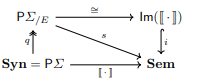
\includegraphics[width=0.35\linewidth]{images/Definibilty.png}
    \end{figure}
    where: $P\Sigma$ is the category where objects are natural numbers and morphisms are $\Sigma-terms$ from $n \to m$; $P\Sigma_{/E} = \text{FreeP}_{(\Sigma,E)}$ is the  $P\Sigma$ category with the morphisms quotiented by $E$ and there is then a prop morphism $q : P\Sigma \to P\Sigma_{/E}$ witnessing this quotient; $\textbf{Sem}$ is our semantic category (the Cost/Reward relations for example); and s is a full and faithful prop morphism. Another way to say the same is to demand two things out of the SMT, namely:
\begin{itemize}
    \item Soundness: We say that $P\Sigma_{/E}$ is sound if $c \overset{E}= d$\footnote{$\overset{E}=$ means that this equality is provable by the equations in $E$} implies $ [c] = [d]$.
    \item Completeness: We say that $P\Sigma_{/E}$ is complete if $[c] = [d]$ implies $c \overset{E}= d$
    \item Expressivity: We say that $P\Sigma_{/E}$ is expressive if for every morphism $c$ in \textbf{Sem} there exists $d \in P\Sigma_{/E}$ such that $[d] = c$
\end{itemize}


\end{definition}

Those three properties capture the idea that everything we can prove in the syntax, is a holds in the semantics (soundness), everything that holds in the semantics is provable in the syntax (completeness) and that every morphism in the semantics has a syntactic representative (expressivity). Moreover, these properties denote equivalent characteristics about the interpration map, both categorically and functionally. Below we depict a small table defining the equivalence between the desired properties and their equivalent statement:

\begin{table}[h!]
\centering
\caption{Equivalence of properties for the interpretation map
         $[\![{-}]\!] : P\Sigma_{/E} \to \mathbf{Sem}$}
\label{tab:equivalences}
\begin{tabular}{
  m{3.2cm}
  m{3.2cm}
  m{4.5cm}
}
\toprule
\textbf{Set theory} &
\textbf{Category theory} &
\textbf{Logic (SMT)} \\
\midrule

Total &
Functor &
Soundness: $c \overset{E}{=} d \;\Rightarrow\; [\![c]\!] = [\![d]\!]$ \\[6pt]

Deterministic &
Well-defined map &
(Functionality of the interpretation) \\[6pt]

Injective &
Faithful &
Completeness: $[\![c]\!] = [\![d]\!] \;\Rightarrow\; c \overset{E}{=} d$ \\[6pt]

Surjective &
Full &
Expressivity: $\forall\, f \in \mathbf{Sem},\; \exists\, d \in P\Sigma_{/E} \text{ s.t. } [\![d]\!] = f$ \\

\bottomrule
\end{tabular}
\end{table}

Now we introduce two of the foundational theories for Graphical Algebra, that will serve as a foundation for the following sections, namely, Graphical Linear Algebra~\cite{paixao2022highlevel, bonchi2017interacting} and Graphical Affine Algebra~\cite{bonchi2019affine}, we omit their definitions and proofs and refer to the original sources.

However, we do provide some notation on how to talk about those during the course of the work. Notice that, their semantics was already introduced when we talked about Linear/Affine relations.

\begin{definition}
    We will call $\textbf{GLA}$ the presentation of the Graphical Linear Algebra SMT, and, in the same manner, $\textbf{GAA}$ the SMT of Graphical Affine Algebra.
\end{definition}

\begin{definition}\label{def:arrows}
    We also denote with a $\overrightarrow{.}/\overleftarrow{.}$ when we want to talk about the algebra generated without the frobernius structure. For example $\overrightarrow{\textbf{GLA}}$ is the algebra generated by

    \begin{figure}[H]
        \centering
        
\includegraphics[width=.5\linewidth]{images/RightAlgebra.png}
    \end{figure}

    without their symmetric
    \begin{figure}[H]
        \centering
        
\includegraphics[width=0.5\linewidth]{images/LeftAlgebra.png}
    \end{figure}
    And the exactly opposite we denote as $\overleftarrow{\textbf{GLA}}$.
\end{definition}


%%%%%%%%%%%%%%%%%%%%%%%%%%%%%%%%%%%%%%%%%%%%%% TOWARDS CONVEX COMP %%%%%%%%%%%%%%%%%%%%%%%%%%$
\section{Composability of Convex Problems}

Having established the necessary categorical and algebraic tools,
we proceed to their application in convex analysis.
In this section we introduce a initial categorical framework for convex optimization
\cite{stein2024compositional}, showing how the fundamental operations of convex analysis —
infimal convolution, conjugation, and variable elimination —
arise naturally as categorical constructions. This gives the first concrete evidence that
optimization is not merely a collection of isolated techniques, but a coherent algebraic theory
with deep compositional structure.

The progression of the section is as follows.
We begin with the general category of bifunctions, which serves as the broadest setting,
and progressively restrict to convex bifunctions, where the analytical structure is richest.
We then introduce the Legendre--Fenchel transform and show that bifunction adjunction defines a contravariant functor between the convex and concave bifunction categories. These results lay the groundwork for the graphical theories developed in the following sections: Graphical Quadratic Algebra and Polyhedral Algebra will both arise as full subcategories of $\mathbf{CxBiFn}$, each corresponding to a class of bifunctions with additional algebraic structure.

Later, we will see the particular applications of such definitions and results.
For now, however, we begin by defining the broadest category in the hierarchy, which will
generalize most of the later work: the category of bifunctions.

\begin{definition}[Bifunction Category]
The category $\mathbf{BiFunc}$ is defined as follows:

\begin{itemize}
    \item Objects are sets.

    \item A morphism $F : A \to B$ is a function
    \[
    F : A \times B \to \overline{\mathbb{R}}.
    \]

    \item Given $F : A \to B$ and $G : B \to C$, their composition
    $G \circ F : A \to C$ is defined pointwise by
    \[
    (G \circ F)(a,c)
    :=
    \inf_{b \in B}
    \big(
        F(a,b) + G(b,c)
    \big).
    \]

    \item The identity morphism on an object $A$ is the function
    \[
    1_A : A \times A \to \overline{\mathbb{R}}
    \]
    given by
    \[
    1_A(a,a')
    =
    \begin{cases}
    0 & \text{if } a=a',\\
    +\infty & \text{otherwise}.
    \end{cases}
    \]
\end{itemize}

\medskip

If we equip $\mathbf{BiFunc}$ with a monoidal structure:

\begin{itemize}
    \item The tensor product on objects is the Cartesian product
    \[
    A \otimes B := A \times B.
    \]

    \item For morphisms $F : A \to C$ and $G : B \to D$,
    their tensor product
    \[
    F \otimes G : A \times B \to C \times D
    \]
    is defined by
    \[
    (F \otimes G)((a,b),(c,d))
    :=
    F(a,c) + G(b,d).
    \]
\end{itemize}

The singleton set serves as the monoidal unit.
\end{definition}

\begin{remark}
The category $\mathbf{BiFunc}$ is isomorphic to the category $\textbf{Rel}Q$ for
a suitable choice of $Q$.

Consider the quantale
\[
Q = (\overline{\mathbb{R}},\le_Q,\otimes,e)
\]
where:
\begin{itemize}
    \item $\overline{\mathbb{R}} = \mathbb{R} \cup \{-\infty,+\infty\}$;
    \item the order is reversed with respect to the usual order,
    \[
    a \le_Q b \quad \Longleftrightarrow \quad a \ge b
    \quad \text{(usual order)};
    \]
    \item the monoidal product is addition,
    \[
    a \otimes b := a + b;
    \]
    \item the unit is $e = 0$.
\end{itemize}

In this quantale, arbitrary joins are given by infima in the usual order:
\[
\bigvee\nolimits_Q A = \inf A.
\]

Now a $Q$-valued relation $R : A \to B$ is precisely a function
\[
R : A \times B \to \overline{\mathbb{R}},
\]
i.e.\ a bifunction. Moreover, the composition formula in
$\mathbf{Rel}(Q)$ becomes
\[
(S \circ R)(a,c)
=
\bigvee_{b} R(a,b)\otimes S(b,c)
=
\inf_{b}
\big(
R(a,b) + S(b,c)
\big),
\]
which is exactly the composition law in $\mathbf{BiFunc}$.

Therefore, $\mathbf{BiFunc}$ is (strictly) the same category as
$\mathbf{Rel}(Q)$ for the Lawvere-type quantale
$(\overline{\mathbb{R}}, \ge, +, 0)$.
\end{remark}

Bifunctions are fundamental objects in convex analysis \cite{rockafellar1970convex}.
They provide a unified language for expressing objective functions, feasibility constraints,
and duality simultaneously. The following proposition confirms that the framework is conservative:
classical set-theoretic relations embed faithfully into this richer setting.


\begin{proposition}
   The category of Binary Relations, i.e. the Boolean-relation is embed as a full subcategory of BiFunc.
\end{proposition}

\begin{proof}
    Just consider the functor $F:\mathbf{Rel}(B) \to \mathbf{BiFunc}$ that takes every morphism $R: X\to Y$, which is a subset of $X \times Y$, and maps it into the characteristic function $\chi_R: X\times Y \to \{0, +\infty\}$, also known as the indicator function $1_R(x,y)$, or in bracket notation $\{| (x,y) \in R|\} $
\end{proof}

Having established the general framework, we now restrict our attention to the convex setting, which is the natural home for optimization. The key insight is that convexity is preserved under infimal composition, so the convex bifunctions form a subcategory of $\mathbf{BiFunc}$ that is closed under the categorical operations.

\begin{definition}[Convex Bifunction Category $\mathbf{CxBiFn}$]
Let
\[
Q := (\overline{\mathbb{R}}, \le_Q, \otimes, e)
\]
be the extended-Lawvere quantale where:
\begin{itemize}
    \item $\overline{\mathbb{R}} = \mathbb{R} \cup \{-\infty,+\infty\}$;
    \item $a \le_Q b \iff a \ge b$ in the usual order;
    \item $a \otimes b := a + b$;
    \item $e := 0$.
\end{itemize}

The category $\mathbf{CxBiFn}$ is defined as follows:

\begin{itemize}
    \item \textbf{Objects:} finite-dimensional real vector spaces.

    \item \textbf{Morphisms:}
    A morphism $F : A \to B$ is a function
    \[
    F : A \times B \to \overline{\mathbb{R}}
    \]
    satisfying:
    \begin{itemize}
        \item $F$ is proper (not identically $+\infty$);
        \item $F$ is convex as a function on the product space $A \times B$;
        \item $F$ is lower semicontinuous.
    \end{itemize}

    \item \textbf{Composition:}
    Given $F : A \to B$ and $G : B \to C$, their composite
    \[
    G \circ F : A \to C
    \]
    is defined by infimal convolution:
    \[
    (G \circ F)(a,c)
    :=
    \inf_{b \in B}
    \big(
        F(a,b) + G(b,c)
    \big).
    \]

    \item \textbf{Identity:}
    For each object $A$, the identity morphism
    \[
    1_A : A \to A
    \]
    is given by
    \[
    1_A(a,a')
    =
    \begin{cases}
    0 & \text{if } a=a',\\
    +\infty & \text{otherwise}.
    \end{cases}
    \]

    \item Monoidal product
    \begin{itemize}
    \item On objects:
    \[
    A \otimes B := A \times B.
    \]

    \item On morphisms:
    For $F : A \to C$ and $G : B \to D$,
    \[
    (F \otimes G)((a,b),(c,d))
    :=
    F(a,c) + G(b,d).
    \]

    \item The monoidal unit is the zero-dimensional vector space $\{0\}$.
\end{itemize}
\end{itemize}
\end{definition}

\begin{remark}
    One may define the analogous category $\mathbf{CvBiFn}$ which is the category of concave bi functions. For doing so, one should only change the composition from inf to sup, this is:

    \[
    (G \circ F)(a,c)
    :=
    \sup_{b \in B}
    \big(
        F(a,b) + G(b,c)
    \big).
    \]

    Every result for $\mathbf{CxBiFn}$ will hold, in a equivalent way, to the category $\mathbf{CvBiFn}$
\end{remark}

\begin{remark}
Every finite-dimensional real vector space $V$ is linearly isomorphic to
$\mathbb{R}^n$, where $n = \dim V$.

Hence, one may restrict the objects of $\mathbf{CxBiFn}$ to the family
\[
\mathrm{Ob}(\mathbf{CxBiFn})
=
\{ \mathbb{R}^n \mid n \in \mathbb{N} \}.
\]
With this choice, $\mathbf{CxBiFn}$ becomes a skeletal category,
since $\mathbb{R}^n \cong \mathbb{R}^m$ implies $n=m$.

Also, if one considers the isomorphism $n \leftrightarrow \mathbb{R}^n$, $\mathbf{CxBiFn}$ becomes a prop, this can be made strict by defining the monoidal product on objects as sum.

\[
m\otimes n = m+n
\]

which is isomorphic to

\[
\mathbb{R}^m \otimes \mathbb{R}^m  = \mathbb{R}^m \times \mathbb{R}^m = \mathbb{R}^{m+n}
\]
\end{remark}

Observe that we have constructed a category whose morphisms
are interpreted as convex optimization problems.
Since every bifunction $F: \mathbb{R}^m \times \mathbb{R}^n
\to \extendR$ can be written as

\[
F(x,y) = \inf_{z} z \quad s.t \;z=F(x,y)
\]

This observation is central to the thesis. It shows that there's some sort of duality between relations and optimization.
For a single morphism, however, this remains imprecise.
The compositional structure yields more substantive insights.

\[
(S\circ R)(x,z)=\inf_y \{R(x,y)+S(y,z)\}
\]
Which shows that relational composition is precisely variable elimination: composing two relations automatically marginalises over the intermediate variable $y$ by minimising the combined cost. In the binary case this reduces to the existential question of whether a mediating element exists; in the weighted case it asks for the *optimal* such element. Optimization is therefore not imposed on the categorical structure from outside — it emerges from composition itself.

Convex theory also has a very nice duality theory which is of particular interest in algebraic constructs such as this one. We now introduce the central duality operation of convex analysis The Legendre--Fenchel transform.

\begin{definition}[Legendre-Fenchel Transform]
    For a convex function $f:\mathbb{R}^n \to \overline{\mathbb{R}}$, its convex
    conjugate $f^*:\mathbb{R}^n \to \overline{\mathbb{R}}$ is defined as:
    \[
        f^*(x^*) = \sup_x \left\{ \langle x^*, x \rangle - f(x) \right\}.
    \]
\end{definition}

Geometrically, $f^*$ encodes information about all affine functions majorised
by $f$: each supporting hyperplane of the epigraph of $f$ corresponds to a
point where $f^*$ is finite \cite{rockafellar1970convex}. This duality plays a
central role across many fields in mathematics and physics such as convex
optimization and duality \cite{boyd2004convex},
probability theory and large deviations~\cite{dembo2010large},
optimal transport~\cite{villani2009optimal} and Hamiltonian mechanics.

The Legendre--Fenchel transform plays a role in convex optimization analogous to that of transposition in linear algebra: it exchanges the roles of primal and dual variables, and, as we shall see, it interacts functorially with categorical composition \cite{willerton2015legendre}.

Such transformation can be extended to bifunctions providing the equivalent of the Legendre--Fenchel transform for morphisms in \textbf{CvBiFn}, providing a notion of duality that is compatible with categorical composition.

\begin{definition}[Adjoint of convex bifunctions]
    The adjoint of a convex bifunction $F$ is the concave bifunction $F^*$ defined by
    \[
    F^*(y^*,x^*) = \inf_{x,y} \{ F(x,y) + \langle x^*,x\rangle - \langle y^*,y\rangle \}
    \]

    Note that $F^*$ is a closed concave bifunction and $F^{**} = \text{cl}(F)$, also, if $F$ is closed, then:
    \[
    F^{**} = F
    \]
\end{definition}

The following theorem is the central result of this section. It shows that bifunction adjunction is not merely an analytic operation, but a categorical one: it defines a contravariant functor between $\mathbf{CxBiFn}$ and $\mathbf{CvBiFn}$. This is the bifunction analogue of the fact that matrix transposition reverses composition, and it will be the algebraic basis for the duality diagrams appearing in the graphical theories of the next sections.


\begin{theorem}[Functoriality of the bifunction adjoint]
Let $F:\mathbb{R}^m \times \mathbb{R}^n \to \overline{\mathbb{R}}$
and
$G:\mathbb{R}^n \times \mathbb{R}^p \to \overline{\mathbb{R}}$
be proper, convex, and lower semicontinuous functions.

Define their infimal composition
\[
(G \infcomp F)(x,z)
:=
\inf_{y \in \mathbb{R}^n}
\big\{
F(x,y) + G(y,z)
\big\}.
\]

Assume that a standard qualification condition holds, e.g.
\[
\operatorname{ri}(\operatorname{dom} F)
\cap
\operatorname{ri}(\operatorname{dom} G)
\neq \varnothing
\]
in the $y$-variable.

Then
\[
(G \infcomp F)^*
=
F^* \supcomp G^*,
\]
where the supremal composition is defined by
\[
(F^* \supcomp G^*)(z^*,x^*)
:=
\sup_{y^* \in \mathbb{R}^n}
\big\{
F^*(y^*,x^*)
+
G^*(z^*,y^*)
\big\}.
\]

 Hence it defines a contravariant functor between the category $\mathbf{CxBiFn}$ and the category $\mathbf{CvBiFn}$.
\end{theorem}

\begin{proof}
Let $F:\mathbb{R}^m \times \mathbb{R}^n \to \overline{\mathbb{R}}$
and
$G:\mathbb{R}^n \times \mathbb{R}^p \to \overline{\mathbb{R}}$
be proper, convex, and lower semicontinuous.
Define
\[
H(x,z) := (G \infcomp F)(x,z)
=
\inf_{y \in \mathbb{R}^n}
\{ F(x,y) + G(y,z) \}.
\]

\medskip


By definition,
\[
H^*(z^*,x^*)
=
\inf_{x,z}
\left\{
H(x,z)
+ \langle x^*,x\rangle
- \langle z^*,z\rangle
\right\}.
\]
Substituting the definition of $H$,
\[
H^*(z^*,x^*)
=
\inf_{x,z}
\inf_{y}
\Big\{
F(x,y) + G(y,z)
+ \langle x^*,x\rangle
- \langle z^*,z\rangle
\Big\}.
\]
Since the infimum is taken over independent variables,
\[
H^*(z^*,x^*)
=
\inf_{x,y,z}
\Big\{
F(x,y) + G(y,z)
+ \langle x^*,x\rangle
- \langle z^*,z\rangle
\Big\}.
\]

\medskip


Insert the identity
\[
0
=
\sup_{y^*}
\{
\langle y^*,y\rangle
-
\langle y^*,y\rangle
\}
\]
to prepare for dualization:
\[
H^*(z^*,x^*)
=
\inf_{x,y,z}
\sup_{y^*}
\Big\{
F(x,y) + \langle x^*,x\rangle
- \langle y^*,y\rangle
+
G(y,z)
+ \langle y^*,y\rangle
- \langle z^*,z\rangle
\Big\}.
\]

\medskip


Under the qualification condition
\[
\operatorname{ri}(\operatorname{dom}F)
\cap
\operatorname{ri}(\operatorname{dom}G)
\neq \varnothing
\quad \text{in the $y$-variable},
\]
Fenchel–Rockafellar duality (or a standard minimax theorem)
allows the interchange of $\inf$ and $\sup$:
\[
H^*(z^*,x^*)
=
\sup_{y^*}
\inf_{x,y,z}
\Big\{
F(x,y) + \langle x^*,x\rangle
- \langle y^*,y\rangle
+
G(y,z)
+ \langle y^*,y\rangle
- \langle z^*,z\rangle
\Big\}.
\]

\medskip


The expression separates into two independent infima:
\[
=
\sup_{y^*}
\left\{
\inf_{x,y}
\big(
F(x,y)
+ \langle x^*,x\rangle
- \langle y^*,y\rangle
\big)
+
\inf_{y,z}
\big(
G(y,z)
+ \langle y^*,y\rangle
- \langle z^*,z\rangle
\big)
\right\}.
\]

\medskip

By definition of the bifunction adjoint,
\[
F^*(y^*,x^*)
=
\inf_{x,y}
\big\{
F(x,y)
+ \langle x^*,x\rangle
- \langle y^*,y\rangle
\big\},
\]
and
\[
G^*(z^*,y^*)
=
\inf_{y,z}
\big\{
G(y,z)
+ \langle y^*,y\rangle
- \langle z^*,z\rangle
\big\}.
\]
Hence
\[
H^*(z^*,x^*)
=
\sup_{y^*}
\big\{
F^*(y^*,x^*)
+
G^*(z^*,y^*)
\big\}.
\]

\medskip

Therefore,
\[
(G \infcomp F)^*
=
F^* \supcomp G^*,
\]
where
\[
(F^* \supcomp G^*)(z^*,x^*)
=
\sup_{y^*}
\{ F^*(y^*,x^*) + G^*(z^*,y^*) \}.
\]

Finally, since the Fenchel conjugation is involutive on proper,
convex, lower semicontinuous functions, we also have $H^{**} = H$,
and the adjoint reverses composition. This completes the proof.
\end{proof}

The results of this section establish $\mathbf{CxBiFn}$ as a well-behaved categorical setting for convex optimization. The two special classes of morphisms — quadratic bifunctions and polyhedral bifunctions — each inherit this structure while admitting a finite, explicit representation. It is precisely this finiteness that makes a graphical algebra possible: in both cases, morphisms can be encoded as diagrams composed from a finite set of generators, and the equational theory of the diagrams corresponds exactly to the equivalences between optimization problems.
The following two sections make this precise.


%%%%%%%%%%%%%%%%%%%%%%%%%%%%%%%%% QUADRATIC RELATIONS %%%%%%%%%%%%%%%%%%%%%%%%%%%%%%%%%%%%%

\section{Quadratic Relations}

Among all convex bifunctions, quadratic ones are particularly well-structured:
they are the simplest class rich enough to express least-squares problems, energy minimisation, and Gaussian inference, yet structured enough to admit a finite diagrammatic presentation. This section develops the Graphical Quadratic Algebra (GQA) \cite{stein2024gqa}, the first of the two graphical theories on which our linear programming algebra will be built.
We begin with the necessary preliminaries on quadratic functions, then define the symmetric monoidal theory whose morphisms are non-negative quadratic optimization problems — the non-negativity condition ensuring that infimal composition is always well-posed. We then present the soundness and completeness results for this theory. The section closes by deriving several known results about quadratic problems purely through string diagram manipulation, demonstrating that the graphical syntax is not merely a notational convenience but a genuine calculus in which optimization arguments can be carried out.
\subsection{Preliminary results about quadratic functions}

Our main interest are non-negative quadratic functions. The motivation for this
unusual choice is that we want to avoid unbounded problems remain on convex settings, since negative quadratic functions
may be concave. Formally,
this means that the category of partial non-negative quadratic functions embeds into the positive
Lawvere-quantale.

Next, we rigorously define the notion of a non-negative quadratic function
along with other relevant equivalence results.

\begin{definition}
    A partial quadratic function is a function
\[
f : \mathbb{R}^{n+m} \to [0,+\infty]
\]
of the form
\[
f(x,y) = \langle x, Ax\rangle + \langle b, x\rangle + c +\{| x \in M|\}
\]
where $A$ is a symmetric matrix, $M$ is an affine subspace, $b \in \mathbb{R}^n$ and $c \in \mathbb{R}$ and $\langle-,-\rangle$ denotes the usual inner product on the reals.
\end{definition}

\begin{definition}
    An elementary convex partial quadratic function $h$ is a function that can be written in the diagonal form $h(x) = \sum_i \lambda_i x_i^2$ for $\lambda_i \ge 0$. It is partial because $h(x) = \infty$ whener $\lambda_i = +\infty$ $x_i \neq 0$ for some $i$.
\end{definition}

\begin{proposition}\label{prop:PQFEquivalence}
    The following statements are equivalent
    \begin{itemize}
        \item $f$ is a non-negative partial quadratic function
        \item $f$ can be written in the form $f(x) = h(A(x-a)) + c$ where $A$ is an invertible matrix, $c \ge 0$ and $h$ an elementary convex partial quadratic function
        \item $f$ can be written as $f(x) = \inf \{ ||y||^2: (x,y) \in M\}$ where $M$ is an affine subspace
    \end{itemize}
\end{proposition}


\begin{proof}[Proof of Proposition 2]

\noindent
\textbf{(1) $\Rightarrow$ (2).}
Using an affine change of coordinates, we may assume that the domain of $f$
is the subspace
\[
M=\mathbb{R}^m \times \{0\}.
\]
Define the restricted function
\[
\tilde f(x_1,\dots,x_m)
=
f(x_1,\dots,x_m,0,\dots,0).
\]
Then $\tilde f$ is a total nonnegative quadratic function. Hence, by the
characterisation of total nonnegative quadratic functions,
there exist an invertible matrix $A$, a vector $a$, a constant $c\ge 0$,
and an elementary convex quadratic function $h$ such that
\[
\tilde f(x_1,\dots,x_m)
=
h\big(A((x_1,\dots,x_m)-a)\big)+c.
\]
Returning to the original coordinates, we obtain
\[
f(x)
=
h\big(A((x_1,\dots,x_m)-a)\big)
+ \infty \cdot x_{m+1}
+ \cdots
+ \infty \cdot x_n
+ c,
\]
which is of the required form.

\medskip
\noindent
\textbf{(2) $\Rightarrow$ (3).}
Under the affine coordinate change
\[
y = A(x-a),
\]
it suffices to consider functions of the form
\[
f(y)=h(y)+c,
\]
where $h$ is an elementary quadratic function. Up to a permutation of
coordinates, we may write
\[
h(y_1,y_2,y_3)
=
\|y_1\|_2^2
+
\{\, y_3=0 \,\},
\]
where $\{\, y_3=0 \,\}$ denotes the indicator function of the subspace
$\{y_3=0\}$ (equal to $0$ if $y_3=0$ and $+\infty$ otherwise).

Define the affine relation
\[
M
=
\left\{
\big((y_1,y_2,y_3),(y_1,\sqrt{c})\big)
\;\middle|\;
y_3=0
\right\}.
\]
Then, for every $x$,
\[
f(x)
=
\inf\{\|z\|_2 : (x,z)\in M\}.
\]

\medskip
\noindent
\textbf{(3) $\Rightarrow$ (1).}
Let $M\subset \mathbb{R}^n\times\mathbb{R}^m$ be an affine relation.
Then there exists a vector subspace $D\subset \mathbb{R}^m$ and an affine map
$g:\mathbb{R}^n\to D^\perp$ such that, for each $x$,
\[
M_x
=
\{y : (x,y)\in M\}
=
\begin{cases}
g(x)+D, & x\in \pi_X M,\\
\varnothing, & \text{otherwise},
\end{cases}
\]
where $\pi_X M$ denotes the projection of $M$ onto $\mathbb{R}^n$.

Hence,
\[
\inf\{\|y\|_2 : y\in M_x\}
=
\|g(x)\|_2
+
\{\, x\in \pi_X M \,\}.
\]
This is clearly a nonnegative partial quadratic function.
\end{proof}

As it is stated above, a non-negative partial quadratic function has a very convenient algebraic
structure that can be expressed both with and without explicit constrains.

This formulation reveals one of the deepest conceptual payoffs of the relational framework.  In the standard convex analysis view \cite{boyd2004convex}, incorporating a constraint
$y \in M_x$ into an objective function via its indicator
\[
\inf\{\|y\|_2 : y\in M_x\}
=
\inf_y \big\{\|y\|_2 + \mathbf{1}_{M}(y) \big\}
\]
is a familiar technique, closely related to the method of Lagrangian multipliers.  In the relational setting, however, this operation acquires a precise categorical meaning:
binary relations, identified with their $\{0,+\infty\}$-valued characteristic functions,  represent the \emph{feasibility constraints} of an optimization problem, while weighted
relations represent its \emph{objective function}. Composing the two --- adding the  indicator to the cost --- is precisely categorical composition in $\mathbf{BiFunc}$.
Constraints and objectives are therefore not fundamentally different kinds of objects:  they are relations valued in different quantales, unified by the same compositional
structure.

This correspondence is made precise by the following proposition, which  establishes that non-negative partial quadratic functions are closed under  the categorical composition of $\mathbf{CxBiFn}$.

\begin{proposition}\label{prop:partial quadratic composition}
    If $M \subseteq \mathbb{R^n} \times \mathbb{R^m}$ is an affine subspace, and $g$ is a non-negative partial quadratic function, then so is $f(x) = \inf \{g(y)\; |\;(x,y)\in M\} $
\end{proposition}

\begin{proof}
Let $g:\mathbb{R}^m \to [-\infty,\infty]$ be a nonnegative partial quadratic
function and let $M \subseteq \mathbb{R}^m \times \mathbb{R}^n$ be an affine
relation. Using the representation of Proposition~16 and an affine change of
coordinates, it suffices to consider the case where $g$ is an elementary
function. Hence we may assume that $g$ is given by a constrained minimization
problem of the form
\[
f(x)
=
\inf \left\{
\|y_1\|_2^2 + \{\, y_3 = 0 \,\}
\;\middle|\;
(x,(y_1,y_2,y_3)) \in M
\right\}.
\]

Define the affine relation
\[
M'
=
\left\{
(x,y_1)
\;\middle|\;
(x,(y_1,y_2,0)) \in M
\right\}.
\]
Since $M$ is affine, it follows directly that $M'$ is also an affine
relation. Moreover, the constraint $\{\, y_3 = 0 \,\}$ has been incorporated
into the definition of $M'$.

Therefore,
\[
f(x)
=
\inf
\left\{
\|y\|_2^2
\;\middle|\;
(x,y) \in M'
\right\},
\]
which is of the form characterizing partial quadratic functions. Hence
$f$ is a partial quadratic function.

\end{proof}
The above result is the closure property that makes graphical theory well-founded: the composition of a quadratic objective with any number of  affine constraints remains a quadratic problem. In other words, we can compose a weighted relation with as many affine relations as we want. This is equivalent of adding affine constrains to the problem.

Categorically, it states  that non-negative partial quadratic functions form a subcategory of  $\mathbf{CxBiFn}$ that is closed under infimal composition, and it is  precisely this subcategory that the Graphical Quadratic Algebra axiomatises.

%%%%%%%%%%%%%%%%%%%%%%%%%%% GQA ALGEBRA %%%%%%%%%%%%%%%%%%%%%%%%%%%%%%
\subsection{Graphical Algebra for quadratic problems}\label{sec:gqa}

We now introduce the first axiomatic algebra of the thesis: the Graphical  Quadratic Algebra (GQA) \cite{stein2024gqa}. The goal of this diagrammatic  calculus is to express and reason about optimization problems with non-negative  quadratic objective functions and equality constraints. The canonical example  of this class is the ordinary least-squares (OLS) estimator
\[
\min_x \| Ax - b \|^2,
\]
whose solution is given by the Moore--Penrose pseudoinverse $A^\dagger$.  This is a problem of central importance in linear algebra, statistics, and  control, and it serves as the principal worked example for GQA: later in  this section we provide a purely diagrammatic argument showing that  $A^\dagger$ solves the least-squares problem.

We proceed as follows. We first define the symmetric monoidal theory  $(\Sigma_{\mathrm{GQA}}, E_{\mathrm{GQA}})$ by specifying its generators  and equations. We then define the semantic category $\mathbf{QuadRel}$ of  non-negative quadratic relations, and prove that $\mathbf{GQA}$ axiomatises  it — that is, that the induced PROP morphism is full, faithful, and  essentially surjective. The syntax is built on the following generators  and equations $E$.

\begin{definition}[Graphical Quadratic Theory]

We call $\textbf{GQA}$ the symmetric monoidal theory $(\Sigma,E)$, such that,  $\Sigma$ is depicted graphically as:

\begin{figure}[H]
    \centering
    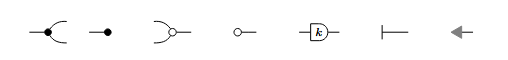
\includegraphics[width=1\linewidth]{images/GQA/GQA.png}
\end{figure}

\medskip

$\Sigma$-terms are defined by vertical and horizontal composition of terms with matching arity and coarity, and are modularized by $E$:

\begin{figure}[H]
    \centering
    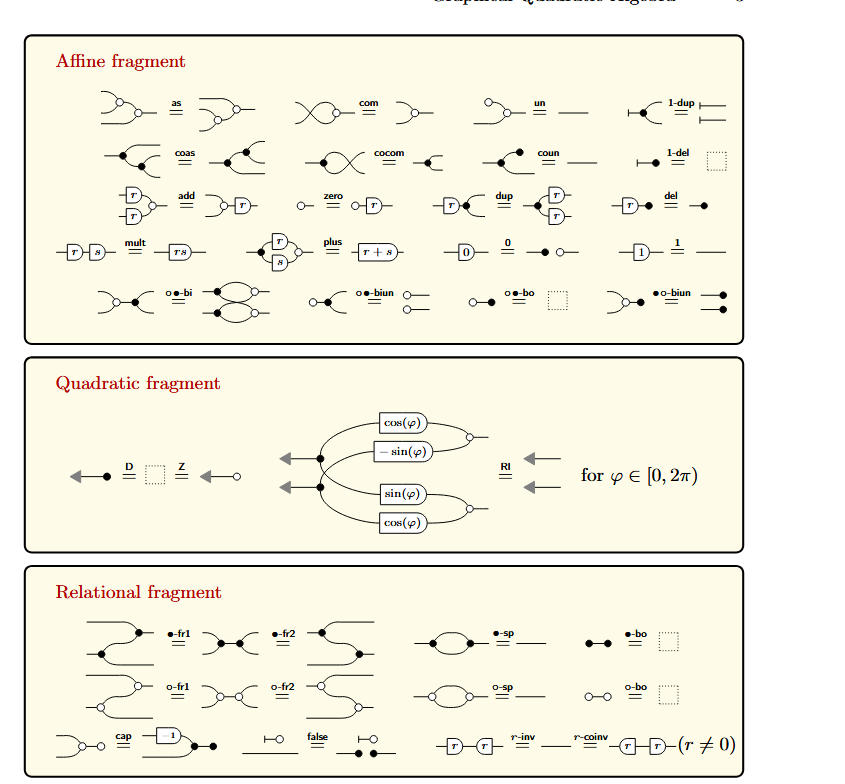
\includegraphics[width=1\linewidth]{images/GQA/GQAAxioms.png}
\end{figure}

The pair $(\Sigma,E)$ defines the symmetric monoidal theory generated by
the operators $\Sigma$ subject to the equations $E$.

We will define the interpretation functor $[ -]$, i.e., the semantics of each generator, as follows:

\begin{figure}[H]
    \centering
    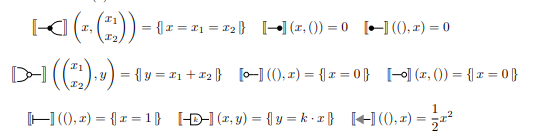
\includegraphics[width=1\linewidth]{images//GQA/GQAInterpretation.png}
\end{figure}

The interpretation of any $\Sigma$-term is, therefore, the vertical(tensor product) and horizontal(categorical composition) combination of the interpretation of each generator that composes it.
\end{definition}

Thus, \textbf{GQA} is an extension of the previous algebra for affine relations \textbf{GAA}.
The extension is done through the addition of a new generator, the gray arrow generator, and its associated axioms.
This is of particular interest, because is the interpretation of such generator
that is lifting the category to the level of weighted relations instead of binary relations.

To understand its role, recall that every generator of $\mathbf{GAA}$ is  interpreted
as the indicator function of some affine subspace. In this  picture, one may think of
numbers flowing along the wires, and each diagram  as encoding membership in some affine set.
The gray arrow  generator behaves differently, rather than enforcing a constraint on the
values running through the wire, it \emph{measures} them and produces a  real-valued output.
No number is transformed inside it; instead, a cost is  emitted.

A useful analogy comes from Electronics.
An electric circuit diagram is a formal diagram that allows you to represent an electric
circuit with wires and devices attached to those wires. In general,
what you see is current running in the wires and some components along it that alter the current. However,
one may attach a measurement device, like an ammeter, in the circuit.
That does not change the current, but it measures it, and outputs a number to outside the diagram.

Distinctively, the syntax admits an alternative probabilistic interpretation.
Under this reading, the gray arrow generator encodes the information of a Gaussian distribution
with mean 0,
its semmantics being that of the function $(\bullet, x)  \mapsto \mathcal{N}(0,x)$; categorically
this encodes the notion of a state in Markov Categories \cite{stein2023gaussian,Cho_2019, fritz2020synthetic}. Hence, \textbf{GQA}
expresses linear functions of random variables, more precisely of normally distributed random variables,
algebraically, turning composition into the act of probabilistic conditioning.

This interpretation of the syntax alludes to the understanding of the new added
generator as the act of observing a particular random variable, thus getting a number out of it.
Although such an extension is not explored in this work, we encourage the interested reader to pursue this
direction \cite{stein2024gqa,stein2025compositional}. We believe there exists a very strong interconnection between
the algebraic semmantics of optimization and that of probabilistic programming \cite{stein2024compositional}, the notion
of measuring in the convex setting being equivalent to that of observing the value of a random variable
in the stochastic one, and the composition playing the role of variable elimination in the first and
of conditioning in the latter. This lacks formality however, and we leave it to future works.

This provides a very meaningful intuition on how to interpret the new generator.
Rather then transforming the values carrieds by wires, the grey arrow generator measures
them and emits a real-valued cost. In this case,
the semantics of the diagram is $(x, \bullet) \mapsto \frac{1}{2}\|x\|^2$,
it measures the l2 norm of the number in the wires. This observation is central, since
the idea of a generator that "measures" or to "outputs" values carried by wires
is the conceptional foundation in our theory of Linear Programming develop in Section~\ref{sec:glp}.

Taking all the $\Sigma$-terms and quotient by their axioms $E$ we generate the free PROP of quadratic diagrams.

\begin{definition}[The Free category of quadratic diagrams]
    We call $\text{FreeP}_{\textbf{GQA}}$ the category of string diagrams of $\textbf{GQA}$
\end{definition}

Observe that we have associated to each generator of $\Sigma$ a visual  diagram. This can be made precise through the notion of a  \emph{strict monoidal functor}. Concretely, the Joyal--Street coherence  theorem \cite{joyal1991geometry} provides a canonical isomorphism of  categories
\[
  \mathbf{FreeP}_{\mathbf{GQA}} \;\xrightarrow{\;\sim\;}\; \mathbf{Diag}(\Sigma),
\]
where $\mathbf{Diag}(\Sigma)$ is the category of isotopy classes of  string diagrams generated by $\Sigma$. Under this isomorphism, each  generating morphism $g \in \Sigma$ is sent to the box labelled $g$ with  its input and output wires, composition $\circ$ is sent to vertical  stacking of diagrams, and the tensor product $\otimes$ is sent to  horizontal juxtaposition. The fact that this assignment is a  \emph{functor} is precisely what guarantees that diagrammatic reasoning  is sound: any equation derivable from the axioms of $\mathbf{GQA}$  holds if and only if the corresponding diagrams are related by  isotopy.

With the syntax in place, we now construct the corresponding semantic  category. As established in the preceding section, the objects of interest  are non-negative partial quadratic functions, or equivalently, quadratic  optimization problems with equality constraints whose objective is bounded  below by zero. These are encoded as \emph{quadratic relations} where $x \in \mathbb{R}^n $ is related to $y \in \mathbb{R}^m$ through a partial non-negative quadratic function
\[
f : \mathbb{R}^n \times \mathbb{R}^m \to [0,+\infty],
\]
where $f(x,y)$ is interpreted as the quadratic cost associated to the pair
$(x,y)$, with $f(x,y) = +\infty$ indicating infeasibility. The following definition constructs the categorical equivalent of such notion.

\begin{definition}[$\mathbf{QuadRel}$]

We define $\mathbf{QuadRel}$ as follows.

\medskip

\noindent
\textbf{Objects.}
Objects are natural numbers $n \in \mathbb{N}$, interpreted as the
Euclidean space $\mathbb{R}^n$.

\medskip

\noindent
\textbf{Morphisms.}
A morphism
\[
f : n \to m
\]
is a partial non-negative quadratic function

\medskip

\noindent
\textbf{Composition.}
Given
\[
f : n \to m,
\qquad
g : m \to k,
\]
their composite
\[
g \circ f : n \to k
\]
is defined by partial minimisation:
\[
(g \circ f)(x,z)
=
\inf_{y \in \mathbb{R}^m}
\left(
f(x,y) + g(y,z)
\right).
\]

\medskip

\noindent
\textbf{Identities.}
For each $n$, the identity morphism
\[
\mathrm{id}_n : n \to n
\]
is given by the quadratic form
\[
\mathrm{id}_n(x,y) =
\begin{cases}
0 & \text{if } x=y, \\
+\infty & \text{otherwise}.
\end{cases}
\]

\medskip

\noindent
\textbf{Monoidal structure.}
The tensor product on objects is addition:
\[
n \otimes m := n+m.
\]

For morphisms
\[
f : n_1 \to m_1,
\qquad
g : n_2 \to m_2,
\]
their tensor product
\[
f \otimes g : n_1+n_2 \to m_1+m_2
\]
is defined by
\[
(f \otimes g)(x_1,x_2,y_1,y_2)
=
f(x_1,y_1) + g(x_2,y_2).
\]

\medskip

From Proposition \ref{prop:partial quadratic composition}, composition is well defined. With these operations, $\mathbf{QuadRel}$ forms a symmetric monoidal
category (indeed a PROP).

\end{definition}

To prove that $\mathbf{GQA}$ presents $\mathbf{QuadRel}$, we require  several preliminary results. A central ingredient in completeness proofs  of this kind is the existence of a \emph{normal form}: a canonical  diagrammatic representation to which every morphism in the category can  be reduced by applying the axioms of the algebra.

The structure of the normal form is typically guided by the key  computational primitive of the semantic category in question. For example,  in $\mathbf{GLA}$, every linear relation can be represented by a pair of  matrices $A, B$ such that
\[
(x,y) \in R
\iff
Ax = By
\iff
[A \;-B] \begin{bmatrix} x \\ y \end{bmatrix} = 0
\iff
\widetilde{A}\,\widetilde{x} = 0,
\]
and the reduction to normal form proceeds through a diagrammatic argument  that mirrors Gaussian elimination on the underlying linear system.

In the quadratic setting, the analogous role is played by the
$QR$  factorization.
Just as Gaussian elimination reduces a linear relation to  a
canonical matrix kernel form, $QR$ factorization reduces a
quadratic  diagram to a canonical form by orthogonally decomposing the underlying  matrix.
This is the appropriate primitive because the objective function  $\|y\|^2$
is invariant under orthogonal transformations, so the axioms  of $\mathbf{GQA}$
can simulate $QR$ steps diagrammatically. The following  results make this precise.

\begin{proposition}\label{prop:projection}
    If $S,D$ are complementary subspaces, then we can prove that:
    \begin{figure}[H]
        \centering
        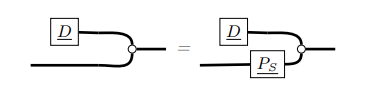
\includegraphics[width=1\linewidth]{images/GQA/subspaceProj.png}
    \end{figure}
\end{proposition}
\begin{proof}
    From the fact that $P_S + P_D = I$, such that $P_S, P_D$ are the projection matrices over
    subspaces $S$ and $D$, we show:

    \begin{figure}[H]
        \centering
        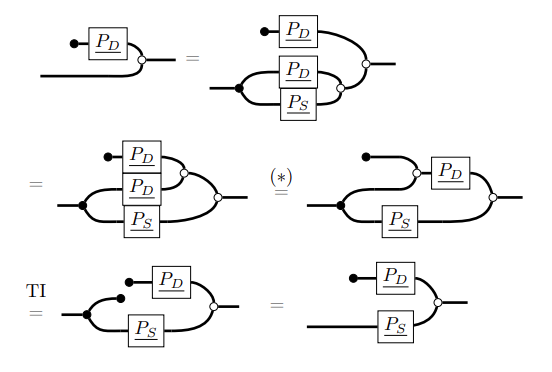
\includegraphics[width=1\linewidth]{images/GQA/ProofProjection.png}
    \end{figure}
\end{proof}

Above result is an analogous way of saying that:
$\{(x,y)|\exists z \in D, z+x =y \} = \{(x,y)|\exists z \in D, z = y - x\}$,
by the orthogonal unique decomposition theorem
$\{(x,y)|\exists z \in D, z = y - x_S - x_D \} = \{(x,y)|\exists z \in D, z + x_D = y - x_S\}$
Since $x_D,z \in D \implies x_D + z = \tilde{z} \in D$ and, by the uniqueness of the decomposition,
$y = \tilde{z} + x_S \implies \tilde{z} = y_D, y_S = x_S$.
$\{(x,y)|\exists \tilde{z} \in D, \tilde{z} = y - x_S\}$.
Visually, one can interpret above diagram as the idea that summing a dangling wire with a
subspace $D$ is equivalent to ask for a pair $(y_{D^\perp}, y)$.

The following remmark establishes a preliminary normal form for the
directed fragment $\overrightarrow{\mathbf{GQA}}$, which will serve as
the key stepping stone toward the full normal form theorem. Intuitively,
it says that any diagram in this fragment can be reorganised into a
canonical block structure determined by a subspace $S$ and compatible
matrix data.

\begin{remark}\label{rmk:normalformgqa}
    Let $M$ be any diagram generated by the fragment
    $\overrightarrow{\mathbf{GQA}}$ (recall Definition~\ref{def:arrows})
    together with the generator $\bullet-$. By collecting terms, we can
    write it as a diagram of the form
    \begin{figure}[H]
        \centering
        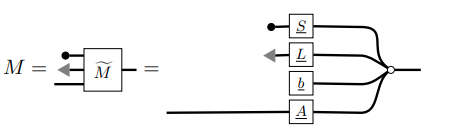
\includegraphics[width=1\linewidth]{images//GQA/GQAeNormalForm.png}
    \end{figure}
    such that $S \subseteq \mathbb{R}^n$ is a vector subspace,
    $b \in S^\perp$, $\operatorname{im}(LL^\top) \subseteq S^\perp$,
    and $\operatorname{im}(A) \subseteq S^\perp$(By Proposition~\ref{prop:projection}).
\end{remark}

\begin{proposition}\label{prop:quadrel_equiv}
Let $N$ be a diagram in the followinf form
    \begin{figure}[H]
        \centering
        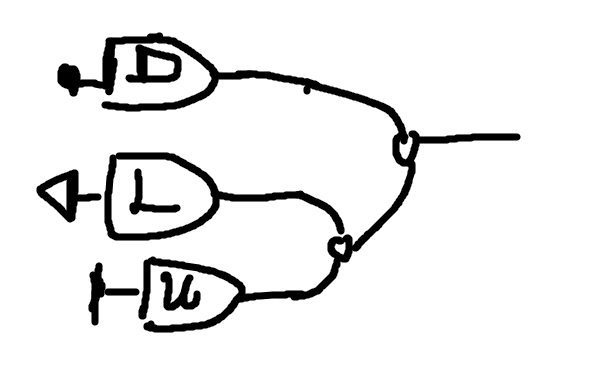
\includegraphics[width=1\linewidth]{images//GQA/preliminary form.png}
    \end{figure}
with data $(D, \mu, L)$, where
$D \subseteq \mathbb{R}^n$ is a vector subspace, $\mu \in D^\perp$,
$L$ is a lower-triangular matrix with
and $\operatorname{im}(LL^\top) \subseteq D^\perp$.
Its semantic interpretation in $\mathbf{QuadRel}$ is the partial
non-negative quadratic function
\[
[N](x)
= \tfrac{1}{2}(x - \mu)^\top L L^\top (x - \mu) + \{|D^\perp + \mu|\}(x),
\]
Moreover, two canonical block-form diagrams $N_1$, $N_2$ with data
$(D_1, \mu_1, L_1)$ and $(D_2, \mu_2, L_2)$ satisfy
$[N_1] = [N_2]$ in $\mathbf{QuadRel}$ if and only if
\[
D_1 = D_2, \qquad \mu_1 = \mu_2, \qquad L_1 L_1^\top = L_2 L_2^\top.
\]
\end{proposition}

\begin{proof}
The first claim follows by direct computation of the interpretation
functor $[-]$ applied to the block form. The $L$-block contributes
the quadratic term $\tfrac{1}{2}(x-\mu)^\top LL^\top(x-\mu)$, the
subspace $D$ contributes the indicator $\iota_{D^\perp}$, and the
vector $\mu$ shifts the centre of the feasible region.

For the equivalence, the $(\Leftarrow)$ direction is immediate from
the first claim. For $(\Rightarrow)$, suppose $[N_1] = [N_2]$
pointwise on $\mathbb{R}^n$.

The domain of finiteness of $[N_i]$ is the affine subspace
$D_i^\perp + \mu_i$. Since $[N_1] = [N_2]$, these domains coincide:
$D_1^\perp + \mu_1 = D_2^\perp + \mu_2$. Two cosets are equal only
if their direction subspaces agree, so $D_1^\perp = D_2^\perp$,
hence $D_1 = D_2$. Write $D := D_1 = D_2$.

The coset equality now gives $\mu_1 - \mu_2 \in D^\perp$.
Evaluating both functions at $x = \mu_1$:
\[
0 = [N_1](\mu_1) = [N_2](\mu_1)
  = \tfrac{1}{2}(\mu_1 - \mu_2)^\top L_2 L_2^\top (\mu_1 - \mu_2).
\]
Since $L_2 L_2^\top$ is positive semidefinite and its restriction to
$D^\perp$ is positive definite (as $\operatorname{im}(L_2 L_2^\top)
\subseteq D^\perp$ with $L_2$ of full rank on $D^\perp$), the
equation above forces $\mu_1 - \mu_2 = 0$, i.e.\ $\mu_1 = \mu_2$.

With $D_1 = D_2$ and $\mu_1 = \mu_2 =: \mu$ established, the identity
$[N_1](x) = [N_2](x)$ for all $x \in D^\perp + \mu$ yields
\[
(x - \mu)^\top L_1 L_1^\top (x - \mu)
= (x - \mu)^\top L_2 L_2^\top (x - \mu)
\qquad \forall\, x \in D^\perp + \mu.
\]
Setting $v = x - \mu \in D^\perp$, this is a quadratic identity on
$D^\perp$. By polarisation it implies $L_1 L_1^\top = L_2 L_2^\top$
as operators on $D^\perp$, and since both sides vanish on $D$, equality
holds on all of $\mathbb{R}^n$.
\end{proof}

We now state and prove the main normal form theorem for $\mathbf{GQA}$.
The theorem states that every
diagram can be decomposed into a purely relational part — a morphism in
$\mathbf{GQA}$ — and a non-negative scalar, corresponding respectively to
the constraint structure and the quadratic cost of the underlying
optimization problem. The proof proceeds by a diagrammatic version of
$QR$ factorization: orthogonal transformations are simulated by axiom
applications, progressively eliminating generators until the canonical
form is reached.

\begin{theorem}[\textbf{GQA} Normal Form]
    Every diagram $M \in \overrightarrow{\mathbf{GQA}}$ can be rewritten,
    modulo the axioms $E$, as $M' \otimes c$ where $M' \in \mathbf{GQA}$
    and $c \in [0,+\infty]$ is a scalar of the form:
    \begin{figure}[H]
        \centering
        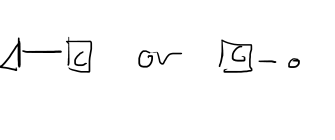
\includegraphics[width=.75\linewidth]{images//GQA/NormalFormScalar.png}
    \end{figure}
\end{theorem}

\begin{proof}
    In a hypergraph category, there is a bijection between
    $\mathrm{Hom}(c,d)$ and $\mathrm{Hom}(\mathbb{1}, c \otimes d)$,
    where $\mathbb{1}$ is the monoidal unit. Diagrammatically, this
    corresponds to bending wires from the left side to the right using
    the cap and cup morphisms of the compact closed structure:
    \begin{figure}[H]
        \centering
        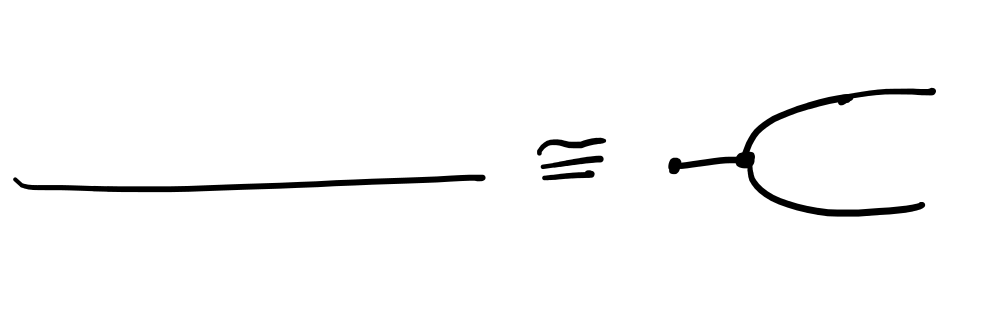
\includegraphics[width=1\linewidth]{images/States.png}
    \end{figure}
    Morphisms from the monoidal unit are called \emph{states}. This
    means that any diagram can be reorganised so that all dangling wires
    appear on one side. Collecting all dangling wires to the left and all
    generators that are morphisms from the unit object to the right, we
    obtain a diagram of the form:
    \begin{figure}[H]
        \centering
        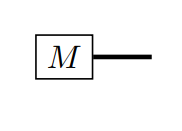
\includegraphics[width=.3\linewidth]{images//GQA/CollectDiagrams.png}
    \end{figure}
    where $M$ is a diagram of arity $0$. We now separate the $-\circ$
    generators from the remaining ones, and collect the dangling wires
    accordingly. Without loss of generality, assume there are $K$ such
    generators:
    \begin{figure}[H]
        \centering
        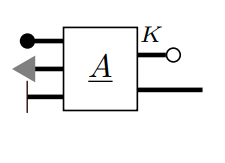
\includegraphics[width=.3\linewidth]{images//GQA/ProofNormalForm1.png}
    \end{figure}
    Here $A$ is a fragment of $\overrightarrow{\mathbf{GLA}}$ and
    therefore represents a matrix \cite{bonchi2017interacting}. To realize this, just recall that we can take the co-sum and co-copy and transform them into the copy and the sum by bending the wires with a spider.

    Applying the axioms, we derive:
    \begin{figure}[H]
        \centering
        
\includegraphics[width=1\linewidth]{images//GQA/ProofNormalForm2.png}
    \end{figure}
    We use the fact that a matrix can be decomposed into rows. We
    pick $A_1$ as the row satisfying $A_1 x = 0$ and decompose it
    into scalar components $\alpha, \beta, \gamma$ — one-dimensional
    row vectors — such that $\alpha x_1 + \beta x_2 + \gamma x_3 = 0$.
    If $\beta = 0$, the corresponding black dot generator is eliminated
    immediately:
    \begin{figure}[H]
        \centering
        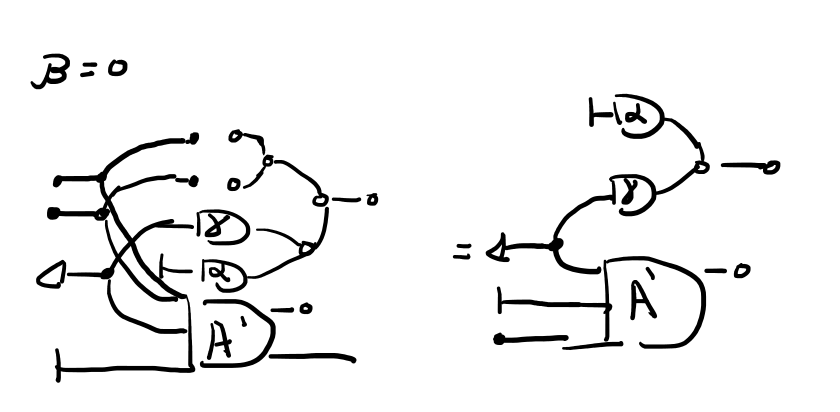
\includegraphics[width=1\linewidth]{images//GQA/ProofNormalForm3.png}
    \end{figure}
    If $\beta \neq 0$, then there exists an index $i$ such that
    $\beta_i \neq 0$, and we can eliminate one occurrence of the white
    dot and one of the black dot simultaneously:
    \begin{figure}[H]
        \centering
        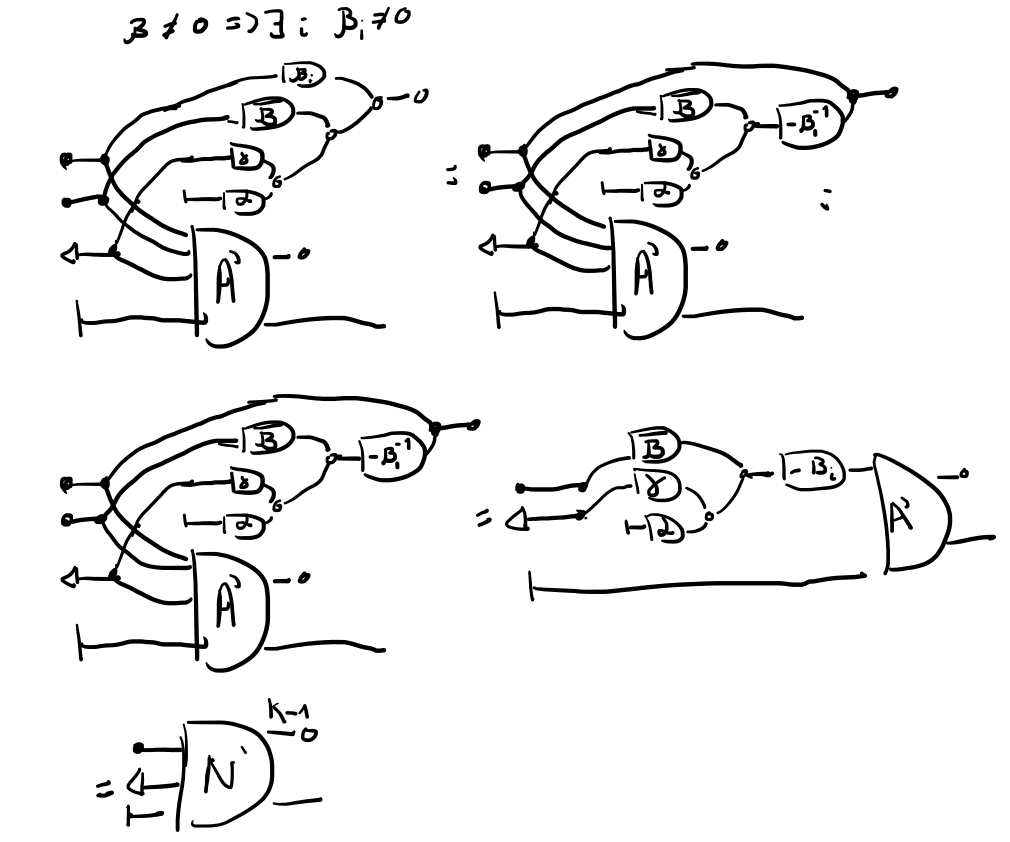
\includegraphics[width=1\linewidth]{images//GQA/ProofNormalForm4.png}
    \end{figure}
    By induction on the number of rows, we repeat this process for all
    rows with $\beta \neq 0$, leaving only rows with $\beta = 0$. The
    diagram reduces to:
    \begin{figure}[H]
        \centering
        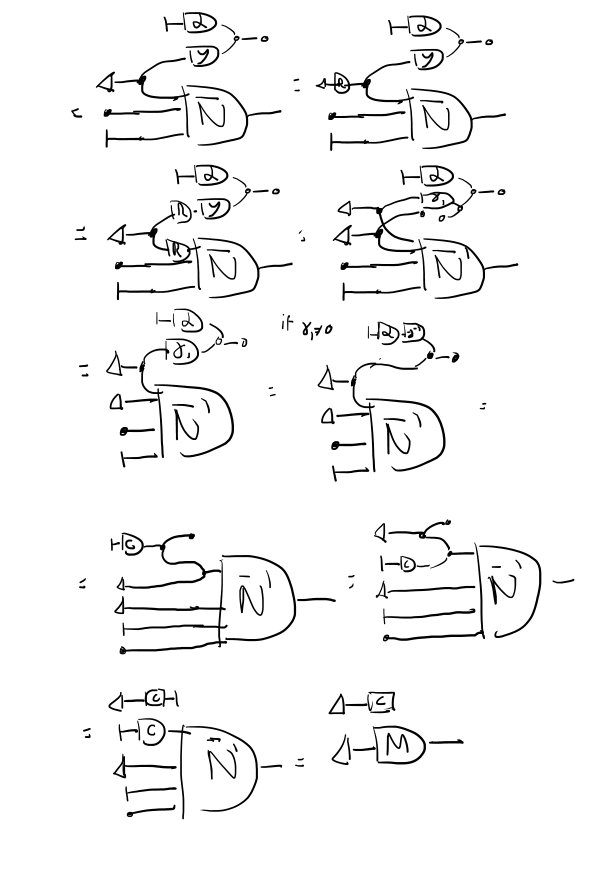
\includegraphics[width=1\linewidth]{images//GQA/ProofNormalForm5.png}
    \end{figure}
    Here $R$ is an orthogonal matrix such that
    $R\gamma = (\gamma_1, 0, \ldots, 0)$. If $\gamma_1 \neq 0$, the
    normal form is achieved. If $\gamma_1 = 0$, the wire disconnects
    trivially and we are left with:
    \begin{figure}[H]
        \centering
        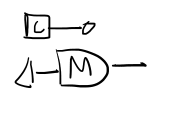
\includegraphics[width=.5\linewidth]{images//GQA/ProofNormalForm6.png}
    \end{figure}
    In both cases the diagram has been reduced to the claimed normal form
    $M' \otimes c$, completing the proof.
\end{proof}

With the normal form established, we now have all the ingredients needed
to prove the three properties — soundness, expressivity, and completeness
— that together guarantee that $\mathbf{GQA}$ is a faithful and complete
axiomatisation of $\mathbf{QuadRel}$. We treat each in turn.

\begin{lemma}[Soundness]
   If $s = t$ in $\mathrm{FreeP}_{\mathbf{GQA}}$, then $[s] = [t]$
   in $\mathbf{QuadRel}$.
\end{lemma}

\begin{proof}
    Since $\mathbf{AffRel}$ embeds into $\mathbf{QuadRel}$ via the
    indicator function, all axioms inherited from $\mathbf{GAA}$ are
    already sound in $\mathbf{QuadRel}$. It therefore suffices to verify
    soundness for the newly introduced axioms involving the gray arrow
    generator, which is done by direct computation of the corresponding
    semantic interpretations:
    \begin{figure}[H]
        \centering
        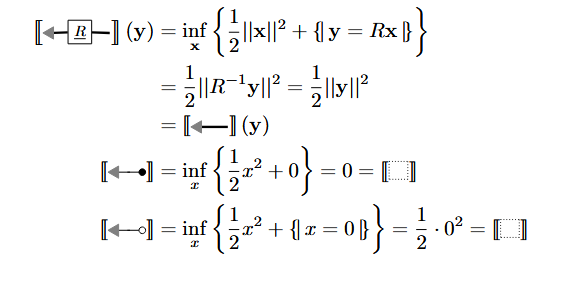
\includegraphics[width=1\linewidth]{images//GQA/SoundnessGQA.png}
    \end{figure}
\end{proof}

\begin{lemma}[Expressivity]
    For every $f : m \to n$ in $\mathbf{QuadRel}$, there exists a
    $\Sigma$-term $s : m \to n$, equivalently a morphism
    $s \in \mathrm{Hom}_{\mathrm{FreeP}_{\mathbf{GQA}}}(m,n)$,
    such that $[s] = f$.
\end{lemma}

\begin{proof}
    By Proposition~\ref{prop:PQFEquivalence}, for every non-negative
    partial quadratic function $f$ there exists an invertible coordinate
    change $g$ such that
    \[
    g(f(x_1, x_2, x_3))
    = \tfrac{1}{2}\|x_1\|^2 + \mathbf{1}_{\{0\}}(x_3),
    \]
    which is represented diagrammatically as:
    \begin{figure}[H]
        \centering
        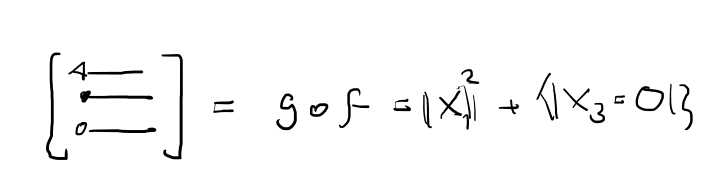
\includegraphics[width=1\linewidth]{images/GQA/PQFDiagram.png}
    \end{figure}
    Since the coordinate change $g$ is itself expressible as a morphism
    in $\mathbf{GQA}$, the general case follows by composition:
    \begin{figure}[H]
        \centering
        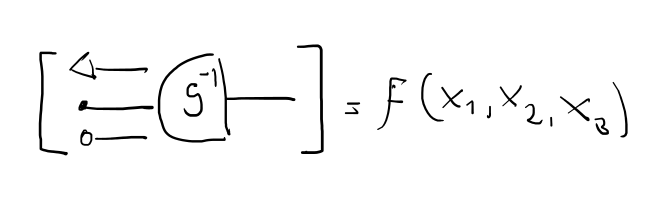
\includegraphics[width=1\linewidth]{images//GQA/ProofExpressivity.png}
    \end{figure}
\end{proof}

\begin{lemma}[Completeness]
   If $[s] = [t]$ in $\mathbf{QuadRel}$, then $s = t$ in
   $\mathrm{FreeP}_{\mathbf{GQA}}$.
\end{lemma}

\begin{proof}
    We reduce both $s$ and $t$ to their respective normal forms
    $s = M_1 \otimes c_1$ and $t = M_2 \otimes c_2$ using the Normal
    Form Theorem. Since $M_1, M_2$ lie in the fragment
    $\overrightarrow{\mathbf{GQA}} \cup \{\bullet{-}\}$,
    Lemma~\ref{rmk:normalformgqa} allows us to write them in the
    canonical block form:
    \begin{figure}[H]
        \centering
        
\includegraphics[width=0.25\linewidth]{images//GQA/ProofCompleteness1.png}
    \end{figure}
    where $D_i$ is a vector subspace, $\mu_i \in D_i^\perp$, $L_i$ is
    lower triangular, and $\operatorname{im}(L_i L_i^\top) \subseteq
    D_i^\perp$. By Proposition~\ref{prop:quadrel_equiv}, $[N_1] = [N_2]$
    if and only if $D_1 = D_2$, $\mu_1 = \mu_2$, and
    $L_1 L_1^\top = L_2 L_2^\top$.

    If $AA^\top = BB^\top$, then there exists an orthogonal matrix $R$
    such that $A = BR$, and the axioms of $\mathbf{GQA}$ allow us to
    rewrite one diagram into the other by applying the corresponding
    orthogonal transformation diagrammatically. Appealing to the
    completeness of $\mathbf{GAA}$ for the affine fragment, we conclude
    $N_1 = N_2$ in $\mathrm{FreeP}_{\mathbf{GQA}}$. Since
    $M_i = N_i \otimes c_i$ and $c_1 = c_2$ follows from
    $[s] = [t]$, we obtain $M_1 = M_2$, as desired.
\end{proof}

Combining the three lemmas, the main presentation theorem follows
immediately.

\begin{theorem}
    $\mathbf{QuadRel}$ is presented by $\mathrm{FreeP}_{\mathbf{GQA}}$.
\end{theorem}

\begin{proof}
    Soundness, expressivity, and completeness were established by the
    preceding three lemmas. Together they imply that the canonical PROP
    morphism $\mathrm{FreeP}_{\mathbf{GQA}} \to \mathbf{QuadRel}$ is
    full, faithful, and essentially surjective, hence an isomorphism of
    PROPs.
\end{proof}

\subsection{Results in GQA}

Having established that $\mathbf{GQA}$ completely axiomatises
$\mathbf{QuadRel}$, we now demonstrate the expressive power of the
calculus by deriving several non-trivial results purely through string
diagram manipulation. These propositions illustrate that the diagrammatic
language is not merely a notational device, but a genuine proof calculus
in which geometric and algebraic arguments about quadratic optimization
can be carried out compositionally. We begin with two fundamental
structural results — the expansion and contraction relations — before
moving to orthogonal projections and the generalized singular value
decomposition.

\begin{proposition}[Expansion Relation]
\leavevmode\par
\noindent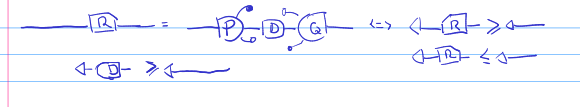
\includegraphics[width=\linewidth]{images/GQA/ExpansionRelation.png}
\end{proposition}

\begin{proof}
\leavevmode\par
\noindent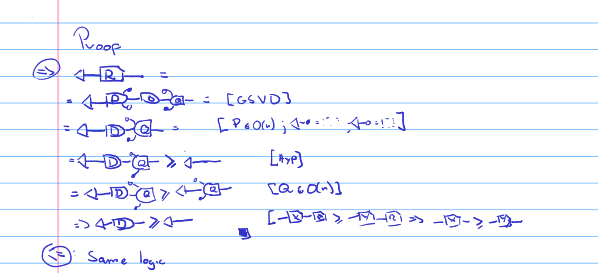
\includegraphics[width=\linewidth]{images/GQA/ProofExpansion.png}
\end{proof}

\begin{proposition}[Contraction Relation]
\leavevmode\par
\noindent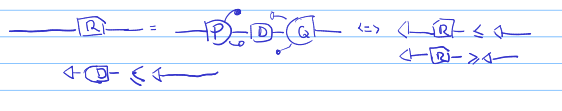
\includegraphics[width=\linewidth]{images/GQA/ContractionRelation.png}
\end{proposition}

\begin{proof}
    The proof follows by an entirely analogous diagrammatic argument to
    that of the Expansion Relation above, applying the axioms of
    $\mathbf{GQA}$ in the reverse direction.
\end{proof}

The following proposition establishes the diagrammatic representation of
orthogonal projections. This is a key result, as projections appear
naturally in least-squares problems whenever the system $Ax = b$ is
inconsistent, and the pseudoinverse computation relies essentially on
projecting onto the image of $A$.

\begin{proposition}[Matrix Projection]
    If $P$ is an orthogonal projection, then:
\leavevmode\par
\noindent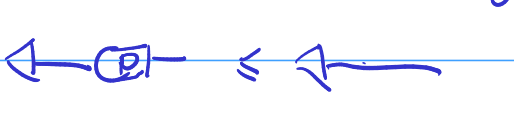
\includegraphics[width=\linewidth]{images/GQA/OrthogonalProj.png}
\end{proposition}

\begin{proof}
\leavevmode\par
\noindent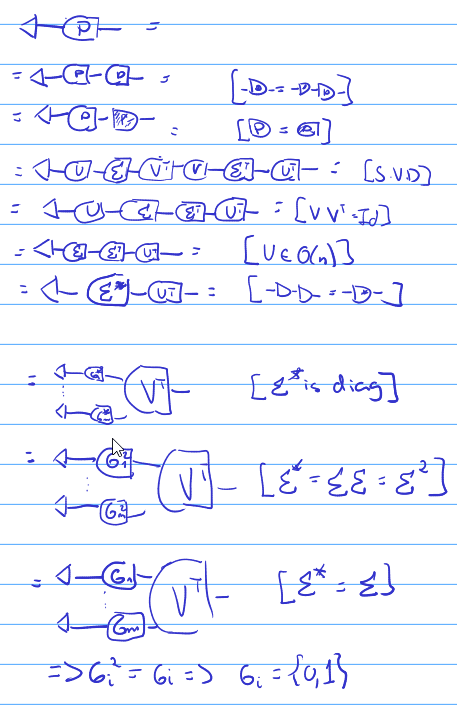
\includegraphics[width=\linewidth]{images/GQA/ProofMatrixProj.png}
\noindent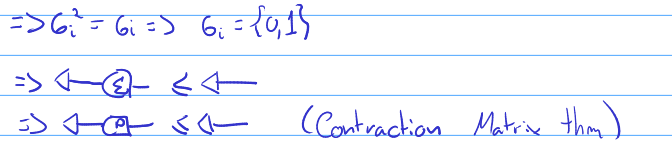
\includegraphics[width=\linewidth]{images/GQA/ProofMatrixProj2.png}
\end{proof}

The next result extends the orthogonality argument to the setting of
generalized singular value decompositions.

\begin{proposition}[GSVD Orthogonality]
\leavevmode\par
\noindent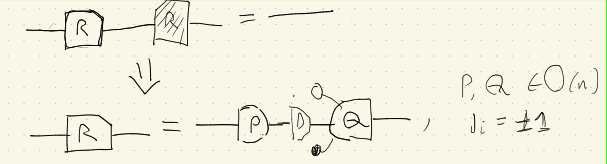
\includegraphics[width=\linewidth]{images/GQA/GSVDOrth.png}
\end{proposition}

\begin{proof}
\leavevmode\par
\noindent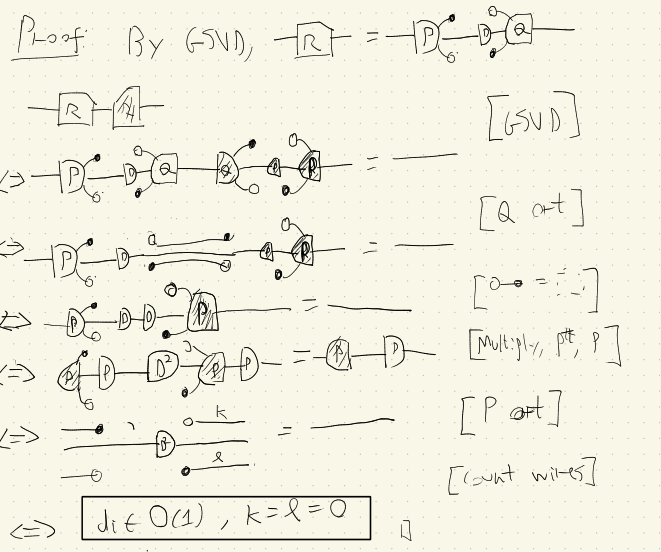
\includegraphics[width=\linewidth]{images/GQA/ProofGSVDOrth.png}
\end{proof}

Finally, the Relation Projection proposition combines the preceding
results to characterise how orthogonal projections interact with
quadratic relations.

\begin{proposition}[Relation Projection]
\leavevmode\par
\noindent
\includegraphics[width=\linewidth]{images/GQA/OrthogonalProjectionRelation.png}
\noindent
\includegraphics[width=\linewidth]{images/GQA/OrthogonalProjRel2.png}
\end{proposition}

\begin{proof}
\leavevmode\par
\noindent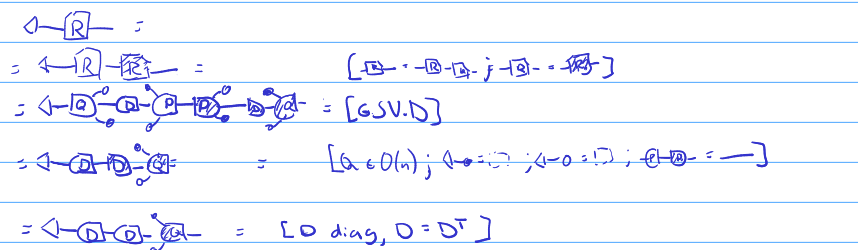
\includegraphics[width=\linewidth]{images/GQA/ProofOrthRel.png}
\noindent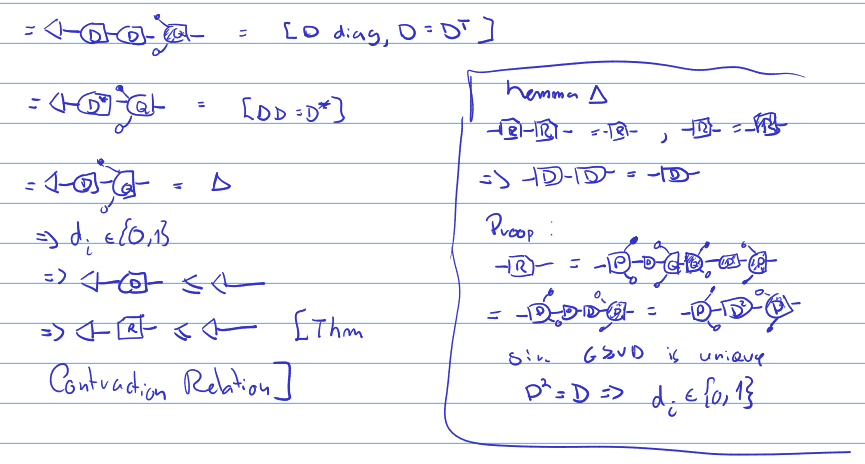
\includegraphics[width=\linewidth]{images/GQA/ProofOrthRel2.png}
\end{proof}
\begin{proposition}[The OLS estimator]

\end{proposition}
\section{Polyhedral Relations}

While the previous section treated quadratic costs, we now
turn to a combinatorially richer class of objects: polyhedra and polyhedral
cones. These are the fundamental geometric structures underlying linear
programming, and they admit a categorical treatment entirely analogous to
the one developed for quadratic relations. The key difference is that
composition here is governed by Fourier-Motzkin Elimination (FME) rather
than $QR$ factorization: projecting a polyhedron onto a subspace is
precisely variable elimination, and it is this operation that categorical
composition will simulate diagrammatically.

Unlike the previous section, the theory developed here remains
a within  the category of binary relations since morphisms are still indicator functions
of subsets of $\mathbb{R}^n \times \mathbb{R}^m$, encoding feasibility
constraints rather than objective functions. In this sense, $\mathbf{GPA}$
does not yet enter the weighted relational world of not being able to express more meaningful
optimization problems. This is nonetheless a critical step in the development.
Axiomatizing linear inequality constraints diagrammatically,  $\mathbf{GPA}$ provides
the Symmetric Monoidal Inequality Theory (SMIT)~\cite{bonchi2021polyhedral}  that will
serve as the structural foundation for our final contribution,  $\mathbf{GLP}$,
where these constraints are combined with a linear objective to form full parametric linear programs.

We begin by recalling the standard definitions of polyhedral cones and
polyhedra, before introducing the two graphical algebras of
$\mathbf{GPA}_{\rtop}$ \cite{bonchi2021polyhedral} for polyhedral cones and $\mathbf{GPA}$ for
general polyhedra, proving that each completely axiomatises its
corresponding semantic category.

\begin{definition}\label{def:pcform}
A set $C \subseteq \mathbb{R}^n$ is called a \emph{polyhedral cone} if
there exists a matrix $A \in \mathbb{R}^{m \times n}$ such that
\[
C = \{x \in \mathbb{R}^n \mid Ax \ge 0\}.
\]
\end{definition}

\begin{definition}\label{polyform}
A set $P \subseteq \mathbb{R}^n$ is called a \emph{polyhedron} if there
exist $A \in \mathbb{R}^{m \times n}$ and $b \in \mathbb{R}^m$ such that
\[
P = \{x \in \mathbb{R}^n \mid Ax \ge b\}.
\]
\end{definition}

Note that a polyhedral cone is a special case of a polyhedron with $b = 0$.
The distinction is algebraically significant: cones are closed under
non-negative scaling and admit a purely homogeneous representation, while
general polyhedra may be translated. This distinction is reflected in the
two graphical algebras we now define, where $\mathbf{GPA}_{\rtop}$ handles
the homogeneous case and $\mathbf{GPA}$ extends it with an affine generator.

\begin{definition}[Graphical Polyhedral Algebra]
    We call $\mathbf{GPA}$ the SMT generated by extending $\mathbf{GAA}$
    with the following generator and its semantics:
    \begin{figure}[H]
        \centering
        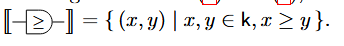
\includegraphics[width=0.7\linewidth]{images/GPA/PolyGen.png}
    \end{figure}
    along with the following additional equations:
    \begin{figure}[H]
        \centering
        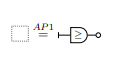
\includegraphics[width=0.2\linewidth]{images//GPA/AffineAxiom.png}
    \end{figure}
    \begin{figure}[H]
        \centering
        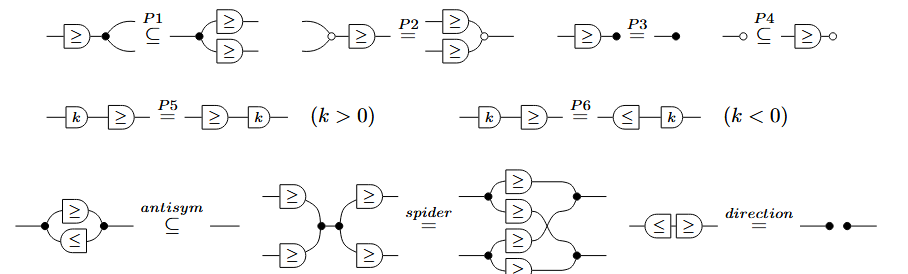
\includegraphics[width=1\linewidth]{images/GPA/PolyAxioms.png}
    \end{figure}
\end{definition}

\begin{definition}[Graphical Polyhedral Cones Algebra]
    We call $\mathbf{GPA}_{\rtop}$ the SMT generated by $\mathbf{GPA}$
    but excluding the affine generator $\rtop$ and its associated
    equations. This fragment axiomatises polyhedral cones, where no
    translation is present.
\end{definition}

\begin{definition}[The Free Categories of Polyhedral Diagrams]
    We call $\mathrm{FreeP}_{\mathbf{GPA}}$ the PROP freely generated
    by $\mathbf{GPA}$, and $\mathrm{FreeP}_{\mathbf{GPA}_{\rtop}}$ the
    PROP freely generated by $\mathbf{GPA}_{\rtop}$.
\end{definition}

We now define the two semantic categories that these algebras will be
shown to axiomatise. Just as $\mathbf{AffinRel}$ captured affine space as morphisms, the categories $\mathbf{PCRel}$ and
$\mathbf{PolyRel}$ capture polyhedral cones and polyhedra as morphisms,
with relational composition playing the role of variable elimination.

\begin{definition}[The prop $\mathbf{PCRel}$ of polyhedral cones]
Let $k$ be an ordered field, in this case the real numbers. The prop
$\mathbf{PCRel}_k$ is defined as follows:
\begin{itemize}
    \item Objects are natural numbers $n \in \mathbb{N}$, interpreted
    as the space $k^n$.
    \item A morphism $n \to m$ is a polyhedral cone
    $R \subseteq k^n \times k^m$
    for which there exist $p \in \mathbb{N}$ and
    $A \in k^{p \times (n+m)}$ such that
    \[
    R = \left\{ (x,y) \in k^n \times k^m \;\middle|\;
    A \begin{pmatrix} x \\ y \end{pmatrix} \ge 0 \right\}.
    \]
    \item Composition is relational composition.
    \item The monoidal product on objects is addition $n \otimes m := n+m$,
    and on morphisms is the Cartesian product.
\end{itemize}
\end{definition}

\begin{definition}[The prop $\mathbf{PolyRel}$ of polyhedra]
Let $k$ be an ordered field. The prop $\mathbf{PolyRel}_k$ is defined
as follows:
\begin{itemize}
    \item Objects are natural numbers $n \in \mathbb{N}$, interpreted
    as the space $k^n$.
    \item A morphism $n \to m$ is a polyhedron
    $R \subseteq k^n \times k^m$
    for which there exist $p \in \mathbb{N}$,
    $A \in k^{p \times (n+m)}$, and $b \in k^p$ such that
    \[
    R = \left\{ (x,y) \in k^n \times k^m \;\middle|\;
    A \begin{pmatrix} x \\ y \end{pmatrix} + b \ge 0 \right\}.
    \]
    \item Composition is relational composition.
    \item The monoidal product on objects is addition $n \otimes m := n+m$,
    and on morphisms is the Cartesian product.
\end{itemize}
\end{definition}

\subsection{The algebra \texorpdfstring{$\mathbf{GPA}_{\rtop}$}{GPA}
and \texorpdfstring{$\mathbf{PCRel}$}{PCRel}}

We now develop the presentation theory for the homogeneous case. The
central computational primitive here is Fourier--Motzkin Elimination,
which projects a polyhedral cone onto a lower-dimensional space by
eliminating one variable at a time.

To accomplish it, we need some previous results regarding small diagrammatic
operations. The first result we prove is the transitivity property of the
generator, i.e. $-\ge-\ge- = -\ge- $

\begin{figure}[H]
    \centering
    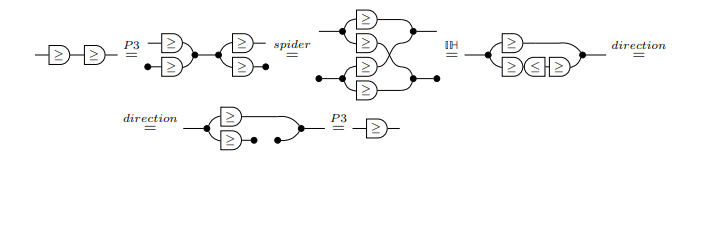
\includegraphics[width=1\linewidth]{images/GPA/transitivity.png}
\end{figure}

Next, we show that $\ge$ is reflexive

\begin{figure}[H]
    \centering
    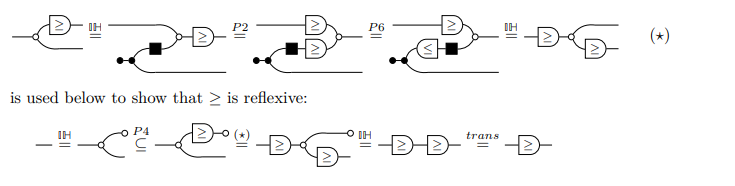
\includegraphics[width=1\linewidth]{images/GPA/reflexivity.png}
\end{figure}

and antisymetric

\begin{figure}[H]
    \centering
    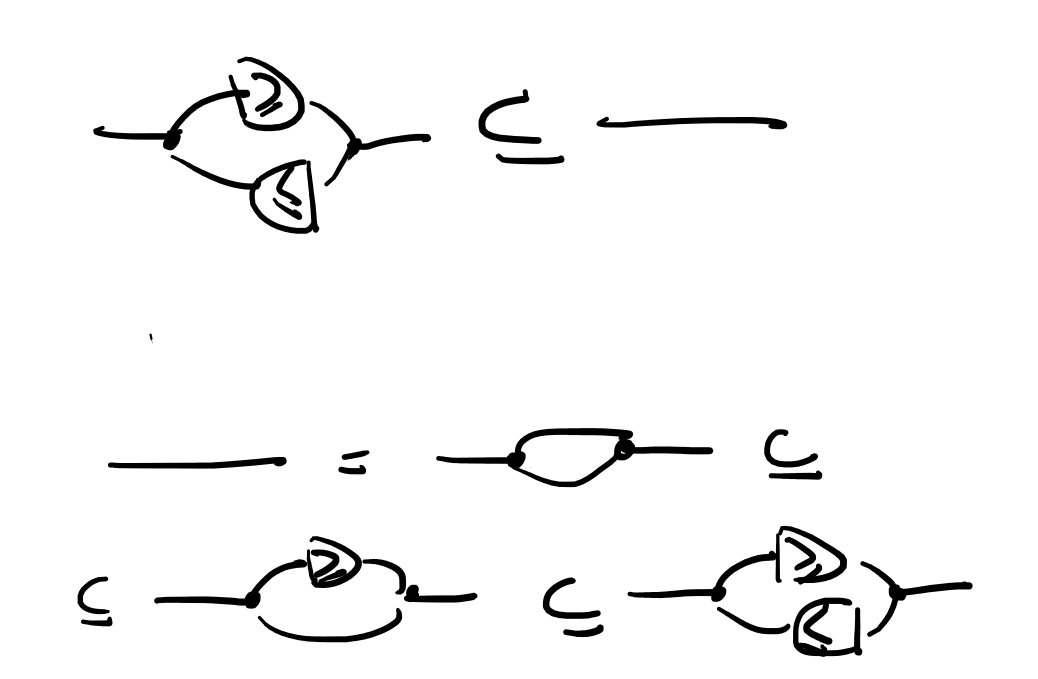
\includegraphics[width=1\linewidth]{images/GPA/antysim.png}
\end{figure}

With those results in places we are ready to prove the diagrammatic FME:

\begin{proposition}[Fourier-Motzkin Elimination]
The following diagrammatic procedure is equivalent to perform the FME
algorithm
\begin{figure}[H]
    \centering
    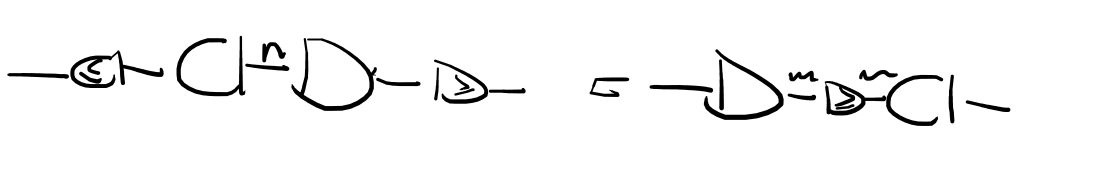
\includegraphics[width=1\linewidth]{images//GPA/FMEDiag.png}
\end{figure}
\end{proposition}

\begin{proof}
    The proof proceeds by induction on the number of inequalities.
    \begin{figure}[H]
        \centering
        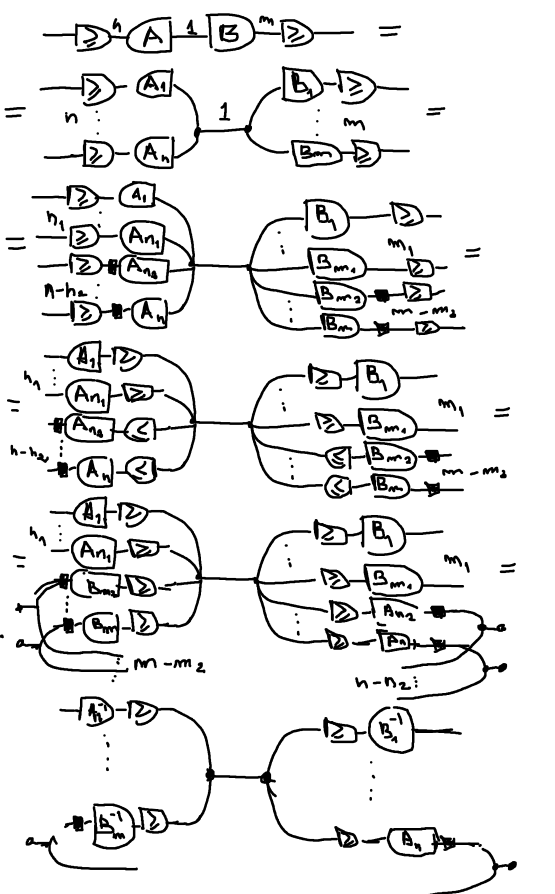
\includegraphics[width=1\linewidth]{images//GPA/ProofFMEDiag.png}
    \end{figure}
    \begin{figure}[H]
        \centering
        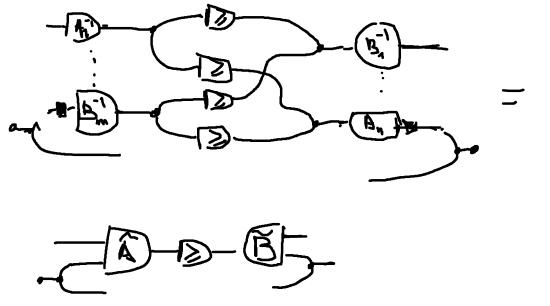
\includegraphics[width=1\linewidth]{images//GPA/ProofFMEDiag2.png}
    \end{figure}

    Now we show the inductive step for $n+1$:
\end{proof}

With FME available as a diagrammatic operation, we can now prove the
normal form theorem for $\mathbf{GPA}_{\rtop}$. We proceed by structural induction,
handling generators, composition, and tensor product in turn,
using FME  steps to push all inequality generators into a
canonical block form.

\begin{theorem}[First Normal Form]\label{thm:FirstNormalForm}
   Every diagram in $\mathbf{GPA}_{\rtop}$ admits an isomorphic representation,
   modulo the axioms, of the following form:
   \begin{figure}[H]
       \centering
       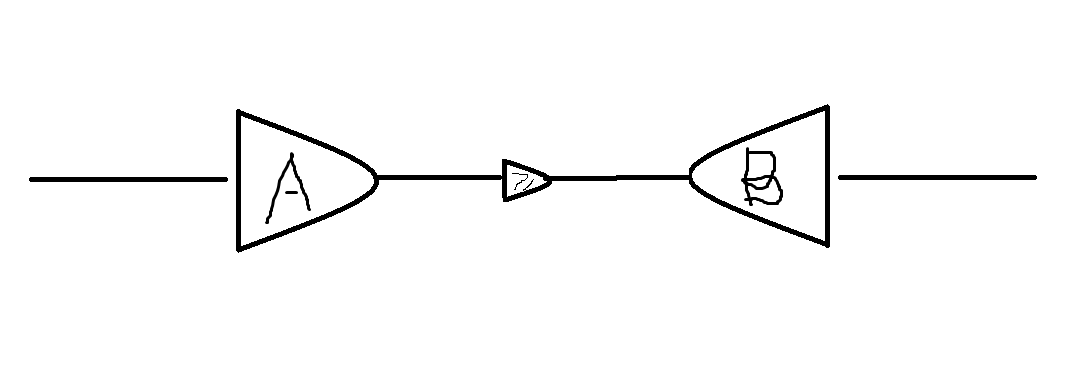
\includegraphics[width=0.75\linewidth]{images/GPA/FirstNormalFormPCRel.png}
   \end{figure}
\end{theorem}

\begin{proof}
    We proceed by structural induction. The two base cases are as follows.
    First, the $\ge$ generator:
    \begin{figure}[H]
        \centering
        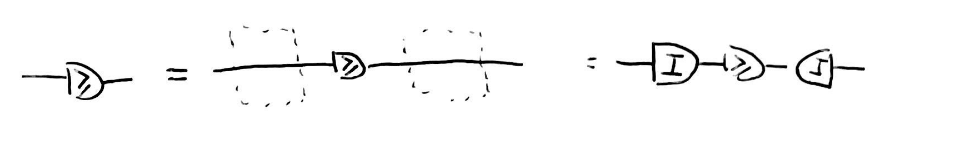
\includegraphics[width=.75\linewidth]{images//GPA/BaseCase1NormalFormProof.png}
    \end{figure}
    Second, for any diagram $c$ in $\mathbf{GLA}$:
    \begin{figure}[H]
        \centering
        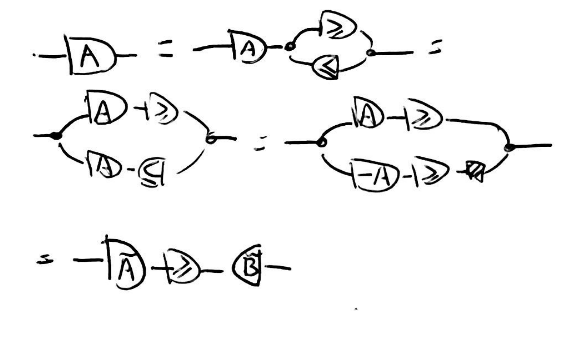
\includegraphics[width=1\linewidth]{images//GPA/BaseCase2NormalFormProof.png}
    \end{figure}
    For the inductive step, we consider composition of two diagrams
    $c; d$ in $\mathbf{GPA}_{\rtop}$. By the inductive hypothesis, both
    $c$ and $d$ are already in normal form:
    \begin{figure}[H]
        \centering
        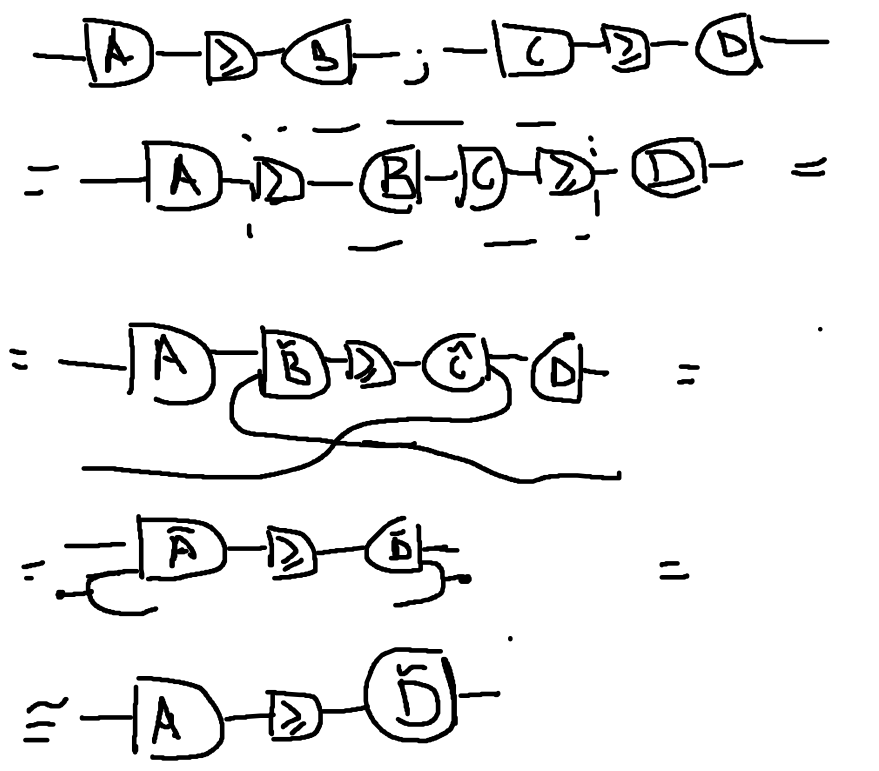
\includegraphics[width=.75\linewidth]{images//GPA/InductiveCase1NormalFormProof.png}
    \end{figure}
    And for the tensor product:
    \begin{figure}[H]
        \centering
        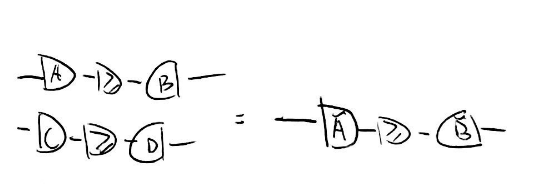
\includegraphics[width=1\linewidth]{images//GPA/InductiveCase2NormalFormProof.png}
    \end{figure}
\end{proof}

Working with a normal form defined up to isomorphism is in principle
weaker than requiring syntactic equality of terms. This choice is motivated
by the compact-closed structure, which
provides a canonical bijection $\mathrm{Hom}(A,B) \cong
\mathrm{Hom}(\mathbb{1}, A^* \otimes B)$, allowing input wires
to be treated symmetrically with output wires but only up to
this isomorphism, not up to equality. As shown in~\cite{bonchi2021polyhedral}, the same completeness
argument can be carried out using strict diagrammatic equality;
however, the derivations become significantly more involved. Since
every result established for the isomorphic normal form carries over
to the strict one, the only difference being the need to bend wires
at each step, we adopt the more convenient convention throughout.

This idea was already encountered in Section~\ref{sec:gqa},
but it is worth pausing to appreciate its significance.
The compact-closed structure does not merely allow a more convenient
notation; it enables diagrammatic reasoning to serve as a rigorous
replacement for coordinate-based algebraic manipulation while remaining
extremely intuitive: bending a wire to the left or to the right
does exactly what one would expect. Even more, a statement that would
classically require several lines of matrix algebra, tracking indices,
transposing, and substituting, can instead be verified by a sequence
of local wire manipulations, each justified by a single axiom.

This first normal form expresses every diagram as a system of inequalities
applied to a linear map. A dual normal form can be obtained by applying  the polar operator,
which we now define. The polar operator plays the  role of duality in the polyhedral setting,
exchanging the  $H$-representation (intersection of halfspaces) with the  $V$-representation
(conic hull of generators), in direct analogy with  the Farkas lemma \cite{bonchi2021.9farkas}.

\begin{definition}[Polar Operator]
    The \emph{polar operator} $-^\circ$ is the involution on generators
    defined by:
    \begin{figure}[H]
        \centering
        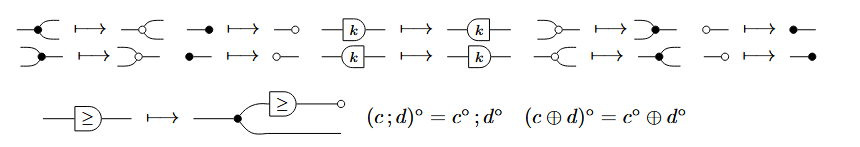
\includegraphics[width=1\linewidth]{images/GPA/PolarOperator.png}
    \end{figure}
    Its action on diagrams is defined functorially by
    $(a \circ b)^\circ = a^\circ \circ b^\circ$.
\end{definition}

\begin{proposition}[Second Normal Form]
    Every diagram $s \in \mathbf{GPA}_{\rtop}$ can be written as:
    \begin{figure}[H]
        \centering
        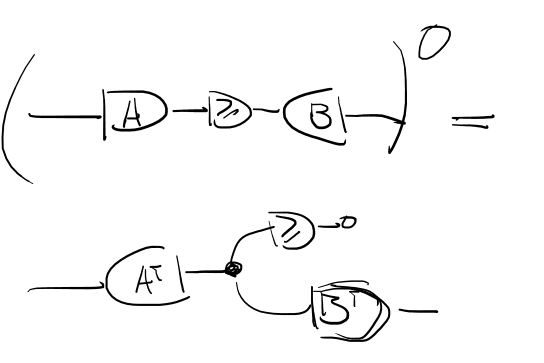
\includegraphics[width=.75\linewidth]{images//GPA/SecondNormalFormGPA.png}
    \end{figure}
\end{proposition}

\begin{proof}
    Apply the polar operator to the first normal form of every diagram
    $c \in \mathbf{GPA}_{\rtop}$. Since the polar operator is an
    involution and acts functorially, the result is again a valid diagram
    in $\mathbf{GPA}_{\rtop}$ in the claimed form.
\end{proof}

The second normal form expresses every diagram as a conic combination of
column vectors, which is precisely the $V$-representation of a polyhedral
cone. This is the representation that will drive the completeness proof:
two diagrams that are semantically equal must have the same conic hull,
and the axioms of $\mathbf{GPA}_{\rtop}$ are exactly sufficient to
witness this equality diagrammatically. We now proceed to establish the
three properties.

\begin{lemma}[Soundness]
   If $s = t$ in $\mathrm{FreeP}_{\mathbf{GPA}_{\rtop}}$, then
   $[s] = [t]$ in $\mathbf{PCRel}$.
\end{lemma}

\begin{proof}
    All axioms except those involving the newly introduced $\ge$
    generator are already present in $\mathbf{GAA}$ and therefore
    verified. It suffices to check that the new axioms preserve the
    semantics:
    \begin{figure}[H]
        \centering
        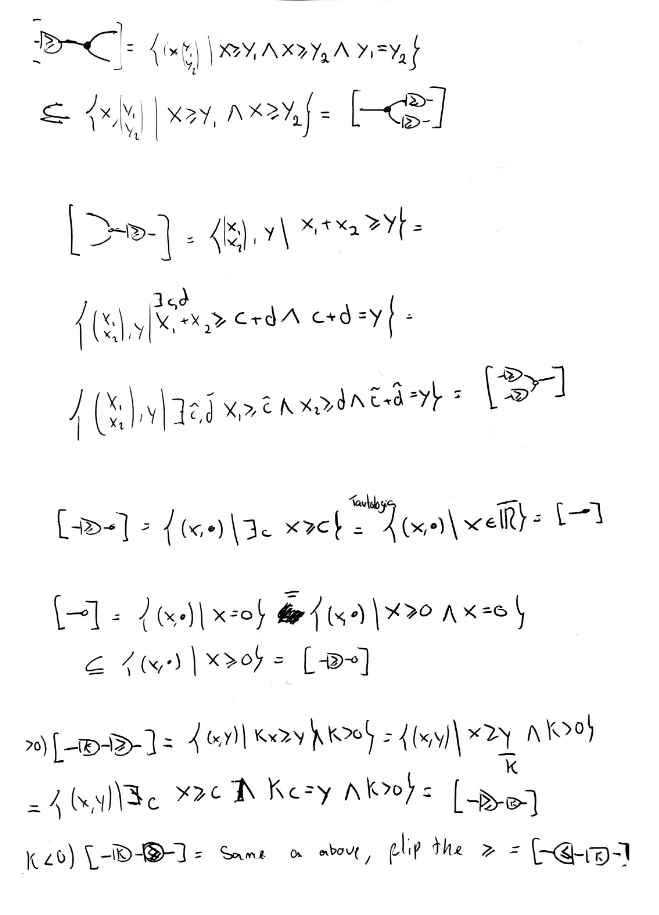
\includegraphics[width=1\linewidth]{images//GPA/SoundnessPCRel1.png}
    \end{figure}
    \begin{figure}[H]
        \centering
        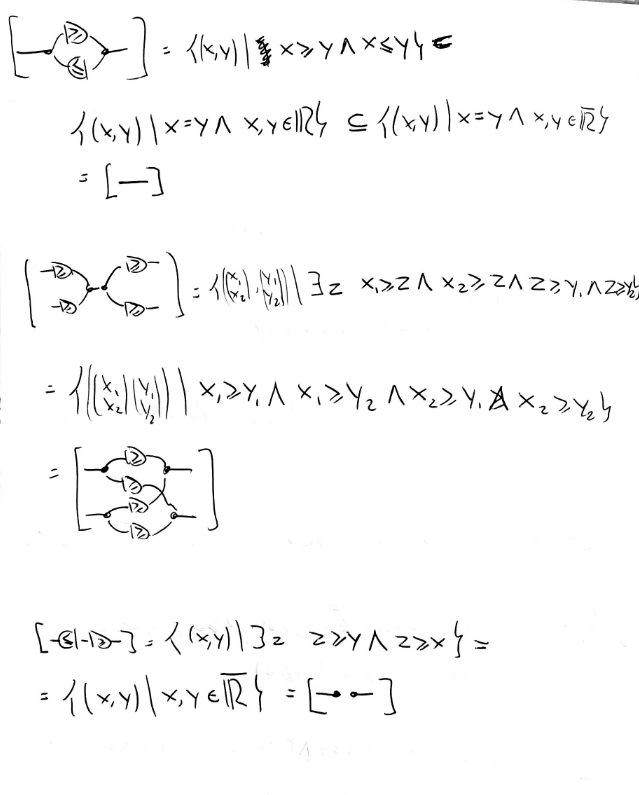
\includegraphics[width=1\linewidth]{images//GPA/SoundnessPCRel2.png}
    \end{figure}
\end{proof}

\begin{lemma}[Expressivity]
    For every $f : m \to n$ in $\mathbf{PCRel}$ there exists a
    $\Sigma$-term $s : m \to n$ in
    $\mathrm{Hom}_{\mathrm{FreeP}_{\mathbf{GPA}_{\rtop}}}(m,n)$
    such that $[s] = f$.
\end{lemma}

\begin{proof}
    By Definition~\ref{def:pcform}, every polyhedral cone has the form
    $\{x \mid Ax \ge 0,\ x \in \mathbb{R}^n\}$. This is precisely the
    interpretation of the diagram:
    \begin{figure}[H]
        \centering
        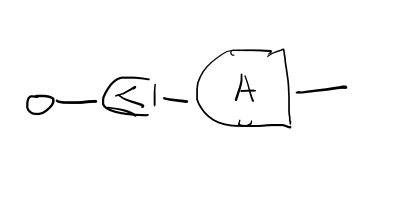
\includegraphics[width=.75\linewidth]{images//GPA/PCRelExpressivity.png}
    \end{figure}
\end{proof}

\begin{lemma}[Completeness]
   If $[s] = [t]$ in $\mathbf{PCRel}$, then $s = t$ in
   $\mathrm{FreeP}_{\mathbf{GPA}_{\rtop}}$.
\end{lemma}

\begin{proof}
    By the second normal form, we write $s$ and $t$ in
    $V$-representation form:
    \begin{figure}[H]
        \centering
        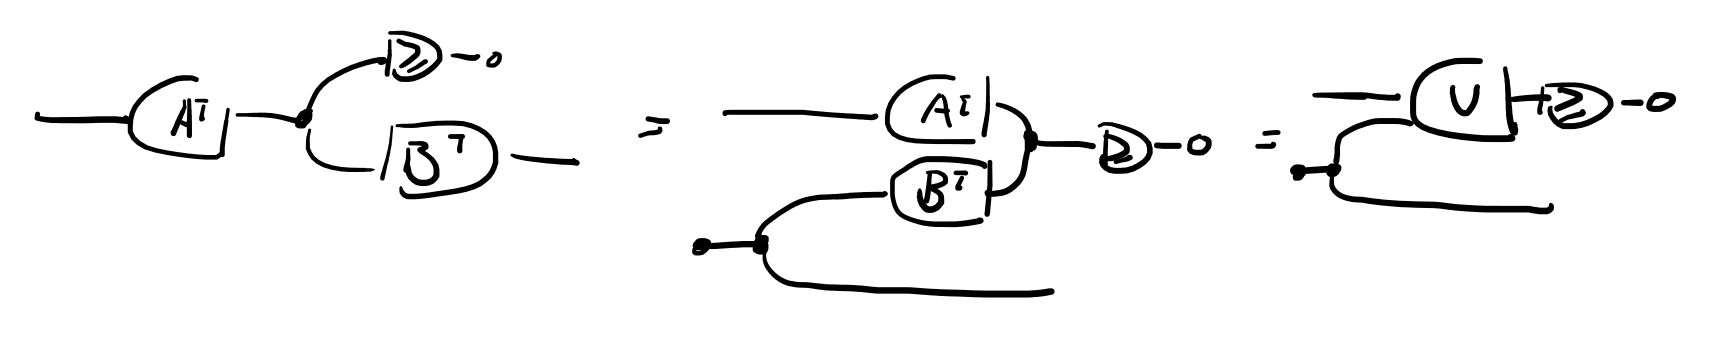
\includegraphics[width=1\linewidth]{images//GPA/ProofCompleteness1.png}
    \end{figure}
    The semantics of such a diagram is the conic hull of the column
    vectors of $V$. Since $[s] = [t]$ implies in particular
    $[s] \subseteq [t]$, the conic combinations of $V_t$ are a subset
    of those of $V_s$. Hence there exists a non-negative matrix $C$ such
    that $CV_t = V_s$. The diagrammatic witness is:
    \begin{figure}[H]
        \centering
        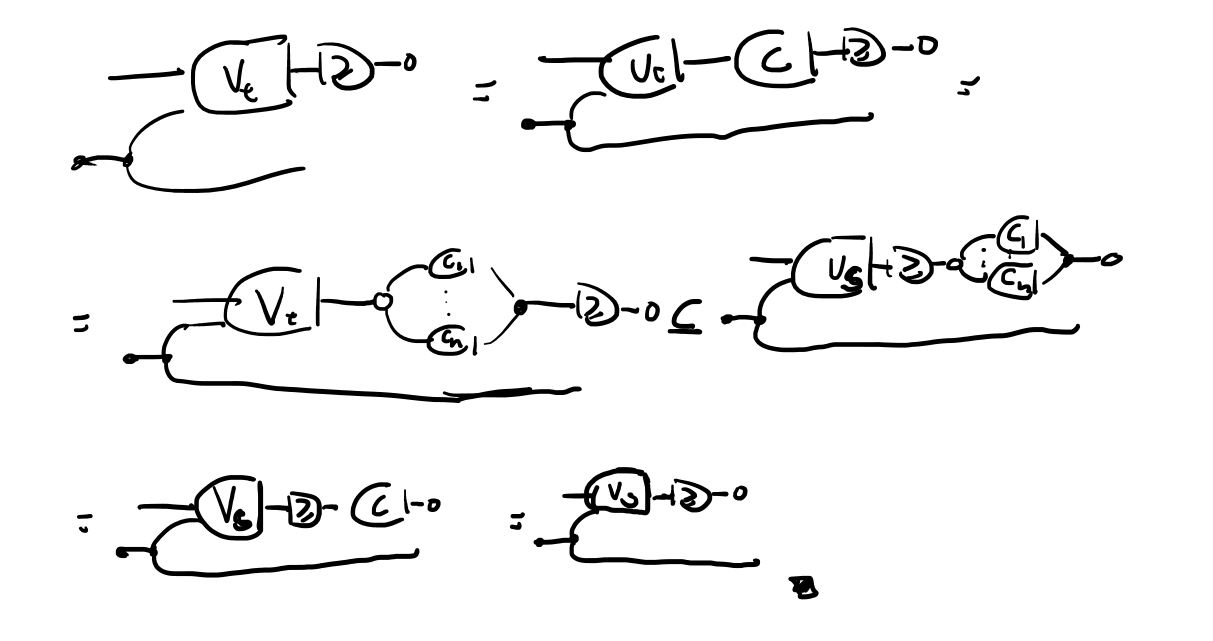
\includegraphics[width=1\linewidth]{images//GPA/ProofCompleteness2.png}
    \end{figure}
    The inclusion $[s] \subseteq [t]$ follows by the same argument,
    yielding equality.
\end{proof}

\begin{theorem}
    $\mathbf{PCRel}$ is presented by $\mathrm{FreeP}_{\mathbf{GPA}_{\rtop}}$.
\end{theorem}

\begin{proof}
    Soundness, expressivity, and completeness were established by the
    preceding three lemmas. Together they imply that the canonical PROP
    morphism is an isomorphism.
\end{proof}

\subsection{The algebra \texorpdfstring{$\mathbf{GPA}$}{GPA} and
\texorpdfstring{$\mathbf{PolyRel}$}{PolyRel}}

We now extend the theory from polyhedral cones to general polyhedra by
reintroducing the affine generator $\rtop$. Geometrically, this
corresponds to allowing translations: a polyhedron is a translated
polyhedral cone, and the generator $\rtop$ provides the syntactic means
to encode the right-hand side vector $b$ in $Ax \ge b$. The normal form,
soundness, and expressivity arguments all extend smoothly from the
homogeneous case.

\begin{theorem}[Normal Form]\label{thm:normalformgpa}
For every diagram $c$ in $\mathbf{GPA}$, there exists a diagram $d$
such that $c = d$ modulo the axioms and $d$ is of the form:
    \begin{figure}[H]
        \centering
        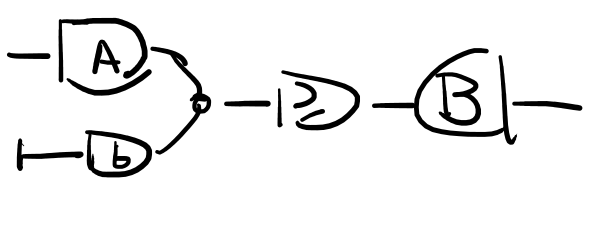
\includegraphics[width=1\linewidth]{images/GPA/NormalFormGPA.png}
    \end{figure}
\end{theorem}

\begin{proof}
    The derivation proceeds directly. Let $c$ be a
    diagram of \textbf{GPA}. Then we can collect all $\rtop$ on the left such
    that $c'$ is a diagram of $\textbf{GPA}_{\rtop}$

    \begin{figure}[H]
       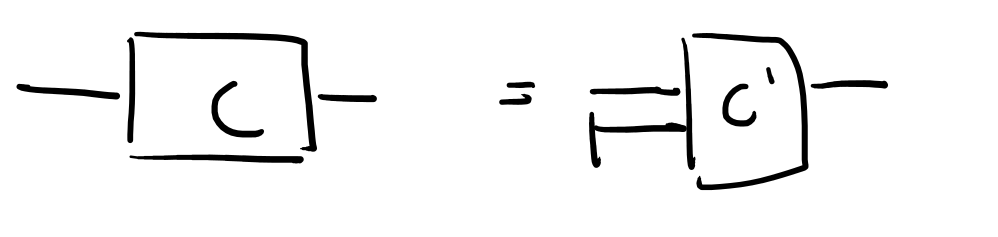
\includegraphics[width=1\linewidth]{images/GPA/affineGPAProof1.png}
    \end{figure}

    From \ref{thm:FirstNormalForm} we know that $c'$ admits a normal form in
    terms of matrices A and B. Breaking down the matrix A in columns we get:

    \begin{figure}[H]
       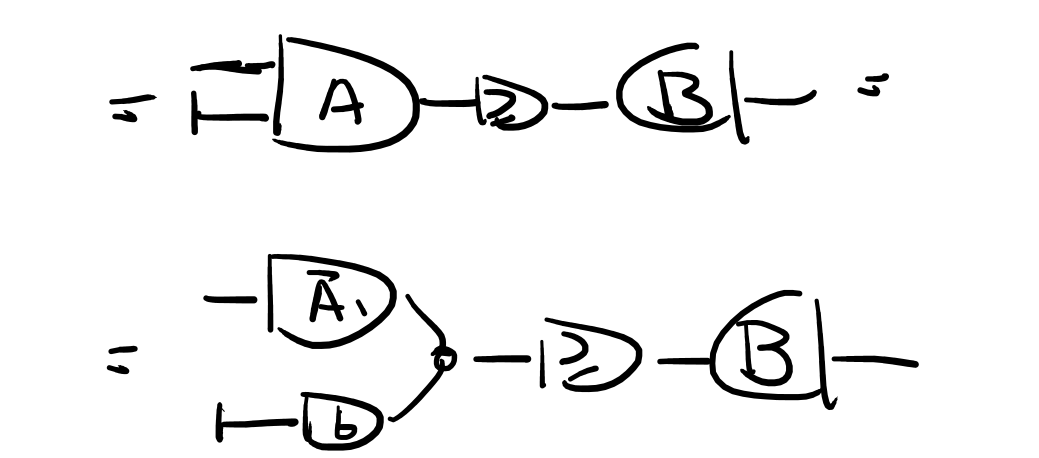
\includegraphics[width=1\linewidth]{images/GPA/affineGPAProof2.png}
    \end{figure}

    thus the thesis.
\end{proof}

\begin{lemma}[Soundness]
   If $s = t$ in $\mathrm{FreeP}_{\mathbf{GPA}}$, then $[s] = [t]$
   in $\mathbf{PolyRel}$.
\end{lemma}

\begin{proof}
    This follows immediately from the soundness of $\mathbf{PCRel}$.
    Since the generator $\rtop$ introduces no new axioms beyond those
    already verified for $\mathbf{PCRel}$ and $\mathbf{GAA}$, and both
    of those theories are sound in $\mathbf{PolyRel}$, soundness carries
    over directly.
\end{proof}

\begin{lemma}[Expressivity]
    For every $f : m \to n$ in $\mathbf{PolyRel}$ there exists a
    $\Sigma$-term $s : m \to n$ in
    $\mathrm{Hom}_{\mathrm{FreeP}_{\mathbf{GPA}}}(m,n)$
    such that $[s] = f$.
\end{lemma}

\begin{proof}
    By Definition~\ref{polyform}, every polyhedron has the form
    $\{x \mid Ax \ge b\}$. Appealing to this representation directly,
    the polyhedron is expressed as the interpretation of the following
    diagram, where the generator $\rtop$ encodes the right-hand side
    vector $b$:
    \begin{figure}[H]
        \centering
        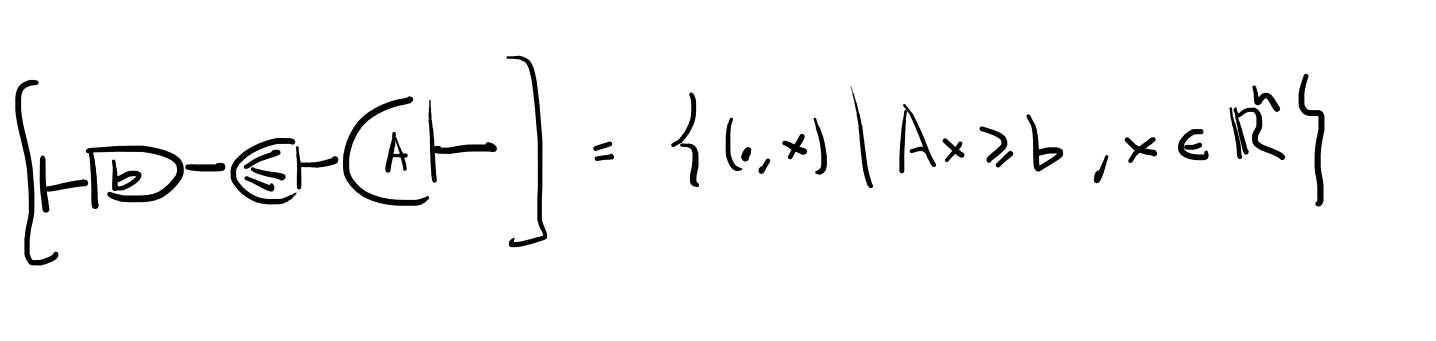
\includegraphics[width=1\linewidth]{images/GPA/ExpressivityPolyRel.png}
    \end{figure}
\end{proof}

\begin{lemma}[Completeness]
    If $[s] = [t]$ in $\mathbf{PolyRel}$, then $s = t$ in
    $\mathrm{FreeP}_{\mathbf{GPA}}$.
\end{lemma}

\begin{proof}
    Every polyhedron $P$ can be homogenised by introducing a slack variable,
    reducing the affine case to the conic one
    $P^H = \{(x,y) \in k^{n+1} | Ax + by \ge 0, y \ge 0\}$ which
    admits a normal form \ref{thm:FirstNormalForm}.
    Under this homogenisation, for each two diagrams $s, t \in \mathbf{GPA}$
    with $[s] = [t]$ in  $\mathbf{PolyRel}$, there are $s', t'$
    in $\mathbf{GPA}_{\rtop}$ such that $[s'] = [s]^H, [t'] = [t]^H $.
    Since two polyhedrals $P,Q$ are equal iff $P^H = Q^H$, then $s$ and
    $t$ have equal semantics in $\mathbf{PCRel}$.
    Completeness of $\mathbf{GPA}_{\rtop}$ then gives equality
    of the  homogenised diagrams, and de-homogenising recovers
    equality of $s$  and $t$ in $\mathrm{FreeP}_{\mathbf{GPA}}$.

    Diagrammatically this goes as follows:
    \begin{figure}[H]
        \centering
        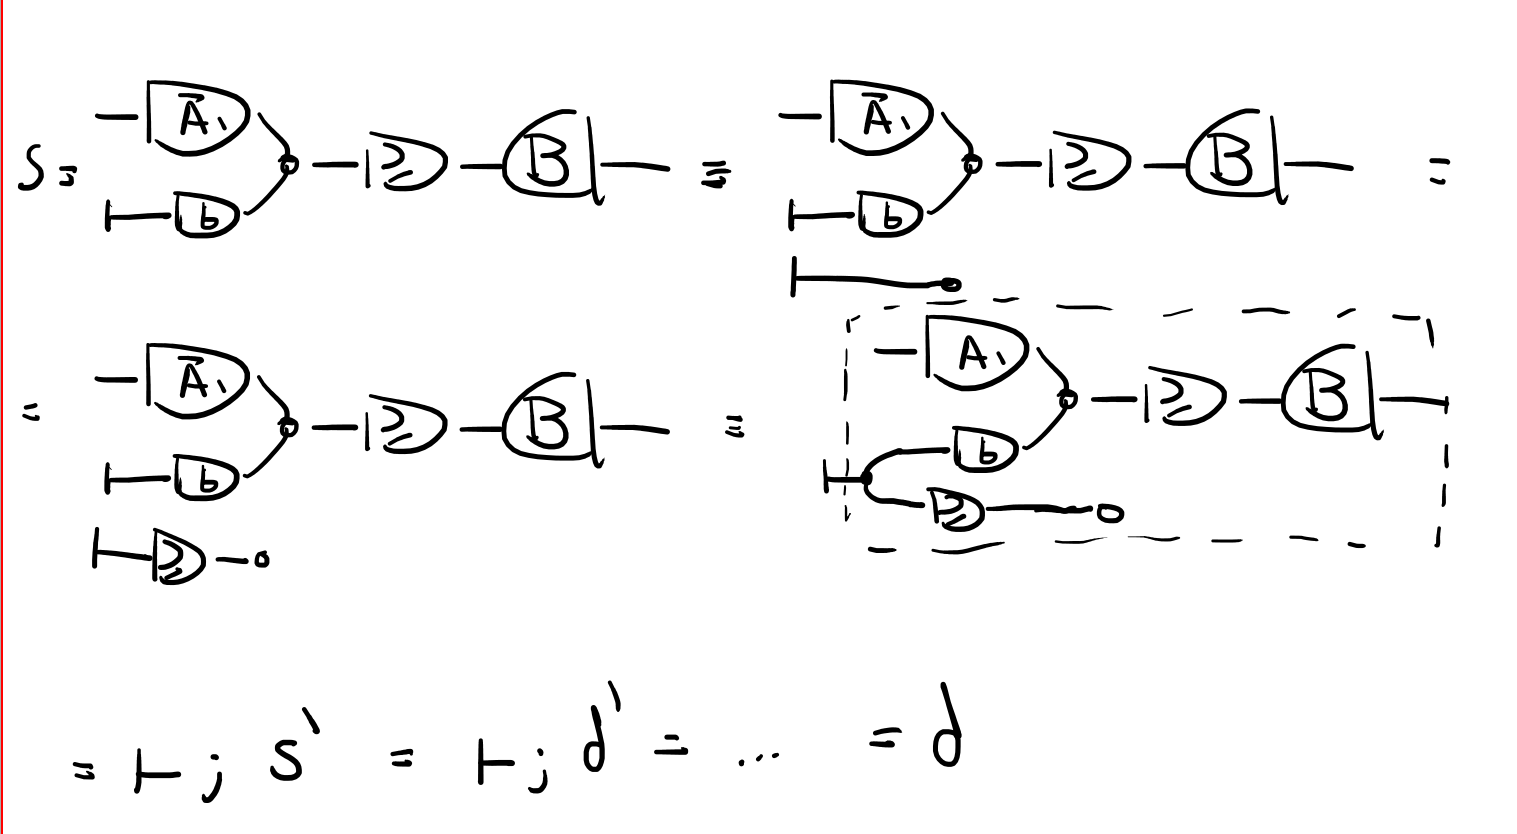
\includegraphics[width=1\linewidth]{images/GPA/CompletenessGPAProof.png}
    \end{figure}

    Whereas the interpretation of the diagram in the dotted box is
    $\{(x,y,z) \in k^m | Ax + by \ge Bz, y \ge 0\}$, which is the same
    as $P^H$. Therefore, the semantics of $s'$ is that of the homogenisation
    of $[s]$ and follows the above argument.
\end{proof}

\begin{theorem}
    $\mathbf{PolyRel}$ is presented by $\mathrm{FreeP}_{\mathbf{GPA}}$.
\end{theorem}

\begin{proof}
    By the preceding three lemmas.
\end{proof}

\section{The Linear Programming Category}\label{sec:glp}

The two graphical theories developed so far have  each extended the categorical framework
by adding a new class of  morphisms. We now introduce the
final and most expressive theory of the thesis:
a  graphical algebra for parametric linear programs.
Linear programs combine  both the inequality structure of polyhedra and the notion of an objective function,
and their value functions are precisely the polyhedral convex  functions.
The central result of this section is the presentation of a
complete monoidal theory for right-hand side parametric linear programming.

\subsection{Preliminary Results in Linear Programming}

We begin with several classical results that establish the tight
relationship between piecewise affine convex functions, polyhedral
functions, and parametric linear programs. These will serve as the
semantic foundation for the graphical algebra introduced in the following
subsection.

\begin{definition}[Piecewise Affine Convex Function]
A function $f : \mathbb{R}^n \to \mathbb{R}$ is called
\emph{piecewise affine convex} if there exist finitely many affine
functions $a_i^\top x + b_i$, $i = 1,\dots,k$, such that
\[
f(x) = \max_{i=1,\dots,k} \{ a_i^\top x + b_i \}.
\]
\end{definition}

\begin{definition}[Polyhedral Function]
A function $f : \mathbb{R}^n \to \mathbb{R} \cup \{+\infty\}$ is
\emph{polyhedral} if its epigraph
\[
\mathrm{epi}(f) := \{ (x,t) \mid t \ge f(x) \}
\]
is a polyhedron.
\end{definition}

\begin{definition}[RHS Parametric Linear Program]
A \emph{right-hand side parametric linear program} has value function
\[
v(b) := \inf_{x} \{ c^\top x \mid Ax \ge b \}.
\]
\end{definition}

The following two propositions establish that all three notions above
are equivalent descriptions of the same class of functions. This
equivalence is the semantic cornerstone of the section: it is what
allows us to treat polyhedral functions and parametric linear programs
as morphisms in the same category.

\begin{proposition}
A function is piecewise affine convex if and only if it is a polyhedral
function.
\end{proposition}

\begin{proof}
\textbf{($\Rightarrow$)} Let
$f(x) = \max_{i=1,\dots,k} (a_i^\top x + b_i)$.
Then
\[
\mathrm{epi}(f) = \bigcap_{i=1}^k \{ (x,t) \mid t \ge a_i^\top x + b_i \},
\]
which is an intersection of finitely many halfspaces, hence a polyhedron.

\medskip
\textbf{($\Leftarrow$)} If $f$ is polyhedral, its epigraph is a
polyhedron, so there exist finitely many affine inequalities
$t \ge a_i^\top x + b_i$ such that
$f(x) = \max_{i=1,\dots,k} (a_i^\top x + b_i)$.
Thus $f$ is piecewise affine and convex.
\end{proof}

\begin{proposition}
A function $v : \mathbb{R}^m \to \mathbb{R} \cup \{+\infty\}$ is
piecewise affine convex if and only if it is the value function of a
right-hand side parametric linear program.
\end{proposition}

\begin{proof}
\textbf{($\Rightarrow$)} Let
$v(b) = \max_{i=1,\dots,k} (y^i)^\top b$
and define $Y := \mathrm{conv}\{y^1,\dots,y^k\}$.
Then $v(b) = \max_{y \in Y} b^\top y$.
Since $Y$ is a polyhedron admitting the representation
$Y = \{ y \mid A^\top y = c,\; y \ge 0 \}$,
linear programming duality gives
$v(b) = \inf \{ c^\top x \mid Ax \ge b \}$.

\medskip
\textbf{($\Leftarrow$)} Let
$v(b) = \inf \{ c^\top x \mid Ax \ge b \}$.
Dualising,
$v(b) = \sup \{ b^\top y \mid A^\top y = c,\; y \ge 0 \}$.
Since the feasible set $Y = \{ y \mid A^\top y = c,\; y \ge 0 \}$
is a polyhedron, the supremum is attained at its extreme points
$y^1,\dots,y^k$, yielding
$v(b) = \max_{i=1,\dots,k} (y^i)^\top b$.
Thus $v$ is piecewise affine convex.
\end{proof}

The following proposition is the key technical lemma for the completeness
proof of $\mathbf{GLP}$. It states that two parametric linear programs
with the same value function must share the same epigraph polyhedron,
providing the bridge between semantic equality and polyhedral equality
that the completeness argument requires.

\begin{proposition}\label{prop:equalepi}
Let
\[
v_i(y) := \inf\{\mathbf{1}^\top x \mid A_i x \ge B_i y\},
\qquad i=1,2,
\]
where $A_i \in \mathbb{R}^{m_i \times n_i}$ and
$B_i \in \mathbb{R}^{m_i \times k}$. If $v_1(y) = v_2(y)$ for all
$y \in \mathbb{R}^k$, then both programs admit a common representation
through the same epigraph polyhedron:
\[
v_i(y) = \inf\{t \mid (y,t) \in E\},
\qquad
E := \mathrm{epi}(v_1) = \mathrm{epi}(v_2).
\]
\end{proposition}

\begin{proof}
For each $i = 1,2$, the epigraph of $v_i$ satisfies
\[
(y,t) \in \mathrm{epi}(v_i)
\iff
\exists x : A_i x \ge B_i y,\ \mathbf{1}^\top x \le t,
\]
so $\mathrm{epi}(v_i)$ is the projection onto $(y,t)$ of the polyhedron
$P_i = \{(x,y,t) \mid A_i x \ge B_i y,\ \mathbf{1}^\top x \le t\}$.
Projections of polyhedra are polyhedra, so each $\mathrm{epi}(v_i)$ is
a polyhedron. Since $v_1 = v_2$ pointwise, we have
$\mathrm{epi}(v_1) = \mathrm{epi}(v_2) =: E$.
Setting $E = \{(y,t) \mid Cy + dt \ge 0\}$, we obtain
$v_i(y) = \inf\{t \mid Cy + dt \ge 0\}$ for both $i = 1, 2$.
\end{proof}

\subsection{Graphical Algebra for Parametric Linear Programs}

With the semantic equivalences established, we now introduce the final
graphical algebra of the thesis. The algebra $\mathbf{GLP}$ extends
$\mathbf{GPA}$ with a single new generator whose semantics encodes the
linear objective function $c^\top x$. Just as the gray arrow in
$\mathbf{GQA}$ lifted the theory from binary relations to weighted
relations by "measuring" the $\ell_2$ norm, this new generator lifts $\mathbf{GPA}$
from polyhedral constraints to full linear programs by attaching a
linear cost to the feasible region.

\begin{definition}[$\mathbf{GLP}$]
    We call $\mathbf{GLP}$ the symmetric monoidal theory obtained by
    extending $\mathbf{GPA}$ with the following generator:
    \begin{figure}[H]
        \centering
        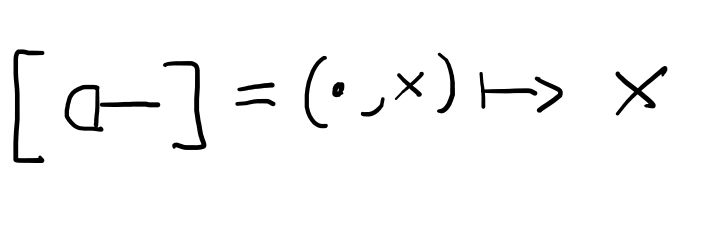
\includegraphics[width=0.75\linewidth]{images//GLP/NewGenerator.png}
    \end{figure}
    together with the following axioms governing its interaction with
    the existing generators:
    \begin{figure}[H]
        \centering
        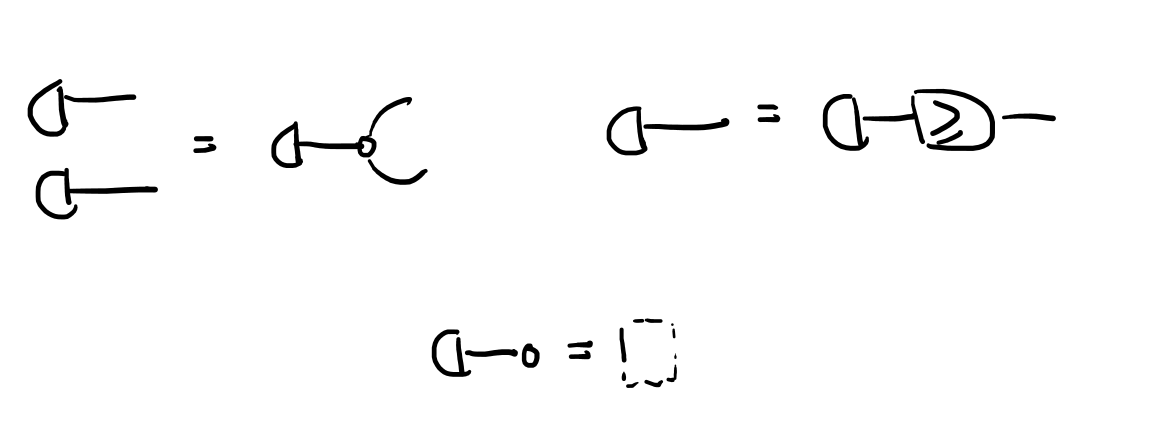
\includegraphics[width=0.75\linewidth]{images//GLP/NewAxioms.png}
    \end{figure}
\end{definition}

The axioms represent expected properties of the linear cost function.
The one on the left express the linear property $f(x) + f(y) = f(x+y)$.
Observe that $f$ is the interpretation of the $\mushroom$ and the
sum denotes the vertical composition; composing two $\mushroom$ vertically
(adding) is the same as adding the wires in a single $\mushroom$. In turn, the
equation on the left express the fundamental property of
minimization, the infimum of any quantity lies in its lower bound.
\[\inf_x \{ x | x \ge y \} =  y\]

Finally, the axiom at the middle is
the tautological case. \[inf 0 = 0\]


\begin{definition}
    We call $\mathrm{FreeP}_{\mathbf{GLP}}$ the PROP freely generated
    by $\mathbf{GLP}$.
\end{definition}

We now define the two equivalent semantic categories for this algebra.
The first, $\mathbf{LPRel}$, describes morphisms as parametric linear
programs; the second, $\mathbf{PolyFun}$, describes them as polyhedral
functions. The equivalence between the two follows immediately from the
propositions above, and we will use both descriptions interchangeably
according to which is more convenient.

\begin{definition}[The prop $\mathbf{LPRel}$ of Linear Programs]
The prop $\mathbf{LPRel}$ is defined as follows:
\begin{itemize}
    \item Objects are natural numbers $n \in \mathbb{N}$, interpreted
    as the space $\mathbb{R}^n$.
    \item A morphism $n \to m$ is a right-hand side parametric linear
    program with value function
    \[
    (x,y) \mapsto \inf_z \{ c^\top z \mid Az \ge B[x\ y]^\top \},
    \]
    where $x \in \mathbb{R}^n$ and $y \in \mathbb{R}^m$.
    \item Composition is given by minimisation over the shared variable.
    \item The monoidal product on objects is addition $n \otimes m := n+m$,
    and on morphisms is direct sum.
\end{itemize}
\end{definition}

\begin{definition}[The prop $\mathbf{PolyFun}$ of polyhedral functions]
The prop $\mathbf{PolyFun}$ is defined as follows:
\begin{itemize}
    \item Objects are natural numbers $n \in \mathbb{N}$, interpreted
    as the space $\mathbb{R}^n$.
    \item A morphism $n \to m$ is a polyhedral function
    $f : \mathbb{R}^{n+m} \to \overline{\mathbb{R}}$.
    \item Composition is given by infimal convolution over the shared
    variable.
    \item The monoidal product on objects is addition $n \otimes m := n+m$,
    and on morphisms is $f \otimes g := f + g$.
\end{itemize}
\end{definition}

\begin{remark}
    The two categories are isomorphic as PROPs: $\mathbf{PolyFun} \cong
    \mathbf{LPRel}$. This is a direct consequence of the equivalence
    between polyhedral functions and right-hand side parametric linear
    programs established in the propositions above. We will therefore
    use the two names interchangeably, choosing whichever description is
    more natural in a given context.
\end{remark}

The normal form theorem for $\mathbf{GLP}$ extends the one for
$\mathbf{GPA}$: every diagram can be reduced to a $\mathbf{GPA}$ block
encoding the constraints, composed with the new generator encoding the
objective. The proof proceeds by structural induction, using the existing
normal form for $\mathbf{GPA}$ as the inductive base.

\begin{theorem}[Normal Form]\label{thm:NormalFormGLP}
    For every diagram $c \in \mathbf{GLP}$, there exists a diagram $c'$
    in normal form such that $c = c'$:
    \begin{figure}[H]
        \centering
        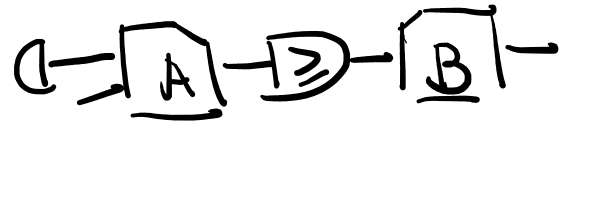
\includegraphics[width=0.75\linewidth]{images//GLP/NormalForm.png}
    \end{figure}
    With $A$ and be being an affine transformation. Namely:
    \begin{figure}[H]
        \centering
        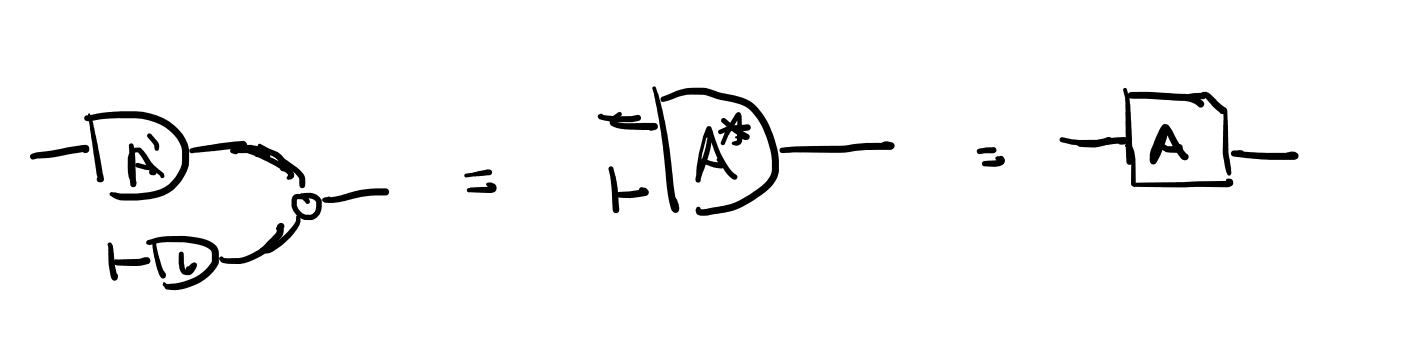
\includegraphics[width=0.75\linewidth]{images/GLP/Affine transformation.png}
    \end{figure}
\end{theorem}

\begin{proof}
    The proof is by structural induction. First we show the two base cases:
    \begin{itemize}
        \item The generator $\mushroom$
        \begin{figure}[H]
            \centering
            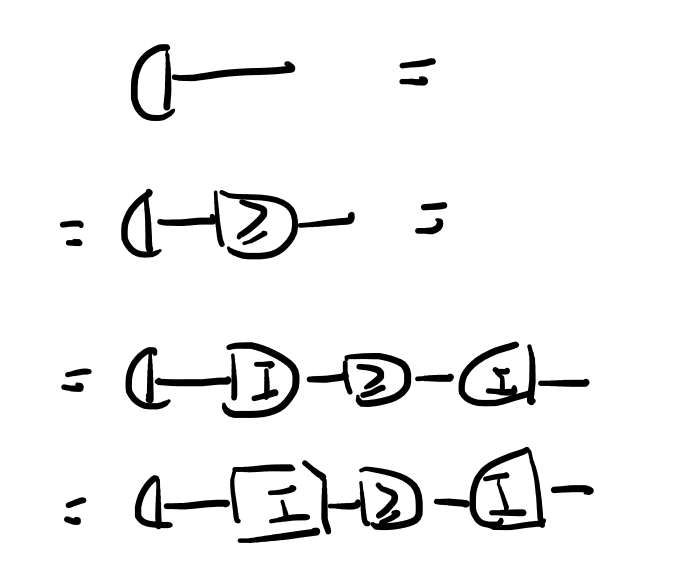
\includegraphics[width=0.75\linewidth]{images//GLP/ProofNormalFOrm1.png}
        \end{figure}
        \item A diagram c \in \textbf{GPA}

        \begin{figure}[H]
            \centering
            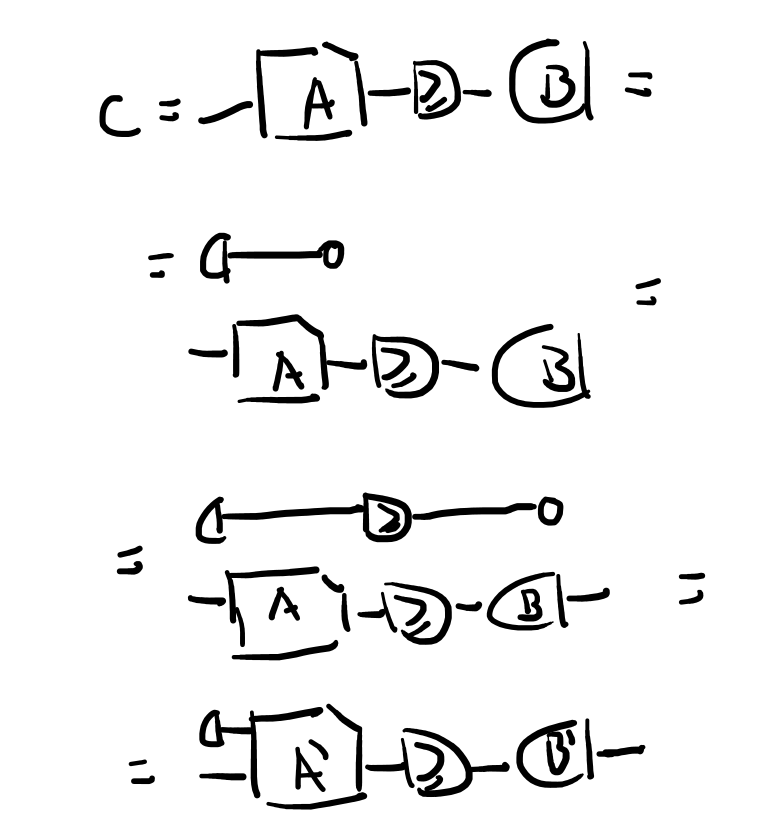
\includegraphics[width=0.75\linewidth]{images//GLP/ProofNormalForm2.png}
        \end{figure}
    \end{itemize}
    For the inductive step, we verify that for any two diagrams
    $c, d \in \mathbf{GLP}$ satisfying the inductive hypothesis,
    both horizontal and vertical composition preserve the normal form.
    Closure under vertical composition follows immediately from the normal form.
    For horizontal composition, we apply Fourier-Motzkin Elimination in the \textbf{GLP}
    part of the diagram to recover the normal form.
\end{proof}

The following corollary reveals the geometric meaning of the normal form:
the $\mathbf{GPA}$ part of every $\mathbf{GLP}$ diagram encodes the
epigraph of the corresponding value function. This is the key structural
insight connecting the syntax to the semantic equivalence of
Proposition~\ref{prop:equalepi}.

\begin{corollary}[Epigraph Form]\label{cor:epigraph form}
    Given a diagram $d \in \mathbf{GLP}$ in normal form, it can always
    be rewritten as a diagram $d'$ of the form:
    \begin{figure}[H]
        \centering
        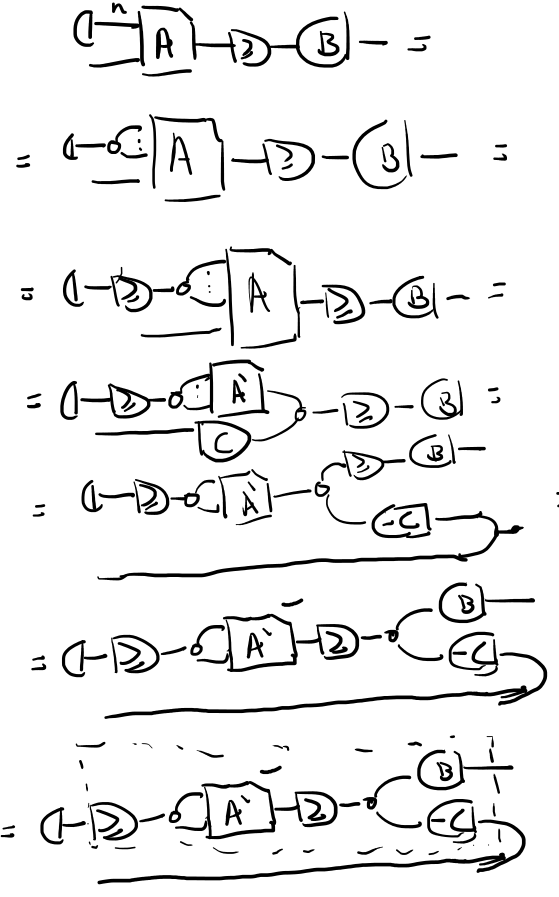
\includegraphics[width=1\linewidth]{images//GLP/epiForm1.png}
    \end{figure}
    where the semantics of the dotted diagram is
    \[\left\{(t,y)\mid \exists\, x,\; A'x + a \ge [B\; -C]\, y,\; t\ge x,\; y =
    \begin{bmatrix} y_1 \\ y_2 \end{bmatrix}\right\}\].
    This is the epigraph of the original diagram $d$
    \begin{align*}
        [d](y_1, y_2) &= \inf_{z} \; z \quad \text{s.t. } A z + a \ge B y_1 - C y_2 \\
        \mathrm{epi}([d]) &= \left\{(t, y_1, y_2) \mid \exists\, z \le t,\;
            A z + a \ge B y_1 - C y_2 \right\}
    \end{align*}
    such that $A = [A' \;C]$. We call this the \emph{epigraph form} of a linear program.
\end{corollary}

We are now ready to prove the three presentation properties for
$\mathbf{GLP}$.

\begin{lemma}[Expressivity]
    For every $f : m \to n$ in $\mathbf{PolyFun}$ there exists a
    $\Sigma$-term $s : m \to n$ in
    $\mathrm{Hom}_{\mathrm{FreeP}_{\mathbf{GLP}}}(m,n)$
    such that $[s] = f$.
\end{lemma}

\begin{proof}
    Since every polyhedral function is the maximum of a finite family of
    affine functions, it suffices to show that every piecewise affine
    convex function is expressible in $\mathbf{GLP}$. For an arbitrary
    such function $f(y) = \max_i R_i(y)$, where $\{R_i\}_{i=1,\dots,n}$
    is a family of affine functions, the following diagram provides the
    required syntactic representative:
    \begin{figure}[H]
        \centering
        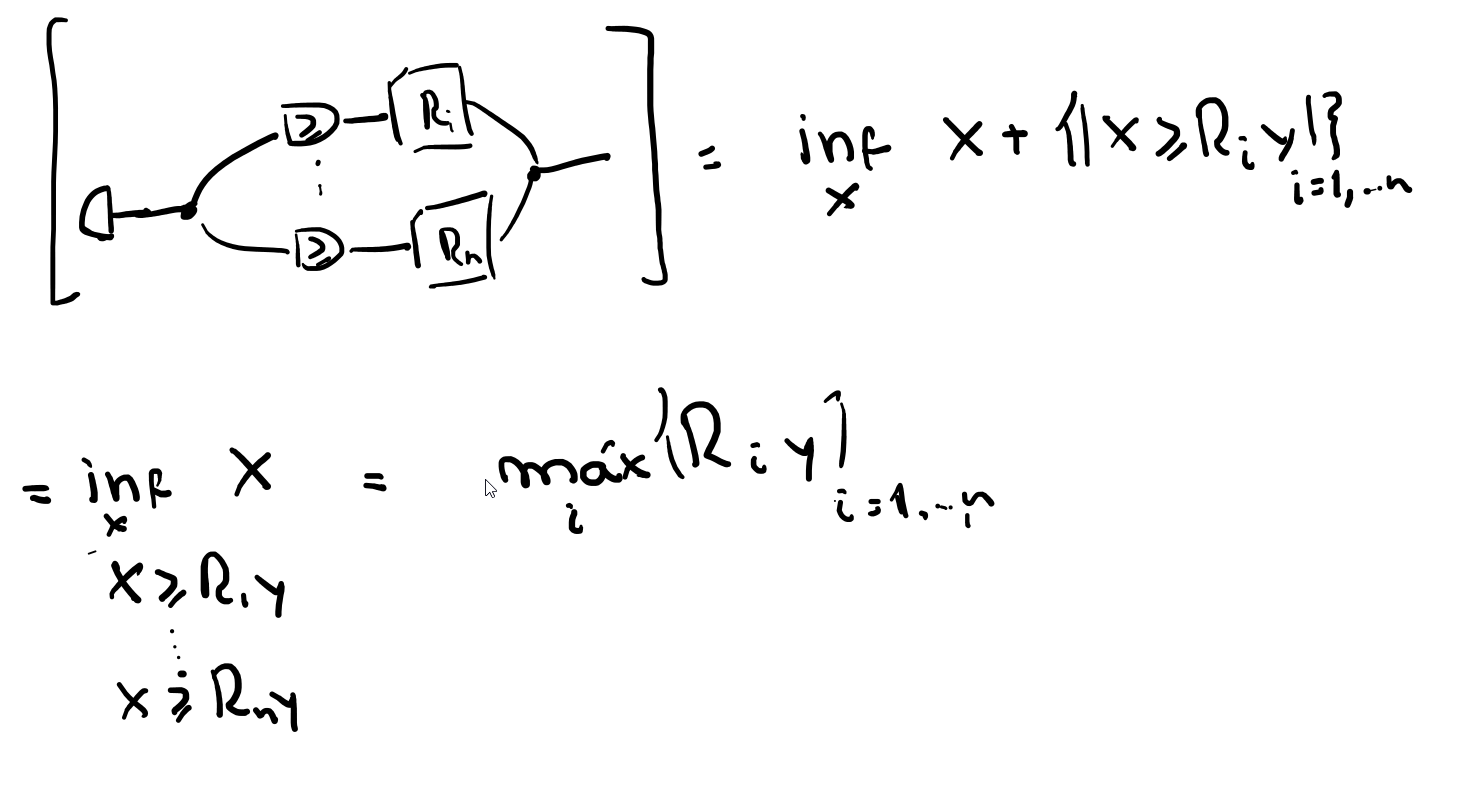
\includegraphics[width=0.75\linewidth]{images//GLP/ExpressivityGLP.png}
    \end{figure}
\end{proof}

\begin{lemma}[Soundness]
   If $s = t$ in $\mathrm{FreeP}_{\mathbf{GLP}}$, then $[s] = [t]$
   in $\mathbf{PolyFun}$.
\end{lemma}

\begin{proof}
    All axioms inherited from $\mathbf{GPA}$ are already sound by the
    results of the previous section. It suffices to verify that the new
    axioms involving the LP generator preserve the semantics, which
    follows by direct computation:
    \begin{figure}[H]
        \centering
        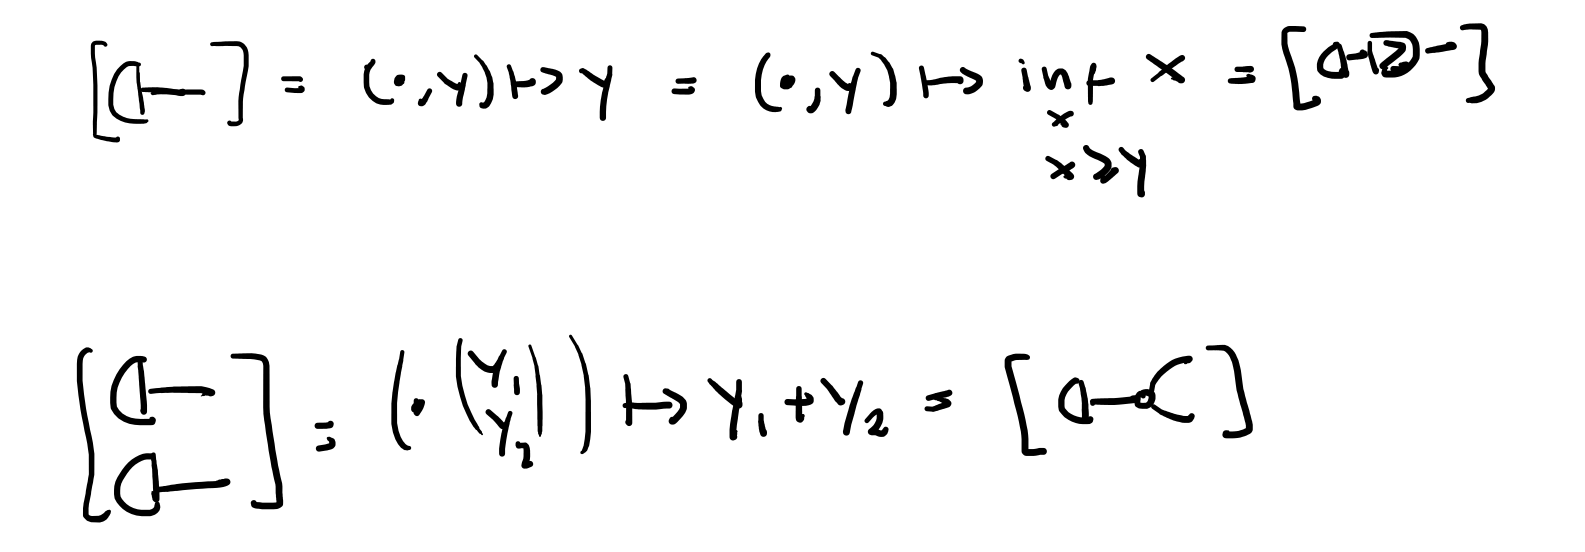
\includegraphics[width=0.75\linewidth]{images//GLP/Soundness.png}
    \end{figure}
\end{proof}

The final result of the thesis is the completeness theorem for
$\mathbf{GLP}$. The proof brings together all the main tools developed
throughout: the epigraph form of Corollary~\ref{cor:epigraph form}, the
shared epigraph property of Proposition~\ref{prop:equalepi}, the
completeness of $\mathbf{GPA}$, and the FME-based normal form. We state
it as a conjecture because the completeness of the $\mathbf{GPA}$
polyhedra case, which the argument appeals to, still has a gap in the
proof of Completeness for $\mathbf{PolyRel}$; subject to that result,
the argument below goes through.

\begin{lemma}[Completeness]
   If $[c] = [d]$ in $\mathbf{PolyFun}$, then $c = d$ in
   $\mathrm{FreeP}_{\mathbf{GLP}}$.
\end{lemma}

\begin{proof}
    Let $v_1 = [c]$ and $v_2 = [d]$. By assumption $v_1 = v_2$, so
    Proposition~\ref{prop:equalepi} gives
    $\mathrm{epi}(v_1) = \mathrm{epi}(v_2) =: E$.

    By Corollary~\ref{cor:epigraph form}, both $c$ and $d$ admit
    epigraph forms $c = \mushroom ; c^*$ and $d = \mushroom ; d^*$
    with $[c^*] = [d^*] = E$ in $\mathbf{PolyRel}$:
    \begin{figure}[H]
        \centering
        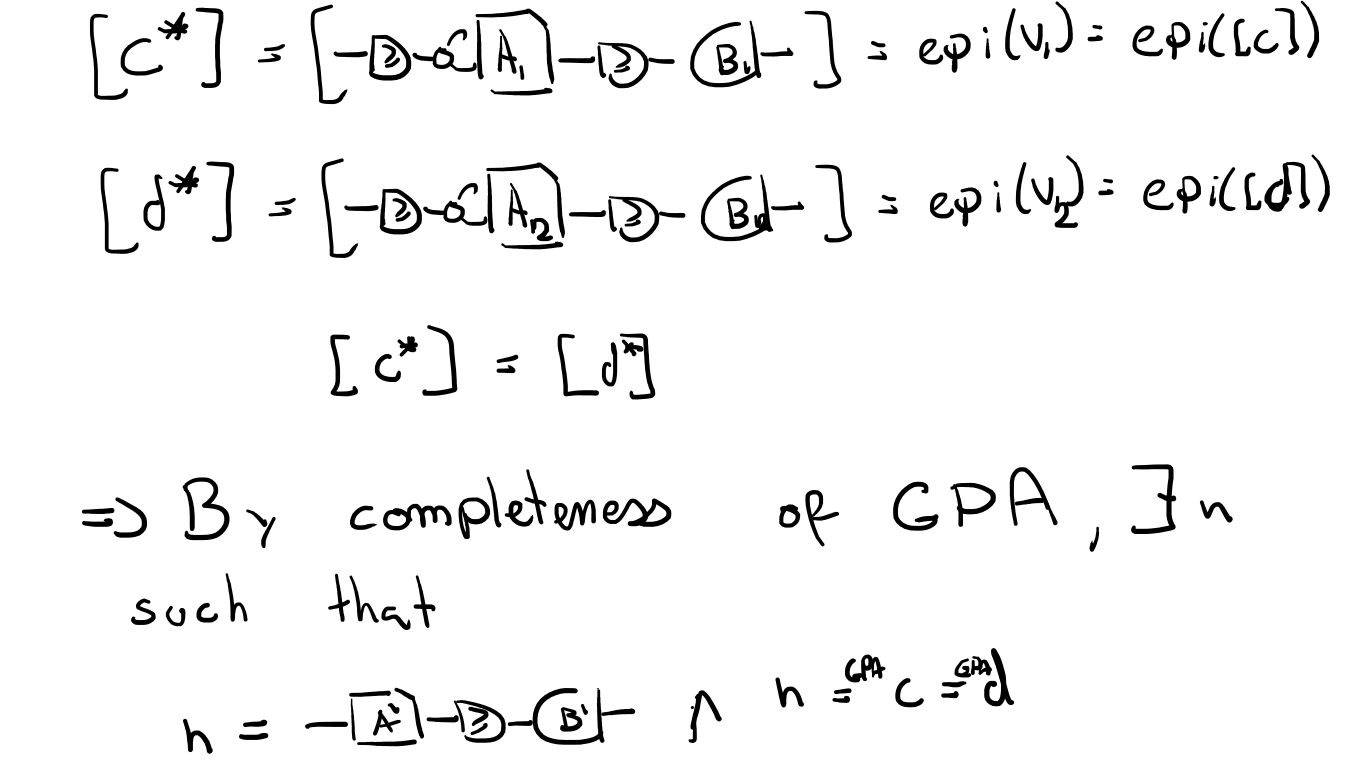
\includegraphics[width=0.75\linewidth]{images//GLP/proofCompleteness1.png}
    \end{figure}
    Since $[c^*] = [d^*]$ in $\mathbf{PolyRel}$, completeness of
    $\mathbf{GPA}$ gives $c^* = d^* = n$ in
    $\mathrm{FreeP}_{\mathbf{GPA}}$:
    Therefore,
    \[
    c = \mushroom ; c^* = \mushroom ; n = \mushroom ; d^* = d,
    \]
    as witnessed diagrammatically by:
    \begin{figure}[H]
        \centering
        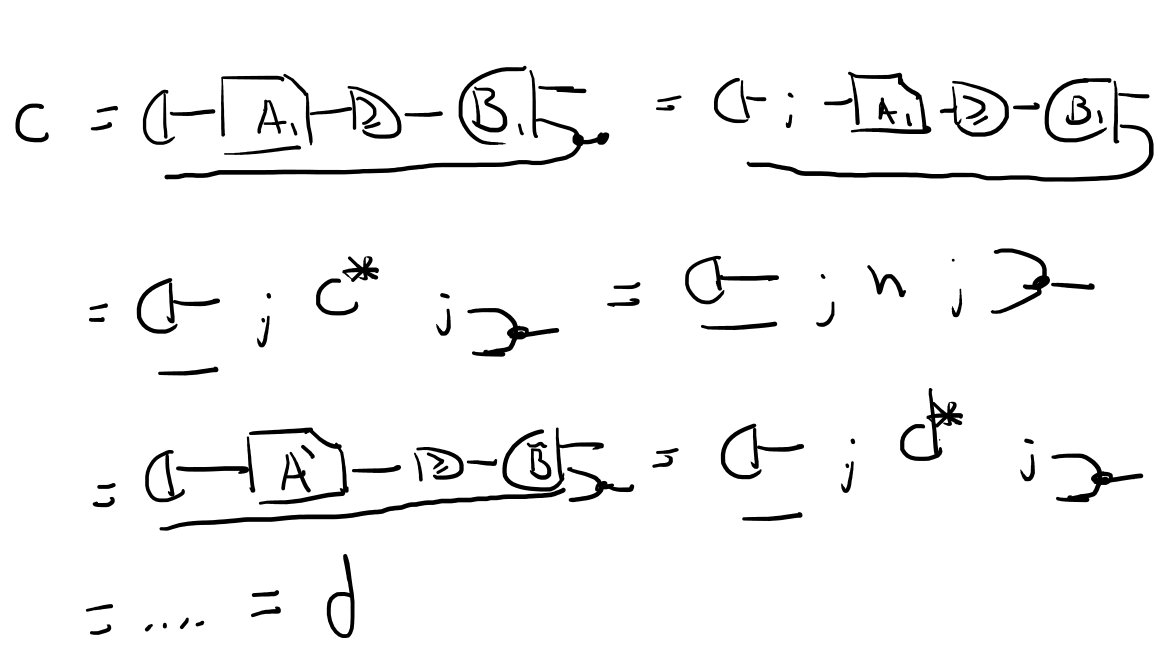
\includegraphics[width=0.75\linewidth]{images//GLP/proofCompleteness4.png}
    \end{figure}
\end{proof}

As consequence of the three lemmas above

\begin{theorem}
    $\mathbf{LPRel}$ and $\mathbf{PolyFun}$ are both presented by $\mathrm{FreeP}_{\mathbf{GLP}}$.
\end{theorem}
\begin{proof}
    By the preceding three lemmas.
\end{proof}

Finally, we've built, through the addition of one generator and three axioms,
an elegant and complete diagrammatical theory for Parametric Linear Programming.
We argue that, such result, not just unlocks a new way to interact with LP problems in a algebraic
and computational way, but also provide a new perspective to optimization through the lens of
a compositional framework. Whereas optimization, namely LP problems, are lifted above
the settings of functional thinking and achieves a new status as a relational-theoretic
field embeded into the Extended-Lawvere Quantale category.

The \textbf{GLP} theory, in turn, has a natural extension to a even more expressive theory
when enriched with the gray arrow generator from \textbf{GQA}. We believe that the class
of quadratic programs could be, just as was done in this work, fully axiomatized by such
broader SMIT. However, such studies are left for future works, along with other possible applications
of current results.

\section{Conclusion}

This thesis begun with a philosophical claim, that the nature
of a mathematical object is fully determined by its relationships to other objects,
and that universal constructions reveal connections invisible to any particular
viewpoint. Optimization, by contrast, is often presented as a
collection of problem-specific techniques. The central claim of the thesis is
that these two perspectives are not merely compatible, but that optimization
\emph{emerges} from categorical structure naturally, as an intrinsic property of
relational composition and is natural to mathematical thinking.

To demonstrate that, we took advantage of the expressivity of graphical languages.
The development followed a strict linear discipline, adding exactly one new
generator at a time and verifying at each step that the resulting algebra is
sound, expressive, and complete with respect to a precisely defined semantic
category. This methodology is itself one
of the work's implicit arguments. The fact that such a linear development is
possible, that each new class of optimization problems requires only a single
additional generator and a finite set of axioms, is evidence that the
compositional structure is not imposed artificially but is genuinely present in
the mathematics.

The following diagram illustrates the relationships among all the categorical
structures developed in this thesis. Moving upward corresponds to increasing
expressive power: each layer generalises the one below by enlarging the class
of morphisms, while preserving the compositional structure. The morphisms
marked $\hookrightarrow$ are inclusion functors, embedding each category as a
full subcategory of the one above. The morphism marked $\mathbf{1}$ denotes the
indicator function embedding, which sends a set-valued relation to its
$\{0,+\infty\}$-valued characteristic function.

What this hierarchy makes visible is something that would be difficult to
articulate within any single one of its layers. Polyhedral relations and
quadratic relations are not merely two classes of optimization problems that
happen to admit graphical representations; they are parallel enrichments of the
same underlying affine structure, each adding a different kind of expressive
power. Their common base in \textbf{AffRel} and their common embedding into
\textbf{Cost-Relations} is not an accident of notation but a theorem, witnessed
by the inclusion functors in the diagram. A single compositional
framework within which relations, functions, constraints, and objectives are
unified as morphisms, and within which optimization is not a technique applied
to a problem but an algebraic operation itself.

The broader significance of this perspective lies in what it enables beyond
the specific algebras treated here. The diagrammatic calculus established for
\textbf{GLP} plays the same role for linear programming that Graphical Linear
Algebra plays for matrices: it provides a language of normal forms, rewriting
rules, and completeness theorems within which optimization arguments can be
carried out symbolically, before and independently of any numerical computation.
This opens several directions for future work. One of them is the exploration of the functoriality of
the bifunction adjoint established in Section~3. Such observation suggests that a duality theory
analogous to LP duality should be expressible diagrammatically in these settings
as well.

A more applied direction concerns the computational implications of diagrammatic
normal forms. If two optimization problems are equal as morphisms in
\textbf{LPRel} if and only if their diagrams are related by the rewriting rules
of \textbf{GLP}, then diagram simplification is problem simplification: a
rewriting system on string diagrams is simultaneously a symbolic preprocessor
for optimization solvers. Such an application of graphical algebras for theorem
solvers was already pointed in other works \cite{bonchi2021.9farkas,bonchi2021polyhedral}.

This thesis has taken the first step of the road to fully express optimization within
it's own algebraical settings. It has shown that the language of string diagrams can absorb,
unify, and extend three of the central theories of mathematical optimization within a single
categorical framework built incrementally from the ground up. The theories here presented are
not three separate pieces wearing categorical clothing, but a single theory, viewed at three
different levels of expressive resolution.

\begin{figure}[H]
    \centering
    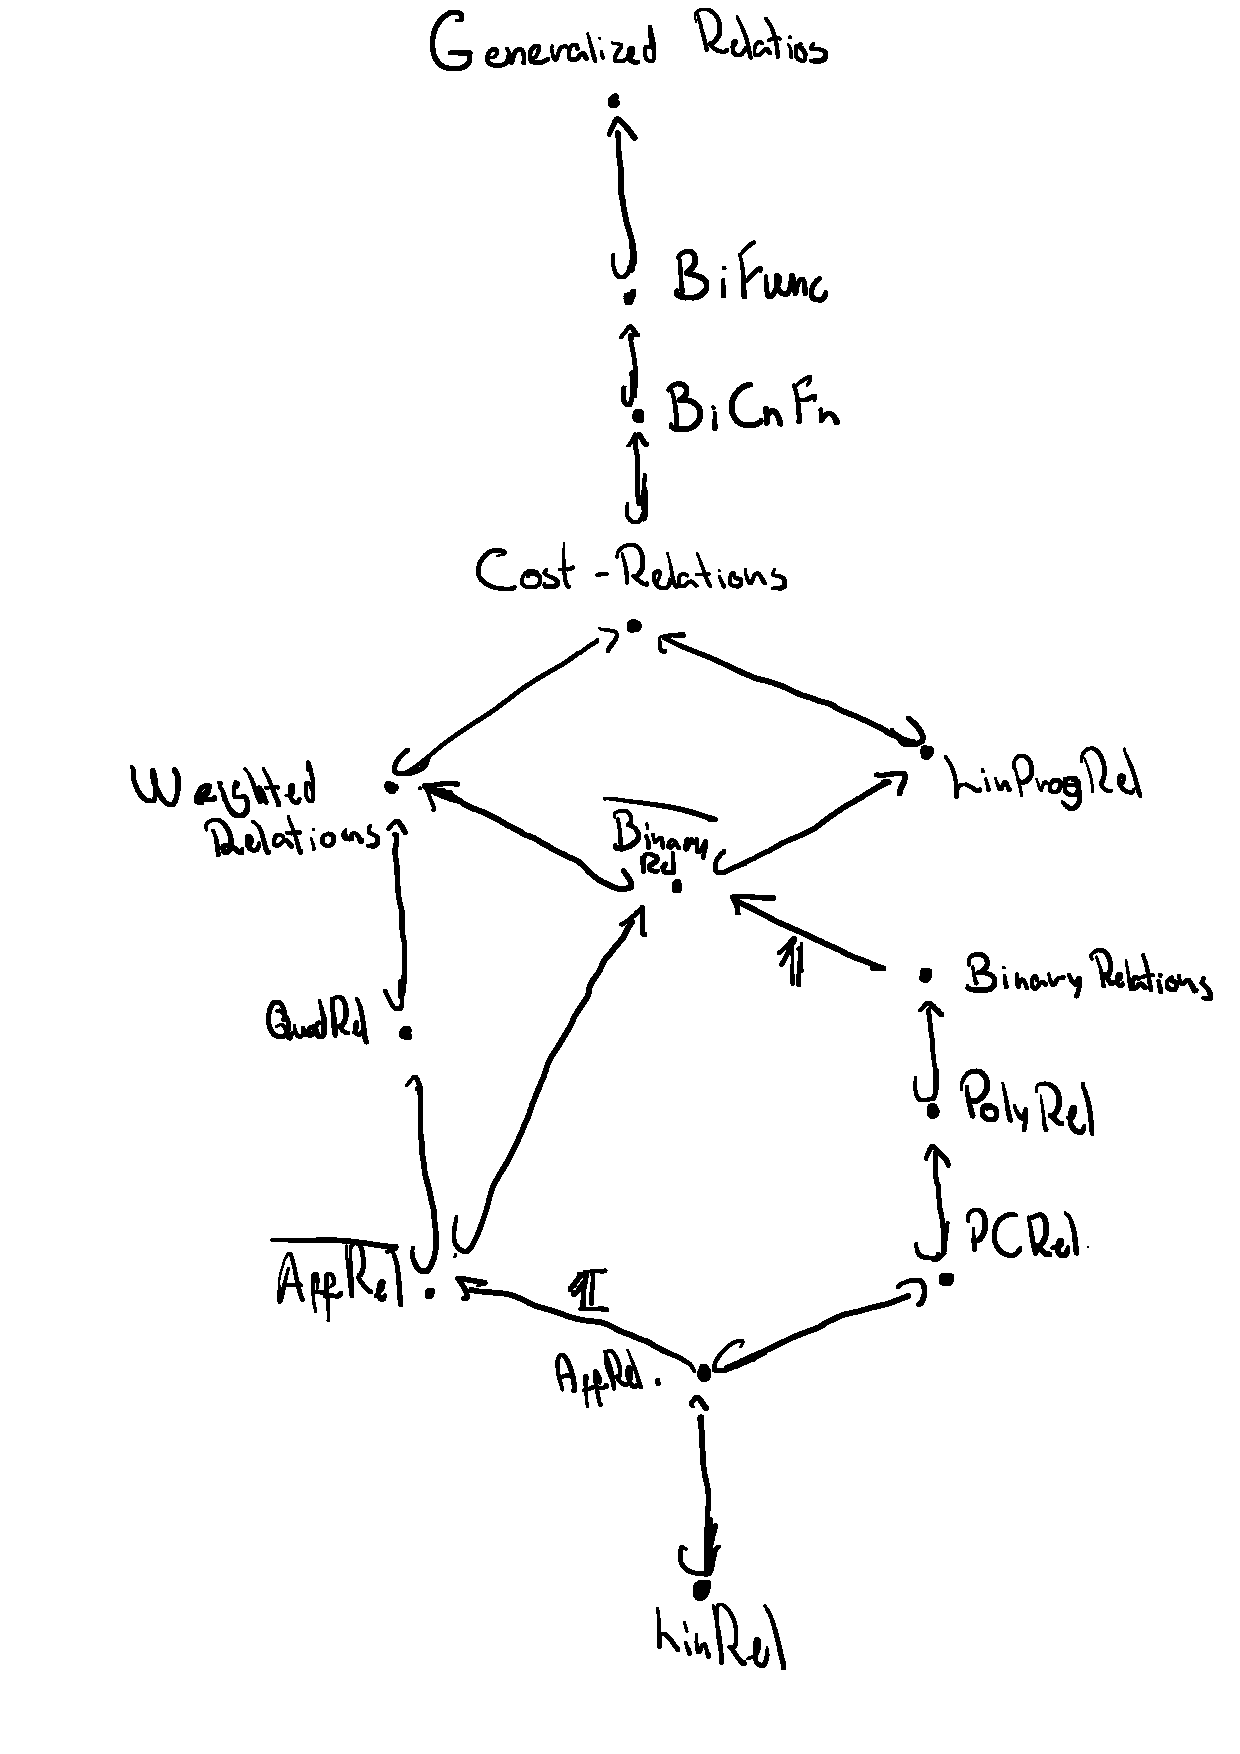
\includegraphics[width=1.0\linewidth]{images/Overview.pdf}
    \caption{The hierarchy of relational categories developed in this
    thesis. Each inclusion preserves the monoidal and compositional
    structure of the layer below.}
    \label{fig:overview}
\end{figure}


\printbibliography
\end{document}
